% Курсова робота з ОК «Моделювання систем. Курсова робота», варіант B14.
% Структура — за вказівками лектора та розд. 4 навчального посібника (Стеценко та ін., 2024).
\documentclass[coursework]{kpi-thesis}
\usepackage{kpi-titles}
% Формули -- гарнітурою, сумісною з Times New Roman основного тексту: клас
% лишає Computer Modern. XeLaTeX -> unicode-math; \mathrm, \text -- шрифт тексту (Times New Roman).
\usepackage{unicode-math}
\setmathfont{STIXTwoMath-Regular.otf}
% Міжрядковий інтервал 1,5 (розд. 4.5 посібника) — як у Word: 1,5 × 1,15 × 14 пт ≈ 24,15 пт.
% \onehalfspacing класу для 14 пт дає множник 1,25 від бази 17 пт = 21,25 пт (≈ «1,3» у Word).
\setstretch{1.42}
% Схеми процесу (розділ 1) — TikZ, щоб текст на рисунках мав шрифт роботи
\usepackage{tikz}
\usetikzlibrary{positioning,arrows.meta,shapes.geometric,shapes.multipart,fit,calc,backgrounds}
% Відмінності від методички диплома — за вказівками лектора до курсової (розд. «Оформлення
% пояснювальної записки») та розд. 4.5 / Додатками А–Б навчального посібника:
\kpisetup{
  left-margin    = 20mm,   % «поля ліве, праве, зверху та знизу – 20 мм»
  hyphenation    = false,  % «Переноси слів не потрібно використовувати» (розд. 4.5 посібника)
  enumerate      = arabic, % пункти завдання «1)», «2)» (Додаток Б посібника)
  appendix-title = inline, % «Додаток А. Лістинг коду …» (розд. 4.5 посібника)
  algorithms,              % псевдокод алгоритму імітації (розділ 3)
}
% Заголовок додатка у ЗМІСТІ -- так само, як у тексті: «Додаток А. Лістинг …».
% Клас пише в зміст «Додаток А Лістинг …» без крапки; визначення \appendix класу (appendix-title =
% inline) повторено тут з крапкою в \addcontentsline, копію класу не змінюємо.
\makeatletter
\RenewDocumentCommand\appendix{o m}{%
  \clearpage
  \refstepcounter{section}%
  \global\advance\c@kpi@appendices\@ne
  \IfValueT{#1}{\label{#1}}%
  {\centering Додаток \thesection.\ \textbf{#2}\par}%
  \addcontentsline{toc}{section}{Додаток \thesection.\ #2}%
  \vspace{\baselineskip}%
}
\makeatother
% Підпис таблиці: з абзацного відступу 1,25 см (типове значення класу, ДСТУ 3008:2015 п. 7.6.8)
% і по ширині рядка (вказівки лектора: «згори таблиці з вирівнюванням по ширині»).
\captionsetup*[table]{justification=justified}
% Підписи рисунків і таблиць -- з тим самим інтервалом 1,5, що й текст (\setstretch вище):
% longtable і плаваючі обʼєкти інакше скидають міжрядковий інтервал до одинарного.
\captionsetup{font+={stretch=1.42}}
% Клас задає \LTcapwidth=\textwidth до left-margin=20mm (текст ще 160 мм), тож підписи longtable
% (kpitable) центруються у вужчому блоці й зсуваються на 5 мм. Перевиставити за поточною шириною.
\AtBeginDocument{\setlength{\LTcapwidth}{\textwidth}}
\kpiset{
  title         = {Імітаційна модель інформаційної системи обробки завдань трьох типів з пріоритетним
                   упорядкуванням черги на основі формального опису стохастичною мережею Петрі},
  discipline    = {Моделювання систем. Курсова робота},
  group         = {ІП-33},
  course        = {IV},
  gender        = {m},
  student       = {Хребтань Максим Віталійович},
  gradebook     = {24},
  advisor       = {Коринецький Дмитро Сергійович},
  year          = {2026},
}
% Поле титулу за Додатком А посібника, якого немає в kpiset
\newcommand\cwAdvisorShort{Дмитро КОРИНЕЦЬКИЙ}

% Число з іменником у потрібній формі для анотації: \cwStat{tables}{таблицю}{таблиці}{таблиць} ->
% «24 таблиці». Значення -- з build/main.kpistats (\kpiloadstats в анотації), до першої збірки «??».
\ExplSyntaxOn
\NewDocumentCommand\cwStat{mmmm}{
  \cs_if_exist:cTF { kpi@stat@main@#1 }
    {
      \int_set:Nn \l_tmpa_int { \use:c { kpi@stat@main@#1 } }
      \int_use:N \l_tmpa_int \nobreakspace
      \int_set:Nn \l_tmpb_int { \int_mod:nn { \l_tmpa_int } { 100 } }
      \bool_if:nTF { \int_compare_p:n { 11 <= \l_tmpb_int <= 14 } } {#4}
        {
          \int_case:nnF { \int_mod:nn { \l_tmpa_int } { 10 } }
            { {1} {#2} {2} {#3} {3} {#3} {4} {#3} }
            {#4}
        }
    }
    { \textbf{??}~#4 }
}
\ExplSyntaxOff

% Ключові слова псевдокоду (algpseudocode) українською
% Репозиторій з повним кодом програми й експериментів (Р3, додатки А і В)
\newcommand\repourl{\url{https://github.com/mkhrebtan/b14-petri-simulation}}
\algrenewcommand\algorithmicrequire{\textbf{Вхідні дані:}}
\algrenewcommand\algorithmicif{\textbf{якщо}}
\algrenewcommand\algorithmicthen{\textbf{то}}
\algrenewcommand\algorithmicelse{\textbf{інакше}}
\algrenewcommand\algorithmicfor{\textbf{для}}
\algrenewcommand\algorithmicforall{\textbf{для всіх}}
\algrenewcommand\algorithmicwhile{\textbf{поки}}
\algrenewcommand\algorithmicdo{\textbf{виконувати}}
\algrenewcommand\algorithmicloop{\textbf{повторювати}}
\algrenewcommand\algorithmicprocedure{\textbf{процедура}}
% Фрагменти коду в основному тексті (Р3--Р5) -- 10 пт, без додаткових
% вертикальних відступів навколо фрагмента (інакше Р3 виходить на 15-ту сторінку трьома рядками);
% спільний відступ рядків прибирає gobble у кожному \codeinput. Лістинги додатків -- 8 пт класу
% (\fvset перед \appendices), інакше додатки перевищать 35 с.
\fvset{fontsize=\setstretch{1}\fontsize{10}{11}\selectfont,
  listparameters={\setlength\topsep{0pt}\setlength\partopsep{0pt}}}
% Лістинг одного файлу програми моделі (sim/src/main/java/ua/kpi/km/b14/<шлях>)
\newcommand\javafile[1]{\par\medskip\Needspace{4\baselineskip}\noindent\textbf{Файл \texttt{#1}}\par
  \codeinput{../sim/src/main/java/ua/kpi/km/b14/#1}}
% Фрагмент скрипта статистичної обробки: \pyfrag{назва}{перший рядок}{останній рядок}
\newcommand\pyfrag[3]{\par\medskip\Needspace{4\baselineskip}\noindent\textbf{#1 (рядки #2--#3)}\par
  \codeinput[firstline=#2, lastline=#3]{../experiments/analysis.py}}

\begin{document}
% Титульна сторінка за Додатком А навчального посібника (Стеценко, Дифучина, Дифучин, 2024).
\makeatletter
\begingroup
\newgeometry{left=20mm,right=20mm,top=20mm,bottom=20mm}%
\thispagestyle{empty}%
% Шапка й блок теми — інтервал 1,5 (як у зразку), блок підписів — одинарний.
\begin{center}

\includegraphics[width=105mm]{media/kpi-building.png}

\vspace{0.4cm}
МІНІСТЕРСТВО ОСВІТИ І НАУКИ УКРАЇНИ

НАЦІОНАЛЬНИЙ ТЕХНІЧНИЙ УНІВЕРСИТЕТ УКРАЇНИ

«КИЇВСЬКИЙ ПОЛІТЕХНІЧНИЙ ІНСТИТУТ імені ІГОРЯ СІКОРСЬКОГО»

КАФЕДРА ІНФОРМАТИКИ ТА ПРОГРАМНОЇ ІНЖЕНЕРІЇ

\vspace{1.6cm}
Курсова робота з освітнього компоненту

«\kpi@g{discipline}»

\vspace{0.3cm}
Тема: \textbf{\kpi@g{title}}
\end{center}

\vspace{1.2cm}
\setstretch{1.0}%
\noindent
\begin{minipage}[t]{0.47\textwidth}
\raggedright
\textbf{Керівник:}

\kpi@g{advisor}

\vspace{0.6cm}
«Допущено до захисту»

\sigline{5cm}

\vspace{0.3cm}
«\sigline{0.8cm}» \sigline{3cm} 20\sigline{0.6cm} р.

\vspace{0.6cm}
Захищено з оцінкою

\sigline{5cm}

\vspace{0.6cm}
Члени комісії:

\vspace{0.3cm}
\sigline{5cm}

\vspace{0.3cm}
\sigline{5cm}
\end{minipage}%
\hfill
\begin{minipage}[t]{0.47\textwidth}
\raggedright
\textbf{Виконавець:}

\kpi@g{student}

студент групи \kpi@g{group}

залікова книжка № \kpi@gradebook

\sigline{5cm}

\vspace{0.3cm}
«\sigline{0.8cm}» \sigline{3cm} 20\sigline{0.6cm} р.

\vspace{3.15cm}
\vspace{0.3cm}
Інна СТЕЦЕНКО

\vspace{0.6cm}
\cwAdvisorShort
\end{minipage}

\vfill
\begin{center}
\textbf{Київ -- \kpi@g{year}}
\end{center}
\restoregeometry
\endgroup
\clearpage
\makeatother

\mainmatter
% Порядок за вказівками лектора (таблиця «Зміст розділів»): анотація → вступ → завдання;
% зміст — після анотації (розд. 4.1 посібника). Посібник ставить завдання після титулу,
% але в разі розбіжності пріоритет за вимогами лектора.
% Анотація — за Додатком В навчального посібника (не менше 650 символів).
% Кількості сторінок, рисунків, таблиць, джерел і додатків — з build/main.kpistats попередньої
% збірки (клас kpi-thesis записує їх наприкінці документа; latexmk перезбирає, доки не зійдеться).
\kpiloadstats{main}{build/main.kpistats}
\structural{АНОТАЦІЯ}

Хребтань Максим Віталійович. Курсова робота на тему «\kpiTitle».

Текстова частина курсової роботи складається із вступу, пʼяти розділів, висновків, списку
використаних джерел з \cwStat{sources}{найменування}{найменувань}{найменувань} та
\cwStat{appendices}{додатка}{додатків}{додатків}, які викладено на
\cwStat{pages}{сторінці}{сторінках}{сторінках}. В тексті роботи оформлено
\cwStat{figures}{рисунок}{рисунки}{рисунків}, \cwStat{tables}{таблицю}{таблиці}{таблиць}.

У роботі поставлено завдання дослідити, як пʼять стратегій пріоритетного упорядкування черги за
різних інтенсивностей надходження впливають на середній час перебування завдання в системі,
середню кількість завдань у черзі та середній час очікування в інформаційній системі, що обробляє
завдання трьох типів зі спільною оперативною памʼяттю: завдання A і~B можуть виконуватися
одночасно, а завдання~C монополізує систему.

Імітаційна модель розроблена на основі формального опису системи стохастичною мережею Петрі, у
якій обмеження на одночасне виконання задано кратністю дуг, а стратегії -- пріоритетами та
ймовірностями запуску переходів. Алгоритм імітації реалізовано мовою Java на основі ядра
бібліотеки PetriObjModelPaint, розширеного класами-нащадками; коректність моделі підтверджено
верифікацією. Статистичну обробку виконано мовою Python.

Проведено дослідження: визначено перехідний період, час моделювання й кількість прогонів,
виконано повний факторний експеримент «стратегія $\times$ інтенсивність» (2100~прогонів),
дисперсійний і регресійний аналіз.

Результати моделювання свідчать, що за інтенсивностей з умови задачі система перевантажена за
будь-якої стратегії, а в області стійкості найменші значення всіх трьох показників дають
стратегії з найнижчим пріоритетом завдань~C -- середній час перебування в них до 2,3~раза менший,
ніж у стратегіях з пріоритетом~C, коштом довшого очікування завдань~C.

Зроблено висновки щодо вибору стратегії упорядкування і запропоновано збільшити памʼять системи
до трьох умовних одиниць; пробний запуск показав, що система стає стійкою за інтенсивностей з
умови задачі, а за зменшеного потоку середній час перебування скорочується на 70--86~\%, тож для
потоку, близького до заданого, ця зміна ресурсу доцільна.

\noindent Ключові слова: імітаційна модель, алгоритм імітації, стохастична мережа Петрі,
стратегія упорядкування черги, пріоритетне обслуговування, факторний експеримент, дисперсійний
аналіз, Java.

\tableofcontents

\structural{ВСТУП}

Інформаційні системи, що обробляють потік завдань різних типів на спільних обчислювальних
ресурсах, мають вирішувати, у якому порядку обслуговувати завдання, що очікують. Від стратегії
упорядкування черги залежать час відповіді системи, кількість завдань, що накопичуються, і
розподіл очікування між типами завдань. Аналітичні методи теорії масового обслуговування дають
точні результати лише для простих систем, а в системі, де завдання займають різну частку
ресурсу, одне з них монополізує систему, а пріоритет вимагає резервувати ресурс, точний
аналітичний розвʼязок отримати складно. Експерименти з реальною системою дорогі й небезпечні
для її користувачів. Тому актуальним методом дослідження є імітаційне моделювання, яке дає
змогу відтворити функціонування системи з урахуванням усіх правил і оцінити вплив стратегій
до їх впровадження.

Тема курсової роботи -- «\kpiTitle». Обʼєкт дослідження -- інформаційна система, яка обробляє
завдання трьох типів (A, B, C), що конкурують за оперативну памʼять: завдання A і~B можуть
виконуватися одночасно, а завдання~C монополізує систему. Предмет дослідження -- вплив стратегії
упорядкування черги на показники обслуговування.

Мета роботи -- визначити вплив пʼяти стратегій упорядкування черги за різних інтенсивностей
надходження завдань на середній час перебування завдання в системі, середню кількість завдань у
черзі та середній час очікування в черзі, а також запропонувати шляхи поліпшення
функціонування системи.

Для досягнення мети розроблено концептуальну модель системи, її формалізовано стохастичною
мережею Петрі~\cite{stetsenko-kursova, stetsenko-modeling}, у якій обмеження на одночасне
виконання завдань задано кратністю дуг, а стратегії упорядкування -- пріоритетами та
ймовірностями запуску переходів. Алгоритм імітації мережі Петрі реалізовано мовою
Java~\cite{java-jls} на основі ядра бібліотеки PetriObjModelPaint~\cite{petriobjmodelpaint},
розширеного засобами обʼєктно-орієнтованого програмування; збірку виконує Apache
Maven~\cite{maven}, тести -- JUnit~5~\cite{junit}. Коректність моделі перевірено верифікацією:
контролем інваріантів мережі, аналізом реакції відгуків на зміну вхідних змінних і порівнянням з
аналітичними результатами для систем M/M/1 і M/M/2~\cite{kleinrock}. Експериментальне дослідження виконано за повним факторним планом
«стратегія $\times$ інтенсивність надходження» з визначенням перехідного періоду, часу
моделювання й кількості прогонів; результати оброблено дисперсійним і регресійним
аналізом мовою Python з бібліотекою SciPy~\cite{scipy}. Пропозицію щодо поліпшення системи оцінено пробним запуском
моделі.

% Завдання до курсової роботи — за Додатком Б навчального посібника.
\structural{ЗАВДАННЯ}

Виконати дослідження для такої системи.

На обробку до інформаційної системи приймаються три типи завдань A, B і C. Виходячи з наявності
оперативної памʼяті обчислювальної системи, завдання типів A і B можуть виконуватися одночасно. Тобто
завдання типу A можуть виконуватися паралельно із завданням свого класу або із завданням типу B.
Аналогічно, завдання типу B можуть виконуватися паралельно із завданням свого класу або із завданням
типу A. Завдання типу C монополізують інформаційну систему. Завдання надходять у середньому з
інтенсивністю 0,2~завдання/хв, 0,07~завдання/хв, 0,06~завдання/хв для класів A, B та C відповідно.
Завдання виконуються протягом часу, що є випадковою величиною, розподіленою за експоненціальним законом
з інтенсивністю 0,25~завдання/хв, 0,2~завдання/хв, 0,1~завдання/хв для класів A, B та C відповідно.

Упорядкування в черзі на обслуговування визначається комбінацією пріоритетів завдань. Можливі такі
комбінації:
\begin{itemize}
\item A -- вищий, B -- середній, C -- низький;
\item B -- вищий, A -- середній, C -- низький;
\item C -- вищий, B -- середній, A -- низький;
\item C -- вищий, A -- середній, B -- низький;
\item C -- вищий, A і B -- низький.
\end{itemize}

Метою моделювання є визначення впливу різних стратегій упорядкування в черзі при різних значеннях
інтенсивності надходження на такі параметри інформаційної системи: середній час обслуговування завдання
в системі; середня кількість завдань, що очікують обслуговування; середній час очікування в чергах.

Для вищезазначеної системи:
\begin{enumerate}
\item розробити опис концептуальної моделі системи;
\item виконати формалізацію опису обʼєкта моделювання в термінах стохастичної мережі Петрі;
\item розробити алгоритм імітації моделі дискретно-подійної системи у відповідності до побудованого
  формального опису;
\item для доведення коректності побудованого алгоритму виконати верифікацію алгоритму імітації;
\item визначити статистичні оцінки заданих характеристик моделі, що є метою моделювання;
\item провести експериментальне дослідження моделі;
\item інтерпретувати результати моделювання та сформулювати пропозиції щодо поліпшення функціонування
  системи;
\item зробити висновки щодо складності розробки моделі та алгоритму імітації на основі використаного
  формалізму, отриманих результатів моделювання та їх корисності.
\end{enumerate}

\section{Концептуальна модель системи}

Обʼєкт моделювання -- інформаційна система, що виконує завдання типів A, B і~C на одній
обчислювальній системі зі спільною оперативною памʼяттю; завдання, які не можуть стартувати одразу,
чекають у черзі, порядок вибору з якої задає одна з пʼяти стратегій. Часові величини вимірюються у хвилинах (умовна одиниця модельного часу -- 1~хв),
інтенсивності -- у завданнях за хвилину.

\subsection{Склад системи та звʼязки між елементами}

Структура системи (рисунок~\ref{fig:structure}) містить такі елементи:
\begin{enumerate}
  \item три незалежні джерела завдань типів A, B і~C з інтенсивностями $\lambda_A$, $\lambda_B$, $\lambda_C$;
  \item черга, упорядкована за пріоритетами типів: три підчерги (по одній на тип) з FIFO
        всередині, довжина не обмежена, завдання не втрачаються;
  \item диспетчер, що обирає наступне завдання для запуску за чинною стратегією~$s$;
  \item обчислювальна підсистема з оперативною памʼяттю -- єдиним спільним обмеженим ресурсом.
\end{enumerate}

Умова задає лише середні інтенсивності, тож прийнято припущення про пуассонівські потоки з
інтервалами $\exp(1/\lambda_i)$ -- від багатьох незалежних користувачів; час виконання за умовою
експоненційний з~$\mu_i$.

Обмеження на одночасне виконання умова формулює так: завдання типу~A «можуть виконуватися
паралельно із завданням свого класу або із завданням типу~B», аналогічно для~B, а завдання
типу~C монополізують систему. Граничну кількість одночасних завдань прямо не вказано, тому
прийнято припущення: одночасно виконуються не більше двох завдань (пари AA, AB, BB), бо
в умові вжито однину -- «із завданням», тобто напарник щонайбільше один. Його відтворено обсягом
памʼяті $M=2$~умовні одиниці: A і~B займають по $v_A=v_B=1$~од., C -- $v_C=2$~од., тобто всю
памʼять (монополізація). Допустимі стани: порожня, A, B, AA, AB, BB, C. Наслідки іншого
тлумачення оцінює зміна~$M$ (розділи~3 і~5).

\begin{figure}
  \centering
  % Рисунок 1.1 — структура інформаційної системи (концептуальна модель)
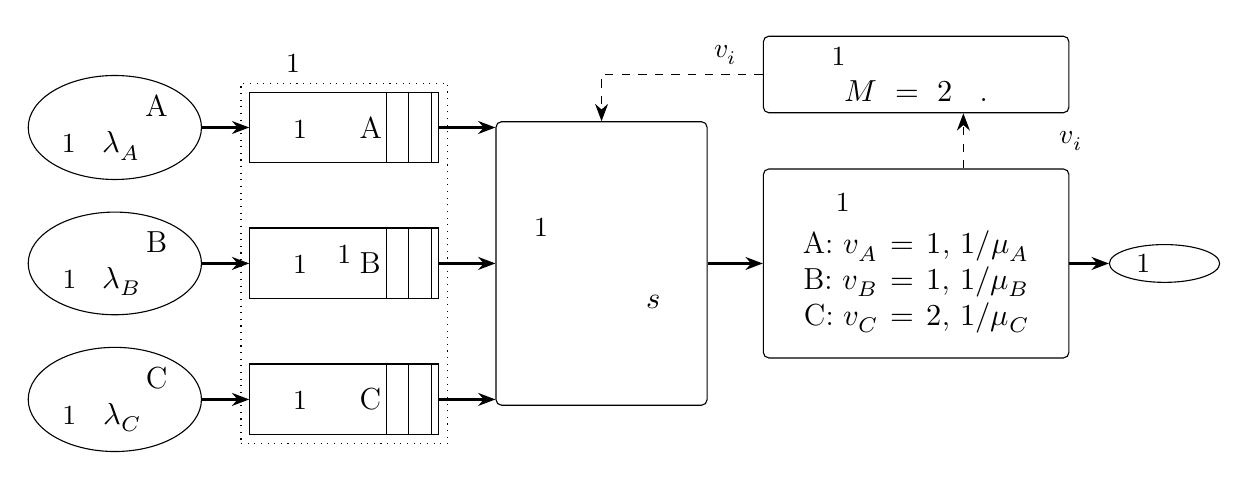
\begin{tikzpicture}[
    font=\setstretch{1}\fontsize{11}{13}\selectfont, >={Stealth[length=2.2mm]}, node distance=4mm and 6mm,
    src/.style={draw, ellipse, align=center, inner sep=1.5pt, minimum width=22mm},
    queue/.style={draw, rectangle, minimum width=24mm, minimum height=9mm, align=left, text width=13mm},
    blk/.style={draw, rectangle, rounded corners=2pt, align=center, inner sep=4pt},
    flow/.style={->, thick},
    res/.style={->, dashed},
  ]
  % Джерела
  \node[src] (sA) {Джерело A\\$\lambda_A$};
  \node[src, below=of sA] (sB) {Джерело B\\$\lambda_B$};
  \node[src, below=of sB] (sC) {Джерело C\\$\lambda_C$};
  % Черги
  \node[queue, right=of sA] (qA) {Черга A};
  \node[queue, right=of sB] (qB) {Черга B};
  \node[queue, right=of sC] (qC) {Черга C};
  \foreach \q in {qA,qB,qC}{
    \foreach \x in {0.72,0.84,0.96}{
      \draw ($(\q.north west)!\x!(\q.north east)$) -- ($(\q.south west)!\x!(\q.south east)$);
    }
  }
  \node[draw, dotted, inner sep=3pt, fit=(qA)(qC), label={[align=center]above:Упорядкована\\черга}] (Q) {};
  % Диспетчер
  \node[blk, right=6mm of Q, minimum height=36mm, text width=24mm] (disp)
    {Вибір завдання за~стратегією пріоритетів~$s$};
  % Обробка
  \node[blk, right=7mm of disp, text width=36mm, minimum height=24mm] (cpu)
    {Виконання завдань\\[2pt]
     A: $v_A=1$, $1/\mu_A$\\
     B: $v_B=1$, $1/\mu_B$\\
     C: $v_C=2$, $1/\mu_C$};
  \node[blk, above=7mm of cpu, text width=36mm] (mem) {Оперативна памʼять\\$M=2$ од.};
  \node[src, minimum width=14mm, right=5mm of cpu] (out) {Вихід};
  % Зв'язки
  \draw[flow] (sA) -- (qA);
  \draw[flow] (sB) -- (qB);
  \draw[flow] (sC) -- (qC);
  \draw[flow] (qA.east) -- (qA.east -| disp.west);
  \draw[flow] (qB.east) -- (qB.east -| disp.west);
  \draw[flow] (qC.east) -- (qC.east -| disp.west);
  \draw[flow] (disp.east |- cpu) -- (cpu.west);
  \draw[flow] (cpu) -- (out);
  \draw[res] (mem.west) -| node[pos=0.25, above, font=\fontsize{10}{12}\selectfont] {захоплення $v_i$} (disp.north);
  \draw[res] ([xshift=6mm]cpu.north) -- node[right, font=\fontsize{10}{12}\selectfont] {звільнення $v_i$} ([xshift=6mm]mem.south);
\end{tikzpicture}

  \caption{Структура інформаційної системи обробки завдань}
  \label{fig:structure}
\end{figure}

Стратегії упорядкування з умови наведено в таблиці~\ref{tab:strategies}.

\begin{kpitable}{|L{3.4cm}|c|c|c|c|c|}{Стратегії упорядкування черги\label{tab:strategies}}
  {\textbf{Стратегія $s$} & \textbf{1} & \textbf{2} & \textbf{3} & \textbf{4} & \textbf{5}}
  Упорядкування & A $>$ B $>$ C & B $>$ A $>$ C & C $>$ B $>$ A & C $>$ A $>$ B & C $>$ (A $=$ B) \\ \hline
\end{kpitable}

\subsection{Опис процесу функціонування системи}\label{sec:process}

Завдання типу~$i$ стає в кінець своєї підчерги, починає виконуватися, щойно справджуються умови
старту (рисунок~\ref{fig:process}), а після виконання звільняє памʼять і виходить із системи.
Умови перевіряють після кожного надходження й звільнення памʼяті; за двох вільних одиниць можуть
одночасно стартувати два завдання A/B.

Умова визначає упорядкування саме в черзі, тож черга -- єдина впорядкована послідовність, яку
обслуговують з початку. Звідси правила:
\begin{itemize}
  \item резервування для завдань вищого пріоритету: завдання нижчого пріоритету не обходить
        завдання вищого пріоритету, що очікує, навіть за вільної памʼяті (інакше в стратегіях
        3--5 завдання~C майже не отримувало б усю памʼять); у стратегіях 1--2 C стартує лише за
        порожніх підчерг A і~B;
  \item обслуговування без переривання: пріоритет діє лише під час вибору наступного завдання;
  \item рівні пріоритети (стратегія~5): якщо на одну вільну одиницю памʼяті претендують
        завдання~A і~B, запускається одне з них з імовірностями $0{,}5$.
\end{itemize}

\begin{figure}
  \centering
  % Рисунок 1.2 — процес проходження одного завдання типу i через систему
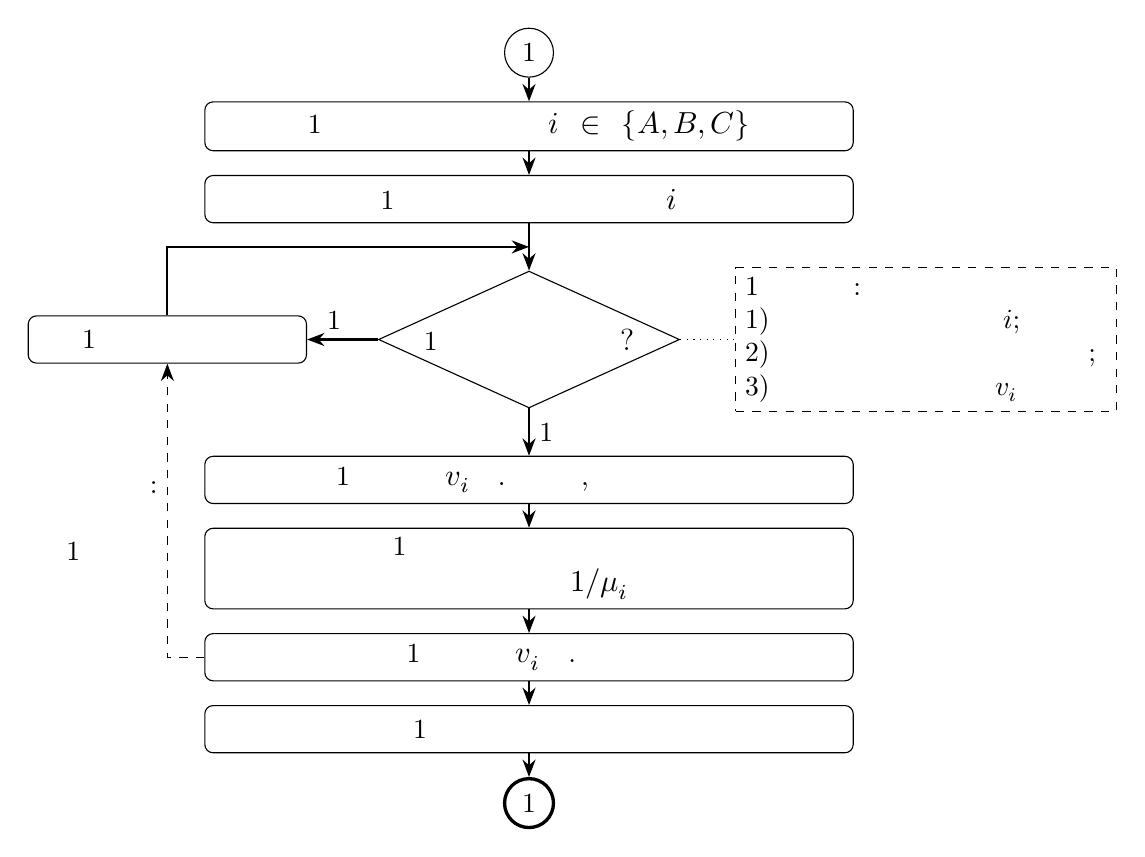
\begin{tikzpicture}[
    font=\setstretch{1}\fontsize{11}{13}\selectfont, >={Stealth[length=2.2mm]}, node distance=3mm,
    ev/.style={draw, circle, minimum size=6mm},
    act/.style={draw, rectangle, rounded corners=3pt, align=center, text width=80mm, minimum height=6mm},
    dec/.style={draw, diamond, aspect=2.2, align=center, text width=30mm, inner sep=1pt},
    note/.style={draw, dashed, rectangle, align=left, text width=46mm, font=\setstretch{1}\fontsize{10}{12}\selectfont},
    flow/.style={->, thick},
  ]
  \node[ev] (start) {};
  \node[act, below=of start] (arr) {Надходження завдання типу $i\in\{A,B,C\}$};
  \node[act, below=of arr] (enq) {Постановка в кінець черги типу $i$};
  \node[dec, below=6mm of enq] (cond) {Умови старту виконано?};
  \node[act, below=6mm of cond] (take) {Захоплення $v_i$ од. памʼяті, вихід із черги};
  \node[act, below=of take] (serv) {Виконання протягом випадкового\\часу з~середнім $1/\mu_i$};
  \node[act, below=of serv] (rel) {Звільнення $v_i$ од. памʼяті};
  \node[act, below=of rel] (dep) {Вихід завдання із системи};
  \node[ev, very thick, below=of dep] (end) {};
  \node[act, text width=33mm, left=9mm of cond] (wait) {Очікування в черзі};
  \node[note, right=7mm of cond] (cn) {Умови старту:\\
    1) завдання перше в черзі типу $i$;\\
    2) у черзі немає завдань вищого пріоритету;\\
    3) вільна памʼять не менша за $v_i$};

  \draw[flow] (start) -- (arr);
  \draw[flow] (arr) -- (enq);
  \draw[flow] (enq) -- (cond);
  \draw[flow] (cond) -- node[right] {так} (take);
  \draw[flow] (cond.west) -- node[above] {ні} (wait.east);
  \draw[flow] (wait.north) |- ($(enq.south)!0.5!(cond.north)$);
  \draw[flow] (take) -- (serv);
  \draw[flow] (serv) -- (rel);
  \draw[flow] (rel) -- (dep);
  \draw[flow] (dep) -- (end);
  \draw[dotted] (cond.east) -- (cn.west);
  \draw[->, dashed] (rel.west) -| node[pos=0.75, left, align=right, font=\setstretch{1}\fontsize{10}{12}\selectfont]
    {звільнення\\памʼяті:\\повторна\\перевірка} (wait.south);
\end{tikzpicture}

  \caption{Процес проходження завдання типу~$i$ через систему}
  \label{fig:process}
\end{figure}

Спрощення: час виконання не залежить від паралельного виконання іншого завдання, затримки
диспетчеризації нехтовні.

За інтенсивностей з умови задачі система перевантажена: частка памʼяті, потрібна для
обслуговування всього потоку, становить
\begin{equation}\label{eq:rho}
  \rho = \frac{1}{M}\sum_{i\in\{A,B,C\}} \frac{\lambda_i v_i}{\mu_i}
       = \frac{1}{2}\left(\frac{0{,}2}{0{,}25} + \frac{0{,}07}{0{,}2}
          + \frac{0{,}06\cdot 2}{0{,}1}\right) = 1{,}175 > 1,
\end{equation}
тож черги зростають необмежено за будь-якої стратегії. Тому інтенсивності всіх типів
варіюються спільним коефіцієнтом~$\gamma$: $\lambda_i = \gamma\lambda_i^0$, де $\lambda_i^0$ --
значення з умови. Необхідна умова стійкості $\gamma\cdot 1{,}175<1$ дає $\gamma<0{,}85$; через
простоювання памʼяті під час резервування фактична межа нижча й залежить від стратегії (розділ~4).

\subsection{Вхідні змінні та параметри моделі}

Вхідні змінні наведено в таблиці~\ref{tab:inputs}, параметри -- у таблиці~\ref{tab:params};
$\exp(a)$ -- експоненційна випадкова величина із середнім~$a$~\cite{stetsenko-kursova}.

\begin{kpitable}{|L{4.6cm}|c|L{2.4cm}|L{2.7cm}|L{3.1cm}|}{Вхідні змінні моделі\label{tab:inputs}}
  {\textbf{Змінна} & \textbf{Позначення} & \textbf{Початкове значення} & \textbf{Діапазон} & \textbf{Закон розподілу}}
  Стратегія упорядкування черги & $s$ & 1 & $\{1,\dots,5\}$, табл.~\ref{tab:strategies} & детермінована \\ \hline
  Коефіцієнт інтенсивності надходження & $\gamma$ & 1 & $[0{,}4;\ 1{,}0]$ & детермінована \\ \hline
  Інтенсивності надходження A, B, C, завд./хв & $\lambda_A, \lambda_B, \lambda_C$ &
    $0{,}2$\newline $0{,}07$\newline $0{,}06$ &
    $[0{,}08;\ 0{,}2]$\newline $[0{,}028;\ 0{,}07]$\newline $[0{,}024;\ 0{,}06]$ &
    пуассонівські, інтервали $\exp(1/\lambda_i)$~хв \\ \hline
\end{kpitable}

Незалежні фактори -- лише $s$ і~$\gamma$, інтенсивності $\lambda_i=\gamma\lambda_i^0$ похідні;
окремо їх змінюють лише у верифікації (розділ~3) і пробній серії розділу~4.

\begin{kpitable}{|L{6.2cm}|c|L{7.2cm}|}{Параметри моделі\label{tab:params}}
  {\textbf{Параметр} & \textbf{Позначення} & \textbf{Значення}}
  Інтенсивності виконання A, B, C & $\mu_A, \mu_B, \mu_C$ &
    $0{,}25$; $0{,}2$; $0{,}1$~завд./хв, час $\exp(4)$, $\exp(5)$, $\exp(10)$~хв \\ \hline
  Обсяг оперативної памʼяті & $M$ & 2~умовні одиниці \\ \hline
  Потреба A, B, C у памʼяті & $v_A, v_B, v_C$ & 1; 1; 2~умовні одиниці \\ \hline
  Ємність черги & -- & необмежена \\ \hline
  Ймовірності вибору A і~B за рівних пріоритетів & -- & $0{,}5$; $0{,}5$ (лише стратегія~5) \\ \hline
  Час моделювання, тривалість перехідного періоду & $T_{\text{мод}}$, $T_{\text{п}}$ &
    обґрунтовуються в розділі~4 \\ \hline
\end{kpitable}

\subsection{Вихідні змінні моделі}

Вихідні змінні (таблиця~\ref{tab:outputs}; формули -- у розділі~2) визначають для кожного типу
і загалом (середні за всіма завданнями), бо підвищення пріоритету одного типу скорочує його
очікування за рахунок інших; «середній час обслуговування в системі» тлумачимо як час перебування.

\begin{kpitable}{|L{4.3cm}|c|c|L{6.9cm}|}{Вихідні змінні моделі\label{tab:outputs}}
  {\textbf{Змінна} & \textbf{Позначення} & \textbf{\makecell{Одиниці\\виміру}} & \textbf{Що спостерігається під час імітації}}
  Середній час перебування в системі & $W_i$, $W$ & хв &
    кількість завдань типу~$i$ у системі (середня за часом), надходжень \\ \hline
  Середня кількість завдань, що очікують обслуговування & $L_{q,i}$, $L_q$ & завд. &
    середня за часом довжина підчерги типу~$i$ \\ \hline
  Середній час очікування в черзі & $W_{q,i}$, $W_q$ & хв &
    довжина підчерги (середня за часом), кількість надходжень \\ \hline
  Коефіцієнт використання памʼяті (допоміжна) & $U$ & -- &
    середня за часом кількість зайнятих одиниць памʼяті${}/M$ \\ \hline
\end{kpitable}


\subsection{Висновки до розділу}

Умову конкретизовано припущеннями (пуассонівські потоки, не більше двох одночасних завдань,
резервування, без переривання), через перевантаження ($\rho=1{,}175$) інтенсивності варіюють
коефіцієнтом~$\gamma$; вхідні ($s$, $\gamma$) і вихідні ($W$, $L_q$, $W_q$) змінні відповідають меті.

\section{Формалізована модель системи}

Для формалізації обрано стохастичну мережу Петрі з позначеннями за таблицею позначень~3.2
посібника~\cite{stetsenko-kursova}: позиція (кількість маркерів~$m$), дуга (кратність~$k$), перехід
(затримка~$d$, пріоритет~$r$, ймовірність запуску~$b$). Часткове захоплення спільної памʼяті
задається кратністю дуг, конкуренція подій за ресурс -- спільною вхідною позицією, а стратегія
упорядкування -- пріоритетами та ймовірностями запуску. Мережу побудовано й перевірено в
редакторі й симуляторі PetriObjModelPaint~\cite{petriobjmodelpaint}.

\subsection{Стохастична мережа Петрі моделі}

Подіям концептуальної моделі (рисунок~\ref{fig:process}) відповідають переходи: надходження
й виконання завдання типу~$i$ і резервування памʼяті для завдання~C (рисунок~\ref{fig:petri};
штрихова стрілка -- інформаційна дуга~\cite{stetsenko-modeling}, яка перевіряє наявність
маркера, але не вилучає його;
кратність дуг без числа дорівнює~1). Позиції наведено в таблиці~\ref{tab:places}, параметри
переходів -- у таблиці~\ref{tab:transitions} ($i\in\{A,B,C\}$ -- тип завдання).

\begin{figure}
  \centering
  % Рисунок 2.1 — стохастична мережа Петрі моделі B14 (розкладка відповідає model/B14.pnml)
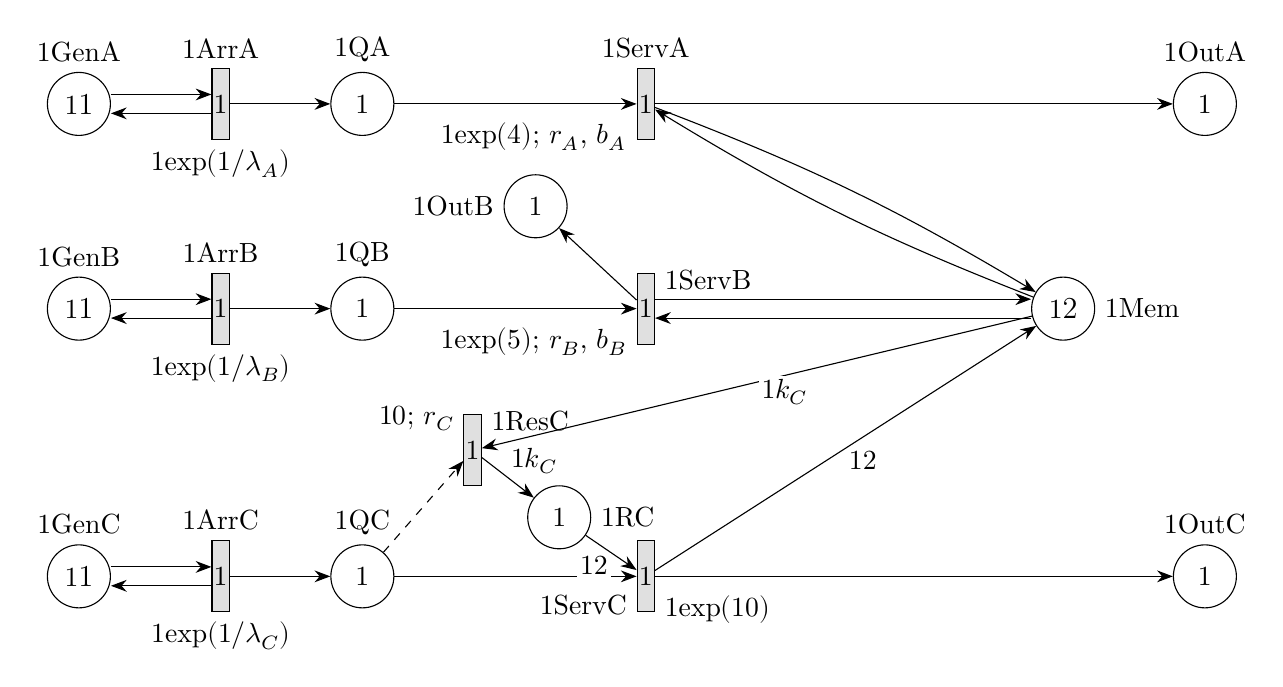
\begin{tikzpicture}[
    font=\setstretch{1}\fontsize{11}{13}\selectfont, >={Stealth[length=2mm]},
    pl/.style={draw, circle, minimum size=8mm, inner sep=0pt},
    tr/.style={draw, fill=black!12, rectangle, minimum width=2.2mm, minimum height=9mm, inner sep=0pt},
    arc/.style={->},
    rd/.style={->, dashed},
    nm/.style={font=\setstretch{1}\fontsize{10}{12}\selectfont},
    par/.style={font=\setstretch{1}\fontsize{10}{12}\selectfont, align=center},
    w/.style={font=\setstretch{1}\fontsize{10}{12}\selectfont, fill=white, inner sep=1pt},
  ]
  \def\yA{0} \def\yB{-2.6} \def\yC{-6.0}
  \def\xS{7.2}
  % Джерела та підчерги
  \foreach \i/\y/\l in {A/\yA/\lambda_A, B/\yB/\lambda_B, C/\yC/\lambda_C}{
    \node[pl, label={[nm]above:Gen\i}] (Gen\i) at (0,\y) {1};
    \node[tr, label={[nm]above:Arr\i}, label={[par]below:$\exp(1/\l)$}] (Arr\i) at (1.8,\y) {};
    \node[pl, label={[nm]above:Q\i}] (Q\i) at (3.6,\y) {};
    \draw[arc] ([yshift=1.2mm]Gen\i.east) -- ([yshift=1.2mm]Arr\i.west);
    \draw[arc] ([yshift=-1.2mm]Arr\i.west) -- ([yshift=-1.2mm]Gen\i.east);
    \draw[arc] (Arr\i) -- (Q\i);
  }
  % Виконання
  \node[tr, label={[nm]above:ServA}, label={[par]below left:$\exp(4)$; $r_A$, $b_A$}] (ServA) at (\xS,\yA) {};
  \node[tr, label={[nm]above right:ServB}, label={[par]below left:$\exp(5)$; $r_B$, $b_B$}] (ServB) at (\xS,\yB) {};
  \node[tr, label={[nm]below left:ServC}, label={[par]below right:$\exp(10)$}] (ServC) at (\xS,\yC) {};
  % Виходи
  \node[pl, label={[nm]above:OutA}] (OutA) at (14.3,\yA) {};
  \node[pl, label={[nm]left:OutB}] (OutB) at (5.8,-1.3) {};
  \node[pl, label={[nm]above:OutC}] (OutC) at (14.3,\yC) {};
  % Памʼять і резервування
  \node[pl, label={[nm]right:Mem}] (Mem) at (12.5,\yB) {2};
  \node[tr, label={[nm]above right:ResC}, label={[par]above left:$0$; $r_C$}] (ResC) at (5.0,-4.4) {};
  \node[pl, label={[nm]right:RC}] (RC) at (6.1,-5.25) {};
  % Дуги
  \draw[arc] (QA) -- (ServA);
  \draw[arc] (QB) -- (ServB);
  \draw[arc] (QC) -- (ServC);
  \draw[arc] (ServA) -- (OutA);
  \draw[arc] (ServB) -- (OutB);
  \draw[arc] (ServC) -- (OutC);
  \draw[arc] (Mem) to[bend left=5] (ServA);
  \draw[arc] (ServA) to[bend left=5] (Mem);
  \draw[arc] ([yshift=1.2mm]ServB.east) -- ([yshift=1.2mm]Mem.west);
  \draw[arc] ([yshift=-1.2mm]Mem.west) -- ([yshift=-1.2mm]ServB.east);
  \draw[arc] (Mem) -- node[w, pos=0.45, below] {$k_C$} (ResC);
  \draw[arc] (ResC) -- node[w, above right] {$k_C$} (RC);
  \draw[arc] (RC) -- node[w, below left] {2} (ServC);
  \draw[arc] (ServC) -- node[w, pos=0.5, below right] {2} (Mem);
  \draw[rd] (QC) -- (ResC);
\end{tikzpicture}

  \caption{Стохастична мережа Петрі інформаційної системи обробки завдань}
  \label{fig:petri}
\end{figure}

\begin{kpitable}{|c|L{12.4cm}|c|}{Позиції мережі Петрі та їх початкове маркірування~$m$\label{tab:places}}
  {\textbf{Позиція} & \textbf{Зміст} & \textbf{$m$}}
  Gen$i$ & умова роботи джерела типу~$i$ (маркер повертає перехід Arr$i$) & 1 \\ \hline
  Q$i$ & підчерга завдань типу~$i$ (кількість маркерів -- довжина підчерги) & 0 \\ \hline
  Mem & вільні одиниці оперативної памʼяті & $M=2$ \\ \hline
  RC & одиниці памʼяті, зарезервовані для завдання~C, що очікує & 0 \\ \hline
  Out$i$ & виконані завдання типу~$i$ (лічильник виходів із системи) & 0 \\ \hline
\end{kpitable}

\begin{kpitable}{|c|L{8.6cm}|L{2.6cm}|c|c|}{Переходи мережі Петрі\label{tab:transitions}}
  {\textbf{Перехід} & \textbf{Подія} & \textbf{$d$, хв} & \textbf{$r$} & \textbf{$b$}}
  ArrA & надходження завдання A & $\exp(5/\gamma)$ & 0 & 1 \\ \hline
  ArrB & надходження завдання B & $\exp(14{,}29/\gamma)$ & 0 & 1 \\ \hline
  ArrC & надходження завдання C & $\exp(16{,}67/\gamma)$ & 0 & 1 \\ \hline
  ServA & виконання завдання A & $\exp(4)$ & $r_A$ & $b_A$ \\ \hline
  ServB & виконання завдання B & $\exp(5)$ & $r_B$ & $b_B$ \\ \hline
  ResC & резервування памʼяті для завдання~C & 0 & $r_C$ & 1 \\ \hline
  ServC & виконання завдання C & $\exp(10)$ & 0 & 1 \\ \hline
\end{kpitable}

Затримки Arr$i$ задано через~$\gamma$ ($\lambda_i=\gamma\lambda_i^0$), Serv$i$ -- середніми $1/\mu_i$
з умови; $r_A$, $r_B$, $r_C$, $b_A$, $b_B$ і~$k_C$ залежать від стратегії (підрозділ~\ref{sec:strategies-net}).

Затримку $\exp(a)$ генерують методом оберненої функції~\cite{stetsenko-modeling}:
\[
  d = -a\ln(1-u), \qquad u \sim U[0;\,1),
\]
де $u$ -- псевдовипадкове число, $a = 1/\lambda_i$ для Arr$i$ і $1/\mu_i$ для Serv$i$. Якщо готові
кілька переходів з однаковим найвищим пріоритетом, генерують $u \sim U[0;\,1)$ і запускають перший
перехід $T_j$ групи, для якого $u < b_1 + \cdots + b_j$ (перехід з $b=1$ у групі з $n$ переходів
отримує ймовірність $1/n$).

Перехід Arr$i$ додає маркер у Q$i$. Перехід ServA (ServB) запускається за наявності маркерів у
QA (QB) і в Mem, утримує їх протягом виконання, повертає одиницю памʼяті в Mem і
передає завдання в OutA (OutB). Переходи виконання багатоканальні: за двох вільних одиниць
одночасно виконуються два завдання A/B (пари AA, AB, BB). ServC стартує лише тоді, коли для C
зарезервовано обидві одиниці (кратність дуги з~RC -- 2), і повертає їх у Mem після виконання;
поки виконується C, жодне інше завдання стартувати не може -- C монополізує систему.

Кількість завдань типу~$i$, що виконуються, дорівнює кількості активних каналів Serv$i$, і в
будь-який момент справджується інваріант памʼяті
\begin{equation}\label{eq:mem-invariant}
  m_{\text{Mem}} + m_{\text{RC}} + k_C\,n_{\text{ResC}} + n_{\text{ServA}} + n_{\text{ServB}}
    + 2\,n_{\text{ServC}} = M = 2,
\end{equation}
де $m_P$ -- кількість маркерів у позиції~$P$, $n_T$ -- кількість активних каналів переходу~$T$
(для ResC ненульова лише миттєво, бо $d=0$). Інваріант гарантує відсутність станів, заборонених
умовою, і використовується у верифікації (розділ~3).

\subsection{Відтворення стратегій упорядкування черги}\label{sec:strategies-net}

Пріоритет переходу визначає лише, яка з одночасно готових подій відбудеться першою. Цього
досить, щоб завдання вищого пріоритету першим займало памʼять, що звільнилася, але недостатньо
для правила резервування (підрозділ~\ref{sec:process}): коли завдання~C вищого пріоритету чекає двох вільних
одиниць памʼяті, а вільна лише одна, переходи ServA і ServB залишаються готовими і займали б її.
Тому до мережі додано перехід ResC і позицію RC. Перехід ResC готовий, поки в підчерзі QC є
завдання (інформаційна дуга) і в Mem є щонайменше $k_C$ вільних одиниць; запускаючись, він
переносить $k_C$ одиниць памʼяті в RC, де вони недоступні для A і~B. Отже, правило
резервування відтворено стандартними засобами формалізму: пріоритетом, кратністю дуг та
інформаційною дугою.

Параметри стратегій наведено в таблиці~\ref{tab:strategy-params} (більше~$r$ -- вищий пріоритет).

\needspace{10\baselineskip}
\begin{kpitable}{|c|c|c|c|c|c|c|}{Параметри мережі для стратегій упорядкування\label{tab:strategy-params}}
  {\textbf{$s$} & \textbf{Упорядкування} & \textbf{$r_A$} & \textbf{$r_B$} & \textbf{$r_C$} &
   \textbf{$k_C$} & \textbf{$b_A$; $b_B$}}
  1 & A $>$ B $>$ C   & 3 & 2 & 1 & 2 & 1; 1 \\ \hline
  2 & B $>$ A $>$ C   & 2 & 3 & 1 & 2 & 1; 1 \\ \hline
  3 & C $>$ B $>$ A   & 1 & 2 & 3 & 1 & 1; 1 \\ \hline
  4 & C $>$ A $>$ B   & 2 & 1 & 3 & 1 & 1; 1 \\ \hline
  5 & C $>$ (A $=$ B) & 1 & 1 & 2 & 1 & $0{,}5$; $0{,}5$ \\ \hline
\end{kpitable}

У стратегіях 3--5 перехід ResC має найвищий пріоритет і кратність $k_C=1$. Поки завдання~C
очікує, кожна одиниця памʼяті, що звільнилася, одразу резервується для нього, тому A і~B не
стартують навіть за наявності вільної одиниці; щойно в RC накопичуються дві одиниці, стартує
ServC. За інваріантом~\eqref{eq:mem-invariant} у RC не може бути більше двох маркерів. Якщо
завдання~C надходить за вільної памʼяті, ResC спрацьовує двічі в той самий момент часу і C
стартує без очікування.

У стратегіях 1--2 перехід ResC має найнижчий пріоритет і кратність $k_C=2$, тобто резервує
памʼять лише тоді, коли обидві одиниці вільні. Якби в цей момент у QA чи QB було завдання,
раніше спрацював би перехід ServA чи ServB з вищим пріоритетом, тому C стартує лише за порожніх
підчерг A і~B, як вимагає правило. Кратність $k_C=2$ тут обовʼязкова: за $k_C=1$ завдання~C
утримувало б одну одиницю, поки виконується інше завдання, і блокувало б A і~B, які
надходять пізніше, -- тобто отримало б фактичний пріоритет над ними.

Порядок A і~B задають $r_A$ і $r_B$; у стратегії~5 вони рівні, і конфлікт ServA і ServB за
вільну одиницю памʼяті розвʼязують ймовірності $b_A=b_B=0{,}5$; якщо готовий лише один із цих
переходів, він спрацьовує без розіграшу. Обслуговування без переривання
забезпечене тим, що запущений перехід утримує маркери до кінця затримки.

\subsection{Обчислення вихідних характеристик}

Статистику збирають на інтервалі $[T_{\text{п}};\,T_{\text{мод}}]$ тривалістю
$\tau=T_{\text{мод}}-T_{\text{п}}$. Якщо $t_j$ -- моменти подій, $\Delta t_j=t_{j+1}-t_j$, а
$m_P(t_j)$ і $n_T(t_j)$ -- стан протягом $j$-го інтервалу, то середні за часом
\begin{equation}\label{eq:time-means}
  \bar m_P = \frac{1}{\tau}\sum_j m_P(t_j)\,\Delta t_j, \qquad
  \bar n_T = \frac{1}{\tau}\sum_j n_T(t_j)\,\Delta t_j .
\end{equation}

Середня кількість завдань типу~$i$ у черзі та в системі, фактична інтенсивність надходження
($N_{\text{Arr}i}$ -- кількість спрацьовувань Arr$i$ за час~$\tau$) і, за законом
Літтла~\cite{kleinrock}, що для стаціонарного режиму не залежить від порядку обслуговування,
середні часи очікування й перебування:
\begin{equation}\label{eq:L-lambda}
  L_{q,i} = \bar m_{\text{Q}i}, \qquad
  L_i = \bar m_{\text{Q}i} + \bar n_{\text{Serv}i}, \qquad
  \hat\lambda_i = \frac{N_{\text{Arr}i}}{\tau}.
\end{equation}
\begin{equation}\label{eq:W-type}
  W_{q,i} = \frac{L_{q,i}}{\hat\lambda_i}, \qquad W_i = \frac{L_i}{\hat\lambda_i}.
\end{equation}
Загальні показники -- середні за всіма завданнями, тобто зважені за кількістю завдань кожного
типу (для $W$ маємо $\sum_i \hat\lambda_i W_i / \sum_i \hat\lambda_i = \sum_i L_i/\sum_i\hat\lambda_i$),
а допоміжний коефіцієнт використання памʼяті~\eqref{eq:U} -- частка зайнятих одиниць без
зарезервованих:
\begin{equation}\label{eq:W-total}
  L_q = \sum_{i} L_{q,i}, \qquad
  W_q = \frac{\sum_i L_{q,i}}{\sum_i \hat\lambda_i}, \qquad
  W = \frac{\sum_i L_i}{\sum_i \hat\lambda_i}.
\end{equation}
\begin{equation}\label{eq:U}
  U = \frac{\bar n_{\text{ServA}} + \bar n_{\text{ServB}} + 2\,\bar n_{\text{ServC}}}{M}
    = 1 - \frac{\bar m_{\text{Mem}} + \bar m_{\text{RC}}}{M}.
\end{equation}
Друга рівність випливає з інваріанту~\eqref{eq:mem-invariant}; $\bar m_{\text{RC}}/M$ -- частка
памʼяті, що простоює через резервування. Формули~\eqref{eq:time-means}--\eqref{eq:W-total} дають
саме ті характеристики, які названо в умові задачі: середній час перебування завдання в системі
($W$, $W_i$), середню кількість завдань у черзі ($L_q$, $L_{q,i}$) і середній час очікування в
черзі ($W_q$, $W_{q,i}$). Вони мають сенс лише за стійкого режиму, коли довжини черг не
зростають необмежено; кожну оцінюють як середнє
за $p$ прогонами з точністю 2~\% середнього і довірчою ймовірністю 0,95 (підрозділ~\ref{sec:exp-runs}).

\subsection{Висновки до розділу}

Систему формалізовано стохастичною мережею Петрі з 11 позицій і 7 переходів: обмеження на
одночасне виконання відтворено позицією памʼяті й кратністю дуг, стратегії -- пріоритетами,
ймовірностями запуску й кратністю дуги резервування, правило резервування -- переходом ResC з
інформаційною дугою. Наведено генератори, формули відгуків і інваріант памʼяті.

\section{Алгоритмізація та програмна реалізація імітаційної моделі системи}

\subsection{Вибір засобів програмної реалізації}

Модель реалізовано мовою Java~\cite{java-jls} (версія мови~23) із системою збирання
Maven~\cite{maven}. По-перше, мовою Java написане ядро PetriObjModelPaint~\cite{petriobjmodelpaint}
(модуль \texttt{petri-math}), у якому реалізовано алгоритм імітації стохастичної мережі Петрі за
посібником~\cite{stetsenko-kursova,stetsenko-modeling}: програма підключає його як бібліотеку, тож
алгоритм імітації й семантика елементів мережі залишаються такими самими, як у ядрі. По-друге,
наслідування з перевизначенням методів дає змогу внести потрібні задачі зміни в класах-нащадках,
не змінюючи коду ядра. По-третє,
генератори з заданим seed (\texttt{SplittableRandom}~\cite{java-api}) забезпечують відтворюваність
прогонів, а скомпільована програма працює швидко: серія прогонів верифікації (понад
$4{,}8\cdot10^8$ подій) триває близько 11~с. Недолік Java -- бідніші, ніж у Python, засоби
статистичної обробки й побудови графіків, тому результати експериментів оброблено мовою Python
(розділ~4).

З ядра використано класи \texttt{PetriP}, \texttt{PetriT}, \texttt{ArcIn}, \texttt{ArcOut},
\texttt{PetriNet}, \texttt{PetriSim} з процедурами входу (\texttt{input}) і виходу маркерів
(\texttt{output}) та пошуку найближчої події (\texttt{eventMin}); вихідний код ядра не змінювався,
модифікації внесено в класах-нащадках (таблиця~\ref{tab:kernel-mods}). Ядро універсальне, тому
його використання пристосовано до задачі. Модель -- одна мережа Петрі,
тож замість циклу \texttt{PetriObjModel.go}, що на кожній події перемішує й сортує Петрі-обʼєкти
(це потрібно лише для спільних позицій кількох обʼєктів), і методу \texttt{PetriSim.go}, що друкує
маркірування на кожному кроці, працює власний цикл однієї мережі (алгоритм~\ref{alg:main}).
Решту засобів ядра задача потребує: пріоритети (стратегії 1--4), імовірності запуску (стратегія~5),
багатоканальні переходи (пари AA, AB, BB), кратні та інформаційну дуги (резервування памʼяті), тому
їх не вилучено. Натомість пошук активних переходів
\texttt{findActiveT}, на який припадає найбільше часу, перевизначено: ядро після кожного запуску
перевіряє всі переходи за списками \texttt{Integer} і сортує активні, а в \texttt{PetriSimulator}
переходи впорядковано за пріоритетом один раз до прогону й вхідні дуги зведено в масиви. Результат
той самий, а прогін у 1,25--1,28~раза швидший, ніж циклом
\texttt{PetriObjModel.go}.

\begin{kpitable}{|L{3.4cm}|L{4.8cm}|L{7.4cm}|}{Модифікації ядра PetriObjModelPaint\label{tab:kernel-mods}}
  {\textbf{Що змінено} & \textbf{В ядрі PetriObjModelPaint} & \textbf{Розширення в програмі моделі та обґрунтування}}
  Затримка переходу & метод \texttt{getTimeServ} класу \texttt{PetriT}: закон -- рядком, значення -- \texttt{FunRand}
    на основі \texttt{Math.random()} & \texttt{StochasticTransition}: затримка -- обʼєкт \texttt{Delay},
    значення -- з генератора прогону із заданим seed (прогін відтворюється точно) \\ \hline
  Вирішення конфлікту & метод \texttt{doConflikt} класу \texttt{PetriSim} на основі \texttt{Math.random()} &
    \texttt{PetriSimulator}: те саме правило (\texttt{ConflictResolver}) з генератором прогону \\ \hline
  Середні значення & \texttt{getMean} з вагою $\Delta t/t'$, тобто від моменту~0 &
    \texttt{PetriSimulator.run} викликає \texttt{doStatistics} ядра з вагою
    $\Delta t/(t'-T_{\text{п}})$: середні~\eqref{eq:time-means} лише на $[T_{\text{п}};\,T_{\text{мод}}]$ \\ \hline
  Лічильники спрацьовувань & відсутні & \texttt{StochasticTransition}: лічильники запусків і
    завершень, обнулення в момент~$T_{\text{п}}$; потрібні для $N_{\text{Arr}i}$ у формулі~\eqref{eq:L-lambda} \\ \hline
  Нумерація елементів & статичний лічильник класу, має збігатися з індексом у мережі &
    \texttt{PetriNetBuilder}: явні номери й перевірка структури мережі \\ \hline
  Спостереження за станом & один спостерігач фаз переходу & \texttt{PetriSimulator}: стан після
    кожної події -- спостерігачам \texttt{SimulationListener} (інваріанти, протокол подій) \\ \hline
  Цикл імітації і пошук активних переходів & \texttt{PetriObjModel.go} перемішує й сортує Петрі-обʼєкти
    на кожній події; \texttt{findActiveT} перевіряє всі переходи й сортує активні &
    \texttt{PetriSimulator}: цикл однієї мережі; переходи впорядковано за~$r$ один раз до прогону,
    вхідні дуги -- у масивах (той самий результат, прогін у 1,25--1,28~раза швидший) \\ \hline
\end{kpitable}

\subsection{Алгоритм імітації стохастичної мережі Петрі}

Алгоритм імітації подієвий: модельний час просувається до найближчого моменту виходу маркерів
з переходу. Стан мережі -- маркірування позицій і множина активних каналів переходів із
моментами їх завершення; кожен запуск відкриває новий канал, вилучаючи маркери з вхідних позицій
(крім інформаційних дуг), а у вихідні позиції маркери надходять через затримку~$d$
(алгоритм~\ref{alg:main}).

\begin{algorithm}[tp]
  \caption{Імітація стохастичної мережі Петрі}\label{alg:main}
  \begin{algorithmic}[1]
    \Require мережа в початковому маркіруванні, $T_{\text{мод}}$, $T_{\text{п}}$, seed генератора
    \State $t \gets 0$; якщо $T_{\text{п}} = 0$, розпочати збір статистики
    \State \Call{ВхідМаркерів}{$t$}
    \Loop
      \State $t' \gets \min_T \min_j t^{\text{вих}}_{T,j}$
      \If{$t' > T_{\text{мод}}$}
        \State \Call{ПросуванняЧасу}{$T_{\text{мод}}$}; \textbf{завершити}
      \EndIf
      \State \Call{ПросуванняЧасу}{$t'$}
      \ForAll{канали $j$ переходів $T$, де $t^{\text{вих}}_{T,j} = t$}
        \State вихід маркерів з каналу $j$: $m_P \gets m_P + k$ для дуг $(T, P, k)$
      \EndFor
      \State \Call{ВхідМаркерів}{$t$}; повідомити спостерігачів про новий стан
    \EndLoop
    \Statex
    \Procedure{ПросуванняЧасу}{$t'$}
      \If{статистика не збирається \textbf{і} $t' \ge T_{\text{п}}$}
        \State $t \gets T_{\text{п}}$; розпочати збір статистики; обнулити лічильники
      \EndIf
      \If{статистика збирається}
        \State $a \gets (t'-t)/(t'-T_{\text{п}})$
        \State для кожної позиції $P$: $\bar m_P \gets \bar m_P + (m_P-\bar m_P)\,a$
        \State для кожного переходу $T$: $\bar n_T \gets \bar n_T + (n_T-\bar n_T)\,a$
      \EndIf
      \State $t \gets t'$
    \EndProcedure
  \end{algorithmic}
\end{algorithm}

Просування стану складається з двох фаз: вихід маркерів з каналів, що завершуються в момент~$t$,
і запуск переходів, умова запуску яких виконана (алгоритм~\ref{alg:input}). Тут реалізовано
пріоритети й імовірності запуску з таблиці~\ref{tab:strategy-params}: запускається один перехід
з найвищим~$r$ (за кількох -- обраний випадково з імовірностями~$b$), після чого умови
перераховуються. Канал ResC ($d=0$) завершується в той самий момент, тож памʼять потрапляє в RC на
наступній ітерації без просування часу.

\begin{algorithm}[tp]
  \caption{Вхід маркерів у переходи з вирішенням конфліктів}\label{alg:input}
  \begin{algorithmic}[1]
    \Procedure{ВхідМаркерів}{$t$}
      \State $\mathcal{A} \gets \{T : b_T \neq 0 \text{ і } m_P \ge k \text{ для кожної вхідної дуги } (P, T, k)\}$
      \While{$\mathcal{A} \neq \emptyset$}
        \State упорядкувати $\mathcal{A}$ за спаданням $r$; $\mathcal{G}$ -- переходи з найвищим $r$
        \If{$|\mathcal{G}| = 1$}
          \State $T^* \gets$ єдиний перехід групи $\mathcal{G}$
        \Else
          \State $u \gets U[0;1)$; $T^* \gets$ перший $T \in \mathcal{G}$, для якого
            $\sum p_T > u$, де $p_T = b_T$, якщо $b_T < 1$, інакше $p_T = 1/|\mathcal{G}|$
        \EndIf
        \State $m_P \gets m_P - k$ для кожної вхідної дуги $(P, T^*, k)$, крім інформаційних
        \State відкрити канал $T^*$ з моментом виходу $t + d_{T^*}$, $d_{T^*}$ -- реалізація затримки
        \State перерахувати $\mathcal{A}$
      \EndWhile
    \EndProcedure
  \end{algorithmic}
\end{algorithm}

Між двома подіями стан не змінюється, тому рекурентна формула з вагою $a=(t'-t)/(t'-T_{\text{п}})$
дає точне середнє за часом на $[T_{\text{п}};\,t']$, а наприкінці прогону -- середні~\eqref{eq:time-means};
перший крок після $T_{\text{п}}$ має вагу $a=1$, тож середнє починається зі стану в момент~$T_{\text{п}}$. Потім
відгуки обчислюються за формулами~\eqref{eq:L-lambda}--\eqref{eq:U}.

\subsection{Структура програми}\label{sec:structure}

Програму поділено на пакети: \texttt{petri} -- розширення ядра (не залежить від задачі B14),
\texttt{model} -- модель системи B14, \texttt{verification} -- засоби верифікації,
\texttt{experiment} -- серії прогонів розділу~4, \texttt{io} і \texttt{app} -- файли CSV і запуск з
командного рядка. Залежності між пакетами спрямовані до пакета \texttt{petri}, а від нього -- до
бібліотеки ядра, тому розширення ядра перевіряється окремо від моделі. Призначення основних класів
наведено в таблиці~\ref{tab:classes}.

\begin{kpitable}{|L{5.9cm}|L{9.7cm}|}{Призначення основних класів програми\label{tab:classes}}
  {\textbf{Клас} & \textbf{Призначення}}
  \texttt{StochasticTransition} & нащадок \texttt{PetriT}: затримка з генератора прогону, лічильники \\ \hline
  \texttt{PetriSimulator} & нащадок \texttt{PetriSim}: алгоритми~\ref{alg:main} і~\ref{alg:input}, статистика після $T_{\text{п}}$ \\ \hline
  \texttt{PetriNetBuilder} & побудова й перевірка мережі \texttt{PetriNet} з елементів ядра \\ \hline
  \texttt{Strategy} & $r_A$, $r_B$, $r_C$, $k_C$, $b_A$, $b_B$ стратегій (таблиця~\ref{tab:strategy-params}) \\ \hline
  \texttt{ModelParameters} & вхідні змінні $s$, $\lambda_i$ ($\gamma\lambda_i^0$), а також $1/\mu_i$ і~$M$ \\ \hline
  \texttt{B14Net} & мережа рисунка~\ref{fig:petri}, ліва частина інваріанту~\eqref{eq:mem-invariant} \\ \hline
  \texttt{OutputCalculator} & відгуки за формулами~\eqref{eq:L-lambda}--\eqref{eq:U} \\ \hline
  \texttt{B14Simulation} & один прогін: мережа, генератор, імітація, відгуки \\ \hline
  \texttt{InvariantMonitor} & перевірка інваріанту й правил упорядкування після кожної події \\ \hline
  \texttt{VerificationRunner} & серії верифікації, зокрема порівняння з M/M/$c$ (\texttt{MmcQueue}) \\ \hline
  \texttt{ResponseTrajectory} & середні відгуки на $[0;\,t]$ і поточна черга (вибір $T_{\text{п}}$, $T_{\text{мод}}$) \\ \hline
  \texttt{ExperimentRunner} & серії прогонів експериментального дослідження \\ \hline
\end{kpitable}

Мережу будує клас \texttt{B14Net}; назви позицій і переходів збігаються з рисунком~\ref{fig:petri},
стратегію задають лише параметри переходів ResC і Serv$i$, тож структура мережі однакова для всіх
стратегій. Фрагмент побудови цих переходів
(початкова версія -- модель за умовою задачі; зміни для пропозиції -- у
підрозділі~\ref{sec:improvement}):
\begin{Verbatim}[gobble=8]
        int kC = strategy.reservationMultiplicity();
        reservationMultiplicity = kC;
        reservation = builder.transition(RESERVE_C).delay(Delay.constant(0))
                .priority(strategy.priority(TaskType.C))
                .informationalInput(queues.get(TaskType.C), 1)
                .input(memory, kC).output(reserved, kC).add();

        for (TaskType type : TaskType.values()) {
            PetriP done = builder.place("Out" + type, 0);
            PetriP resource = type == TaskType.C ? reserved : memory;
            int v = type.memoryDemand();
            int priority = type == TaskType.C ? 0 : strategy.priority(type);
            services.put(type, builder.transition(serviceName(type))
                    .delay(Delay.exponential(parameters.meanServiceTime(type)))
                    .priority(priority).probability(strategy.launchProbability(type))
                    .input(queues.get(type)).input(resource, v)
                    .output(memory, v).output(done).add());
        }
\end{Verbatim}

Звʼязки між класами, їх поля й методи показано на UML-діаграмі (рисунок~\ref{fig:uml}).

\begin{figure}
  \centering
  % Рисунок 3.1 — UML-діаграма класів програми (sim/, пакет ua.kpi.km.b14).
% Члени класів скорочено до тих, що потрібні для розуміння алгоритму:
% «+» — public, «-» — private, «~» — доступ у межах пакета.
% Пакет petri-math — бібліотека ядра (без змін); методи, показані в нащадках
% (StochasticTransition, PetriSimulator), перевизначають однойменні методи ядра.
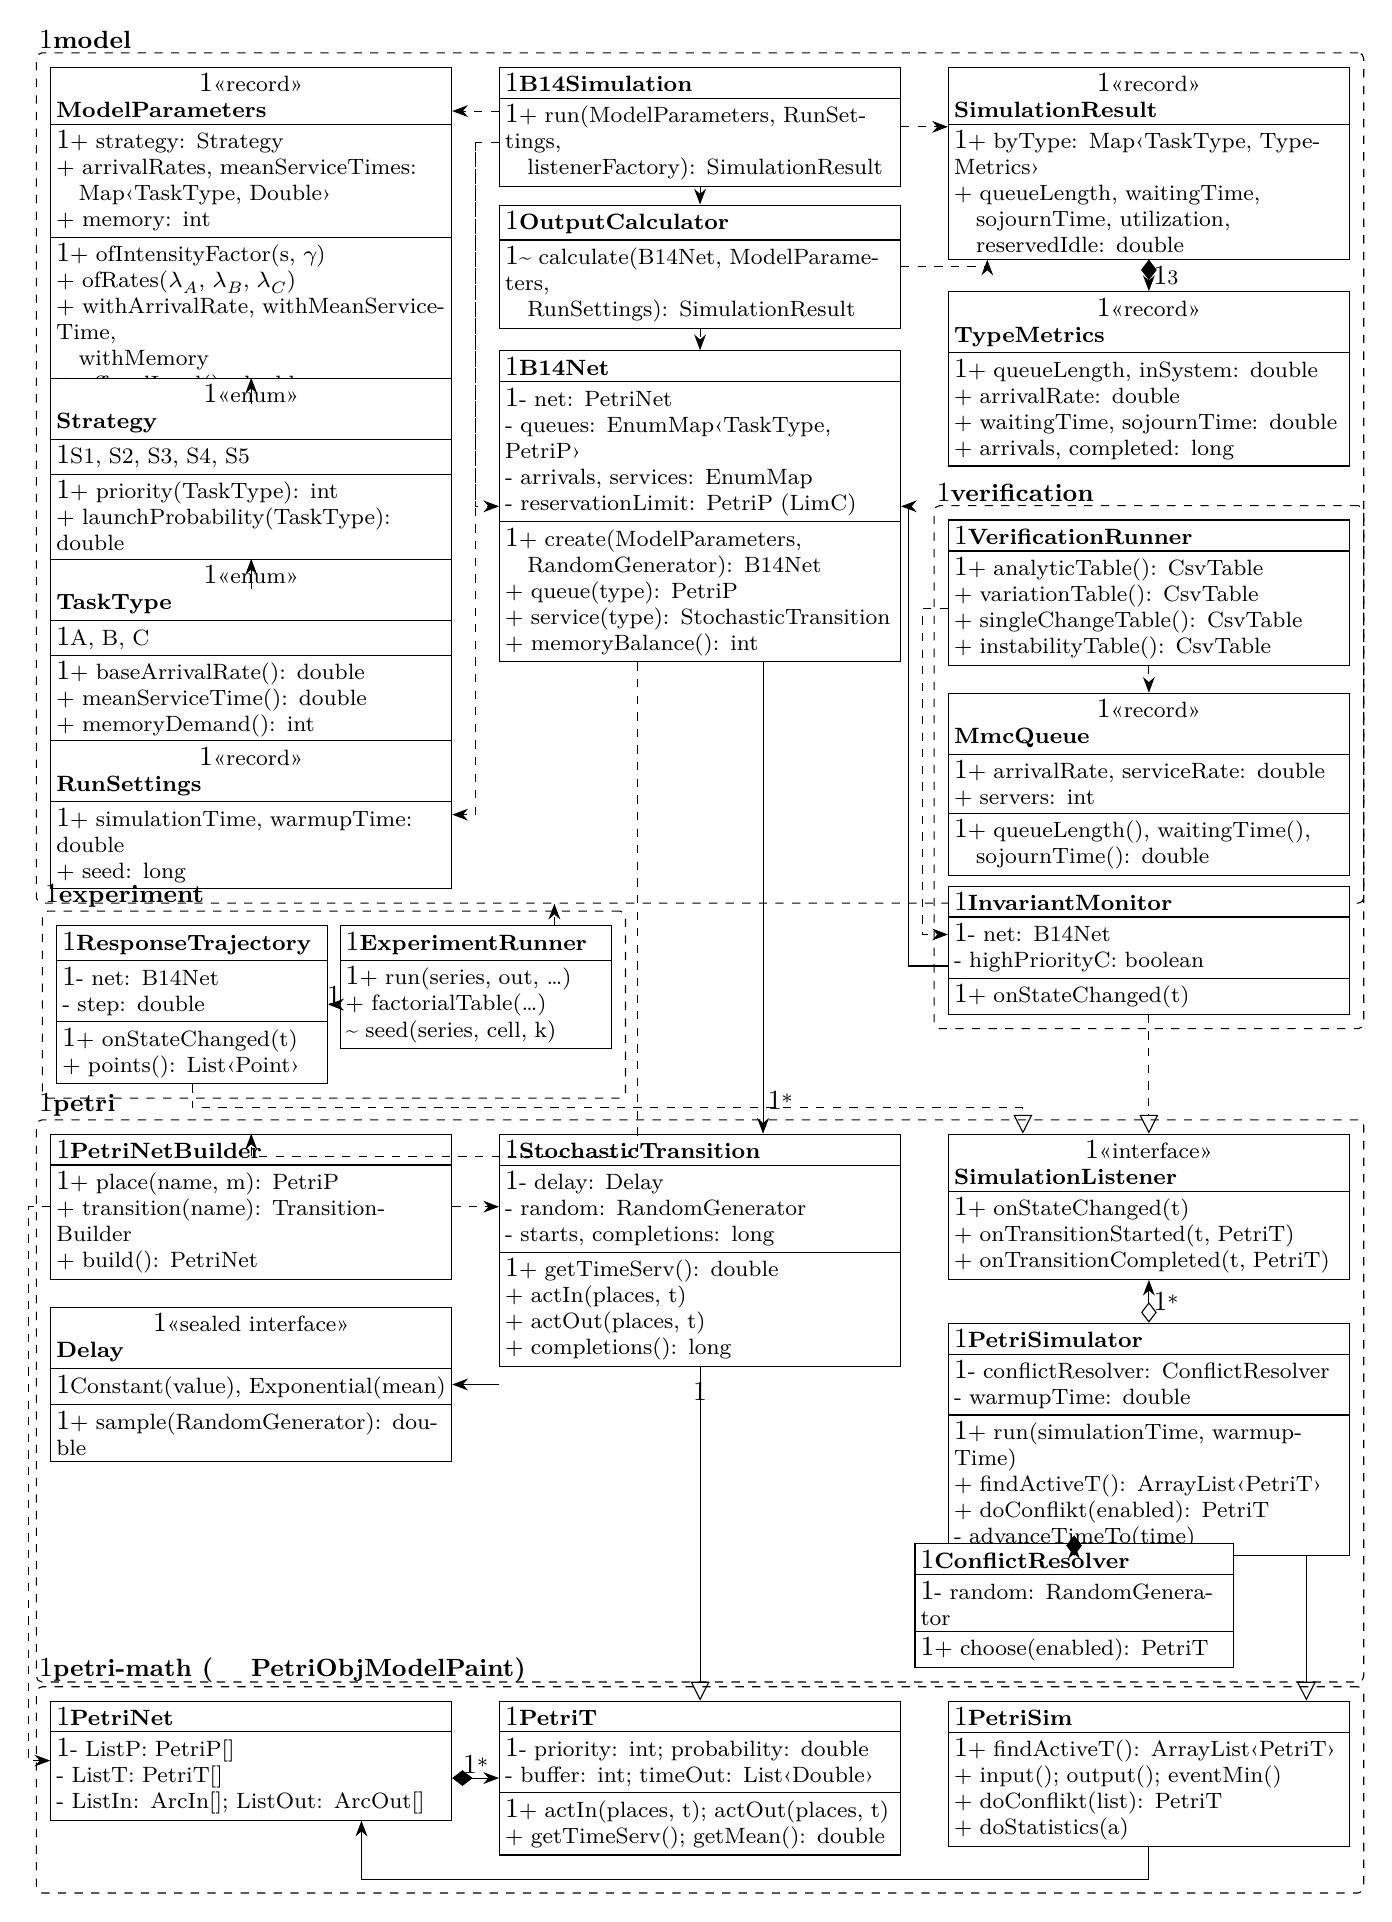
\begin{tikzpicture}[
    font=\setstretch{1}\fontsize{8}{9.4}\selectfont,
    uml/.style={draw, fill=white, rectangle split, rectangle split parts=3,
      rectangle split ignore empty parts, rectangle split part align={center,left,left},
      text width=4.95cm, inner sep=2pt, anchor=north},
    pkg/.style={draw, dashed, rounded corners=2pt, inner sep=5pt},
    pkgname/.style={anchor=south west, inner sep=1pt,
      font=\setstretch{1}\fontsize{9}{11}\selectfont\bfseries},
    dep/.style={-{Stealth[length=2mm]}, dashed},
    assoc/.style={-{Stealth[length=2mm]}},
    comp/.style={{Diamond[length=2.6mm, width=2mm]}-{Stealth[length=2mm]}},
    agg/.style={{Diamond[open, length=2.6mm, width=2mm]}-{Stealth[length=2mm]}},
    real/.style={-{Triangle[open, length=2.4mm, width=2.4mm]}, dashed},
    inherit/.style={-{Triangle[open, length=2.4mm, width=2.4mm]}},
    ml/.style={font=\setstretch{1}\fontsize{7.5}{9}\selectfont, inner sep=1.5pt},
  ]
  \def\xa{0} \def\xb{5.7} \def\xc{11.4}
  \newcommand\tld{\textasciitilde}

  % ---------------- пакет model ----------------
  \node[uml] (Params) at (\xa,0) {\centering «record»\\\textbf{ModelParameters}
    \nodepart{second}+ strategy: Strategy\\+ arrivalRates, meanServiceTimes:\\\quad Map‹TaskType, Double›\\+ memory: int
    \nodepart{third}+ ofIntensityFactor(s, $\gamma$)\\+ ofRates($\lambda_A$, $\lambda_B$, $\lambda_C$)\\+ withArrivalRate, withMeanServiceTime,\\\quad withMemory\\+ offeredLoad(): double};
  \node[uml] (Strategy) at (\xa,-3.95) {\centering «enum»\\\textbf{Strategy}
    \nodepart{second}S1, S2, S3, S4, S5
    \nodepart{third}+ priority(TaskType): int\\+ launchProbability(TaskType): double\\+ reservationMultiplicity(): int};
  \node[uml] (TaskType) at (\xa,-6.25) {\centering «enum»\\\textbf{TaskType}
    \nodepart{second}A, B, C
    \nodepart{third}+ baseArrivalRate(): double\\+ meanServiceTime(): double\\+ memoryDemand(): int};
  \node[uml] (Settings) at (\xa,-8.55) {\centering «record»\\\textbf{RunSettings}
    \nodepart{second}+ simulationTime, warmupTime: double\\+ seed: long};

  \node[uml] (Sim) at (\xb,0) {\centering \textbf{B14Simulation}
    \nodepart{third}+ run(ModelParameters, RunSettings,\\\quad listenerFactory): SimulationResult};
  \node[uml] (Calc) at (\xb,-1.75) {\centering \textbf{OutputCalculator}
    \nodepart{third}\tld{} calculate(B14Net, ModelParameters,\\\quad RunSettings): SimulationResult};
  \node[uml] (Net) at (\xb,-3.6) {\centering \textbf{B14Net}
    \nodepart{second}- net: PetriNet\\- queues: EnumMap‹TaskType, PetriP›\\- arrivals, services: EnumMap\\- reservationLimit: PetriP (LimC)
    \nodepart{third}+ create(ModelParameters,\\\quad RandomGenerator): B14Net\\+ queue(type): PetriP\\+ service(type): StochasticTransition\\+ memoryBalance(): int};

  \node[uml] (Result) at (\xc,0) {\centering «record»\\\textbf{SimulationResult}
    \nodepart{second}+ byType: Map‹TaskType, TypeMetrics›\\+ queueLength, waitingTime,\\\quad sojournTime, utilization,\\\quad reservedIdle: double};
  \node[uml] (Metrics) at (\xc,-2.85) {\centering «record»\\\textbf{TypeMetrics}
    \nodepart{second}+ queueLength, inSystem: double\\+ arrivalRate: double\\+ waitingTime, sojournTime: double\\+ arrivals, completed: long};

  % ---------------- пакет verification ----------------
  \node[uml] (Runner) at (\xc,-5.75) {\centering \textbf{VerificationRunner}
    \nodepart{third}+ analyticTable(): CsvTable\\+ variationTable(): CsvTable\\+ singleChangeTable(): CsvTable\\+ instabilityTable(): CsvTable};
  \node[uml] (Mmc) at (\xc,-7.95) {\centering «record»\\\textbf{MmcQueue}
    \nodepart{second}+ arrivalRate, serviceRate: double\\+ servers: int
    \nodepart{third}+ queueLength(), waitingTime(),\\\quad sojournTime(): double};
  \node[uml] (Monitor) at (\xc,-10.4) {\centering \textbf{InvariantMonitor}
    \nodepart{second}- net: B14Net\\- highPriorityC: boolean
    \nodepart{third}+ onStateChanged(t)};

  % ---------------- пакет petri ----------------
  \node[uml] (Listener) at (\xc,-13.55) {\centering «interface»\\\textbf{SimulationListener}
    \nodepart{third}+ onStateChanged(t)\\+ onTransitionStarted(t, PetriT)\\+ onTransitionCompleted(t, PetriT)};
  \node[uml] (Simulator) at (\xc,-15.95) {\centering \textbf{PetriSimulator}
    \nodepart{second}- conflictResolver: ConflictResolver\\- warmupTime: double
    \nodepart{third}+ run(simulationTime, warmupTime)\\+ findActiveT(): ArrayList‹PetriT›\\+ doConflikt(enabled): PetriT\\- advanceTimeTo(time)};
  \node[uml, text width=3.9cm] (Resolver) at (\xc-0.95,-18.75) {\centering \textbf{ConflictResolver}
    \nodepart{second}- random: RandomGenerator
    \nodepart{third}+ choose(enabled): PetriT};

  \node[uml] (STrans) at (\xb,-13.55) {\centering \textbf{StochasticTransition}
    \nodepart{second}- delay: Delay\\- random: RandomGenerator\\- starts, completions: long
    \nodepart{third}+ getTimeServ(): double\\+ actIn(places, t)\\+ actOut(places, t)\\+ completions(): long};

  \node[uml] (Builder) at (\xa,-13.55) {\centering \textbf{PetriNetBuilder}
    \nodepart{third}+ place(name, m): PetriP\\+ transition(name): TransitionBuilder\\+ build(): PetriNet};
  \node[uml] (Delay) at (\xa,-15.75) {\centering «sealed interface»\\\textbf{Delay}
    \nodepart{second}Constant(value), Exponential(mean)
    \nodepart{third}+ sample(RandomGenerator): double};

  % ---------------- пакет experiment (розділ 4) ----------------
  \node[uml, text width=3.3cm] (Traj) at (-0.75,-10.9) {\centering \textbf{ResponseTrajectory}
    \nodepart{second}- net: B14Net\\- step: double
    \nodepart{third}+ onStateChanged(t)\\+ points(): List‹Point›};
  \node[uml, text width=3.3cm] (Exp) at (2.85,-10.9) {\centering \textbf{ExperimentRunner}
    \nodepart{third}+ run(series, out, \ldots)\\+ factorialTable(\ldots)\\\tld{} seed(series, cell, k)};

  % ---------------- бібліотека petri-math (ядро) ----------------
  \node[uml] (KNet) at (\xa,-20.75) {\centering \textbf{PetriNet}
    \nodepart{second}- ListP: PetriP[]\\- ListT: PetriT[]\\- ListIn: ArcIn[]; ListOut: ArcOut[]};
  \node[uml] (KT) at (\xb,-20.75) {\centering \textbf{PetriT}
    \nodepart{second}- priority: int; probability: double\\- buffer: int; timeOut: List‹Double›
    \nodepart{third}+ actIn(places, t); actOut(places, t)\\+ getTimeServ(); getMean(): double};
  \node[uml] (KSim) at (\xc,-20.75) {\centering \textbf{PetriSim}
    \nodepart{third}+ findActiveT(): ArrayList‹PetriT›\\+ input(); output(); eventMin()\\+ doConflikt(list): PetriT\\+ doStatistics(a)};

  \coordinate (k2) at ($(KT.south)+(0,-0.3)$); % траса асоціації PetriSim -> PetriNet

  % ---------------- рамки пакетів ----------------
  \begin{scope}[on background layer]
    \node[pkg, fit=(Params)(Settings)(Sim)(Net)(Result)(Metrics)] (Pmodel) {};
    \node[pkg, fit=(Runner)(Mmc)(Monitor)] (Pver) {};
    \node[pkg, fit=(Builder)(Delay)(STrans)(Listener)(Resolver)] (Ppetri) {};
    \node[pkg, fit=(KNet)(KT)(KSim)(k2)] (Pkernel) {};
    \node[pkg, fit=(Traj)(Exp)] (Pexp) {};
  \end{scope}
  \node[pkgname] at (Pmodel.north west) {model};
  \node[pkgname] at (Pver.north west) {verification};
  \node[pkgname] at (Ppetri.north west) {petri};
  \node[pkgname] at (Pkernel.north west) {petri-math (ядро PetriObjModelPaint)};
  \node[pkgname] at (Pexp.north west) {experiment};

  % ---------------- зв'язки ----------------
  % model
  \draw[assoc] (Params) -- (Strategy);
  \draw[assoc] (Strategy) -- (TaskType);
  \coordinate (s1) at ([yshift=2mm]Sim.west);
  \draw[dep] (s1) -- (Params.east |- s1);
  \coordinate (g1) at ($([yshift=-2mm]Sim.west)+(-0.3,0)$);
  \draw[dep] ([yshift=-2mm]Sim.west) -- (g1) |- (Net.west);
  \draw[dep] (g1) |- (Settings.east);
  \draw[dep] (Sim) -- (Calc);
  \draw[dep] (Calc) -- (Net);
  \draw[dep] (Sim.east) -- (Result.west |- Sim.east);
  \draw[dep] (Calc.east) -| ($(Result.south west)+(0.5,0)$);
  \draw[comp] (Result) -- node[ml, right]{3} (Metrics);
  % verification
  \draw[dep] (Runner) -- (Mmc);
  \draw[dep] ([yshift=-2mm]Runner.west) -- ++(-0.32,0) |- ([yshift=2mm]Monitor.west);
  \draw[assoc] ([yshift=-2mm]Monitor.west) -- ++(-0.5,0) |- (Net.east);
  \draw[real] (Monitor) -- (Listener);
  % petri
  \draw[assoc] ([xshift=0.8cm]Net.south) -- node[ml, right, pos=0.93]{*} ([xshift=0.8cm]Net.south |- STrans.north);
  \coordinate (b1) at ($([xshift=-0.8cm]Net.south)+(0,-6.27)$);
  \draw[dep] ([xshift=-0.8cm]Net.south) -- (b1) -| (Builder.north);
  \draw[dep] (Builder.east) -- (Builder.east -| STrans.west);
  \draw[assoc] (STrans.west |- Delay.east) -- (Delay.east);
  \draw[agg] (Simulator) -- node[ml, right]{*} (Listener);
  \draw[comp] (Resolver.north |- Simulator.south) -- (Resolver.north);
  % experiment: залежність від пакета model (B14Simulation, ModelParameters, RunSettings)
  \draw[dep] (Exp.west |- Traj.east) -- (Traj.east);
  \draw[dep] ([xshift=1.0cm]Exp.north) -- ([xshift=1.0cm]Exp.north |- Pmodel.south);
  \draw[real] (Traj.south) -- ++(0,-0.3) -| ([xshift=-1.6cm]Listener.north);
  % наслідування від класів ядра
  \draw[inherit] (STrans) -- (KT);
  \draw[inherit] ([xshift=2.0cm]Simulator.south) -- ([xshift=2.0cm]Simulator.south |- KSim.north);
  % petri-math
  \coordinate (k1) at ($(Builder.west)+(-0.28,0)$);
  \draw[dep] (Builder.west) -- (k1) |- (KNet.west);
  \draw[comp] (KNet.east |- KT.west) -- node[ml, above]{*} (KT.west);
  \draw[assoc] (KSim.south) -- (KSim.south |- k2) -| ([xshift=1.4cm]KNet.south);
\end{tikzpicture}

  \caption{UML-діаграма класів програми}
  \label{fig:uml}
\end{figure}

Клас \texttt{StochasticTransition} генерує затримку законом \texttt{Delay} і оновлює лічильники
після виклику методу ядра, лише якщо кількість активних каналів змінилася:
\codeinput[firstline=46, lastline=72, gobble=4]{../sim/src/main/java/ua/kpi/km/b14/petri/StochasticTransition.java}

У методі просування часу класу \texttt{PetriSimulator} в момент~$T_{\text{п}}$ обнуляються
лічильники, а вага методу ядра \texttt{doStatistics} відлічується від~$T_{\text{п}}$:
\codeinput[firstline=124, lastline=152, gobble=4]{../sim/src/main/java/ua/kpi/km/b14/petri/PetriSimulator.java}

Клас \texttt{ConflictResolver} відтворює правило ядра: перехід з $b=1$ у групі з $n$
рівнопріоритетних отримує ймовірність $1/n$, інший -- свою~$b$ (у стратегії~5 -- по~0,5):
\codeinput[firstline=36, lastline=52, gobble=4]{../sim/src/main/java/ua/kpi/km/b14/petri/ConflictResolver.java}

Клас \texttt{OutputCalculator} обчислює відгуки за формулами~\eqref{eq:L-lambda}
і~\eqref{eq:W-type}:
\codeinput[firstline=28, lastline=44, gobble=8]{../sim/src/main/java/ua/kpi/km/b14/model/OutputCalculator.java}

Програму запускають з командного рядка (команди \texttt{run}, \texttt{verify},
\texttt{experiment}). Програму перевірено 42~тестами JUnit~5~\cite{junit}, головні -- тести
еквівалентності розширення ядра: мережа з пріоритетами, кратними й інформаційною дугами та багатоканальними
переходами дає ті самі маркірування й середні в циклі \texttt{PetriObjModel.go} ядра і в
\texttt{PetriSimulator}, а \texttt{findActiveT} у мережі B14 -- той самий список, що й ядро. Інші
тести перевіряють точні лічильники й середні для мережі з детермінованими затримками, початок
статистики після~$T_{\text{п}}$, перевагу пріоритету, невилучення маркерів інформаційною дугою,
частоти вибору за ймовірностями запуску, відтворюваність прогону з тим самим seed і нумерацію
елементів незалежно від лічильників ядра. Текст
основних класів наведено в додатку~А (ядра -- у~\cite{petriobjmodelpaint}), засобів верифікації --
у додатку~В. Повний вихідний код програми, скриптів аналізу, мережу Петрі у форматі PNML і
результати прогонів (CSV) розміщено в репозиторії GitHub \repourl.

\subsection{Верифікація моделі}\label{sec:verification}

Верифікація має підтвердити, що програма відтворює систему, описану в розділах 1 і~2. Застосовано
перевірку інваріантів і правил упорядкування в кожному стані, порівняння з аналітичними
результатами для окремих випадків і аналіз зміни відгуків за зміни вхідних змінних. Seed
генератора -- \texttt{20261118} (за кількох прогонів у точці -- \texttt{20261118}…\texttt{20261127});
незмінні параметри -- за таблицею~\ref{tab:params}: $\mu_A = 0{,}25$, $\mu_B = 0{,}2$,
$\mu_C = 0{,}1$~завд./хв, $M = 2$, $v_A = v_B = 1$, $v_C = 2$ ($v_i$ -- в усіх серіях, решта -- крім
серії зі зміною кожної змінної).

\textbf{Інваріанти та правила упорядкування.} Спостерігач \texttt{InvariantMonitor} після
кожної події всіх прогонів верифікації перевіряв: інваріант~\eqref{eq:mem-invariant}; відсутність
простою памʼяті, коли в черзі є A чи~B ($m_{\text{QA}} + m_{\text{QB}} > 0 \Rightarrow
m_{\text{Mem}} = 0$); для стратегій 3--5 -- резервування всієї вільної памʼяті, поки C очікує
($m_{\text{QC}} > 0 \Rightarrow m_{\text{Mem}} = 0$); для стратегій 1--2 -- неможливість очікування~C
за двох вільних одиниць ($m_{\text{QC}} > 0 \Rightarrow m_{\text{Mem}} \le 1$). За
$4{,}8\cdot10^8$ подій порушень не виявлено: заборонених умовою станів немає, а резервування працює
так, як описано в підрозділі~\ref{sec:strategies-net}.

\textbf{Протокол подій.} Просування часу й стану перевірено за протоколом подій (додаток~Б):
переходи, з яких вийшли й у які увійшли маркери, і стан після кожної події. У протоколі стратегії~3
($\gamma = 0{,}6$) в момент 34,07~хв завершилося завдання~C за 5 завдань A і 3 завдання B у черзі:
обидві одиниці памʼяті зайняли B вищого пріоритету, а A стартували лише після спорожнення черги~B.
У момент 87,86~хв надійшло~C, коли виконувалося B: ResC зарезервував вільну одиницю
($m_{\text{RC}} = 1$), тож B, що надійшло о 90,91~хв, чекало, хоча формально памʼять не була
зайнята виконанням; після завершення B о 91,84~хв ResC
зарезервував другу одиницю і стартувало~C. У стратегії~1 C стартує лише за порожніх черг A і~B.

\textbf{Контрольні випадки з аналітичним розвʼязком.} Якщо залишити потік лише одного типу,
система стає M/M/1 для завдань~C (займають усю памʼять) і M/M/2 для A або~B, характеристики
яких дає формула Ерланга~C~\cite{kleinrock}:
\begin{equation}\label{eq:erlang}
  L_q = \frac{P_0\,a^c\,\rho}{c!\,(1-\rho)^2}, \quad
  P_0 = \left[\sum_{n=0}^{c-1}\frac{a^n}{n!} + \frac{a^c}{c!\,(1-\rho)}\right]^{-1}, \quad
  W_q = \frac{L_q}{\lambda}, \quad W = W_q + \frac{1}{\mu},
\end{equation}
де $a = \lambda/\mu$ -- навантаження, $c$ -- кількість каналів, $\rho = a/c$. Для кожного випадку
виконано 10~прогонів і побудовано довірчий інтервал рівня~0,95 ($\bar x \pm
t_{0{,}975;\,9}\,s/\sqrt{10}$): усі 12 теоретичних значень потрапили в інтервали, відхилення
не перевищує 2~\% (таблиця~\ref{tab:verif-analytic}); випадок $\rho = 0{,}8$ перевіряє режим
довгих черг.

\begin{kpitable}{|L{3.6cm}|r|r|r|r|}{Порівняння результатів імітації з аналітичними
  ($T_{\text{мод}} = 10^6$~хв, $T_{\text{п}} = 10^4$~хв, 10 прогонів)\label{tab:verif-analytic}}
  {\textbf{Відгук} & \textbf{Теорія} & \textbf{Модель} & \textbf{$\pm$ (0,95)} & \textbf{$\delta$, \%}}
  \multicolumn{5}{|l|}{лише C, $\lambda_C = 0{,}06$~завд./хв: M/M/1, $\rho = 0{,}6$} \\ \hline
  $L_{q,C}$, завд. & 0,9000 & 0,9056 & 0,0168 & 0,62 \\ \hline
  $W_{q,C}$, хв & 15,0000 & 15,1063 & 0,2878 & 0,71 \\ \hline
  $W_C$, хв & 25,0000 & 25,1026 & 0,3093 & 0,41 \\ \hline
  \multicolumn{5}{|l|}{лише A, $\lambda_A = 0{,}2$~завд./хв: M/M/2, $\rho = 0{,}4$} \\ \hline
  $L_{q,A}$, завд. & 0,1524 & 0,1516 & 0,0018 & 0,52 \\ \hline
  $W_{q,A}$, хв & 0,7619 & 0,7575 & 0,0081 & 0,58 \\ \hline
  $W_A$, хв & 4,7619 & 4,7536 & 0,0142 & 0,17 \\ \hline
  \multicolumn{5}{|l|}{лише A, $\lambda_A = 0{,}4$~завд./хв: M/M/2, $\rho = 0{,}8$} \\ \hline
  $L_{q,A}$, завд. & 2,8444 & 2,8312 & 0,0571 & 0,46 \\ \hline
  $W_{q,A}$, хв & 7,1111 & 7,0746 & 0,1400 & 0,51 \\ \hline
  $W_A$, хв & 11,1111 & 11,0723 & 0,1438 & 0,35 \\ \hline
  \multicolumn{5}{|l|}{лише B, $\lambda_B = 0{,}07$~завд./хв: M/M/2, $\rho = 0{,}175$} \\ \hline
  $L_{q,B}$, завд. & 0,0111 & 0,0109 & 0,0003 & 1,82 \\ \hline
  $W_{q,B}$, хв & 0,1580 & 0,1551 & 0,0045 & 1,84 \\ \hline
  $W_B$, хв & 5,1580 & 5,1536 & 0,0176 & 0,08 \\ \hline
\end{kpitable}

\textbf{Зміна кожної вхідної змінної та параметра окремо.} Базовий рядок відповідає $\gamma = 0{,}4$
($\lambda_A = 0{,}08$, $\lambda_B = 0{,}028$, $\lambda_C = 0{,}024$~завд./хв, $1/\mu_i = 4$; 5;
10~хв, $M = 2$, $\rho = 0{,}47$); далі подвоєно одну вхідну змінну $\lambda_i$ або
параметр $1/\mu_i$, в останньому рядку $M = 3$; скрізь $\rho \le 0{,}71$. Стратегії 1 і~3 мають
протилежне упорядкування; у точці -- 10~прогонів з
$T_{\text{мод}} = 3{,}5\cdot10^6$~хв і $T_{\text{п}} = 2\cdot10^4$~хв, як у розділі~4
(таблиця~\ref{tab:verif-single}).

\begin{kpitable}{|l|r|r|r|r|r|r|r|r|r|}{Відгуки моделі за зміни однієї вхідної змінної або параметра ($T_{\text{мод}} = 3{,}5\cdot10^6$~хв, $T_{\text{п}} = 2\cdot10^4$~хв, 10 прогонів)\label{tab:verif-single}}
  {\textbf{Змінена величина} & \textbf{$\rho$} & \textbf{$U$} & \textbf{$L_q$,} & \textbf{$W_q$,} &
   \textbf{$W$,} & \textbf{$W_{q,A}$,} & \textbf{$W_{q,B}$,} & \textbf{$W_{q,C}$,} & \textbf{$W_C$,} \\
   & & & \textbf{завд.} & \textbf{хв} & \textbf{хв} & \textbf{хв} & \textbf{хв} & \textbf{хв} & \textbf{хв}}
  \multicolumn{10}{|l|}{стратегія 1 (A~$>$~B~$>$~C)} \\ \hline
  базовий & 0,470 & 0,470 & 0,58 & 4,40 & 9,70 & 2,88 & 3,55 & 10,47 & 20,46 \\ \hline
  $\lambda_A$ $\times\,2$ & 0,630 & 0,630 & 1,31 & 6,20 & 11,01 & 3,91 & 6,16 & 21,51 & 31,52 \\ \hline
  $\lambda_B$ $\times\,2$ & 0,540 & 0,540 & 0,82 & 5,12 & 10,37 & 3,05 & 4,08 & 14,44 & 24,44 \\ \hline
  $\lambda_C$ $\times\,2$ & 0,710 & 0,710 & 2,40 & 15,36 & 21,39 & 5,54 & 6,79 & 36,75 & 46,76 \\ \hline
  $1/\mu_A$ $\times\,2$ & 0,630 & 0,629 & 1,23 & 9,32 & 17,04 & 4,24 & 6,64 & 29,45 & 39,44 \\ \hline
  $1/\mu_B$ $\times\,2$ & 0,540 & 0,540 & 0,81 & 6,11 & 12,47 & 3,23 & 4,23 & 17,90 & 27,90 \\ \hline
  $1/\mu_C$ $\times\,2$ & 0,710 & 0,710 & 2,69 & 20,40 & 27,52 & 11,10 & 13,99 & 58,87 & 78,86 \\ \hline
  $M = 3$ & 0,313 & 0,313 & 0,13 & 0,96 & 6,26 & 0,35 & 0,44 & 3,62 & 13,63 \\ \hline
  \multicolumn{10}{|l|}{стратегія 3 (C~$>$~B~$>$~A)} \\ \hline
  базовий & 0,470 & 0,471 & 0,92 & 6,94 & 12,24 & 7,84 & 5,65 & 5,44 & 15,44 \\ \hline
  $\lambda_A$ $\times\,2$ & 0,630 & 0,629 & 2,51 & 11,86 & 16,66 & 13,54 & 6,68 & 6,69 & 16,68 \\ \hline
  $\lambda_B$ $\times\,2$ & 0,540 & 0,540 & 1,42 & 8,85 & 14,10 & 11,12 & 6,76 & 6,17 & 16,17 \\ \hline
  $\lambda_C$ $\times\,2$ & 0,710 & 0,710 & 4,89 & 31,36 & 37,38 & 45,17 & 24,28 & 12,47 & 22,46 \\ \hline
  $1/\mu_A$ $\times\,2$ & 0,630 & 0,630 & 1,93 & 14,62 & 22,35 & 18,08 & 9,05 & 9,59 & 19,60 \\ \hline
  $1/\mu_B$ $\times\,2$ & 0,540 & 0,540 & 1,48 & 11,24 & 17,59 & 13,39 & 7,99 & 7,85 & 17,87 \\ \hline
  $1/\mu_C$ $\times\,2$ & 0,710 & 0,710 & 8,18 & 62,00 & 69,12 & 80,48 & 43,94 & 21,49 & 41,50 \\ \hline
  $M = 3$ & 0,313 & 0,313 & 0,13 & 1,02 & 6,32 & 0,53 & 0,39 & 3,37 & 13,36 \\ \hline
\end{kpitable}


Зміна кожної змінної та параметра дає очікуваний результат:
\begin{itemize}
  \item збільшення будь-якої $\lambda_i$ чи $1/\mu_i$ підвищує~$\rho$ і збільшує $L_q$, $W_q$, $W$, а
    збільшення памʼяті зменшує їх; $|U - \rho| \le 0{,}0012$ в усіх рядках;
  \item додаткове навантаження найбільше подовжує очікування найнижчого пріоритету: за стратегії~1
    подвоєння $\lambda_A$ збільшує $W_{q,A}$ на 36~\%, а $W_{q,C}$ -- у 2,1~раза; за стратегії~3
    подвоєння $\lambda_C$ збільшує $W_{q,C}$ у 2,3, а $W_{q,A}$ -- у 5,8~раза, бо кожне нове
    завдання~C резервує памʼять і відкладає старт завдань A і~B;
  \item подвоєння $1/\mu_C$ і~$\lambda_C$ дає те саме~$\rho$ і близьку чергу ($L_q = 2{,}69$
    і~2,40~завд. за стратегії~1), але довше очікування ($W_q = 20{,}40$ і 15,36~хв), бо
    $W_q = L_q/\lambda$, а потік не зріс -- як і в M/M/$c$, де $L_q$~\eqref{eq:erlang} залежить лише
    від~$a$;
  \item $W - W_q$ дорівнює середньому часу виконання, зваженому за інтенсивностями (7,12~хв за
    $1/\mu_C = 20$~хв);
  \item за $M = 3$ C вже не монополізує памʼять: $W_q$ менший у 4,6--6,8~раза, а стратегії майже
    рівноцінні ($W = 6{,}26$ і 6,32~хв).
\end{itemize}

\textbf{Зміна стратегії та коефіцієнта інтенсивності.} Для пʼяти стратегій і
$\gamma \in \{0{,}4;\,0{,}5;\,0{,}6;\,0{,}7\}$ виконано по 10~прогонів з тими самими параметрами
($\gamma \ge 0{,}8$ не включено, бо стратегії 1--2 втрачають стійкість, підрозділ~\ref{sec:exp-plan}).
Повні результати (20~точок) -- у таблиці~\ref{tab:verif-variation-full} додатка~В, найпоказовіші --
у таблиці~\ref{tab:verif-variation} ($\bar m_{\text{RC}}/M$ -- частка памʼяті, що простоює через
резервування). Половина довірчого інтервалу для~$W$ не перевищує 2,4~\%, а відхилення від
результатів розділу~4 (60~прогонів) не перевищує 1,5~\%.

\begin{kpitable}{|c|c|r|r|r|r|r|r|r|r|r|}{Відгуки моделі за зміни стратегії та коефіцієнта інтенсивності, вибрані точки ($T_{\text{мод}} = 3{,}5\cdot10^6$~хв, $T_{\text{п}} = 2\cdot10^4$~хв, 10 прогонів)\label{tab:verif-variation}}
  {\textbf{$s$} & \textbf{$\gamma$} & \textbf{$L_q$,} & \textbf{$W_q$,} & \textbf{$W$,} &
   \textbf{$W_{q,A}$,} & \textbf{$W_{q,B}$,} & \textbf{$W_{q,C}$,} & \textbf{$U$} & \textbf{$\rho$} &
   \textbf{$\bar m_{\text{RC}}/M$} \\
   & & \textbf{завд.} & \textbf{хв} & \textbf{хв} & \textbf{хв} & \textbf{хв} & \textbf{хв} & & & }
  1 & 0,4 & 0,58 & 4,40 & 9,70 & 2,88 & 3,55 & 10,47 & 0,470 & 0,470 & 0,000 \\ \hline
  1 & 0,7 & 5,21 & 22,55 & 27,86 & 6,10 & 9,69 & 92,34 & 0,823 & 0,823 & 0,000 \\ \hline
  2 & 0,7 & 5,05 & 21,86 & 27,16 & 8,01 & 5,13 & 87,57 & 0,822 & 0,823 & 0,000 \\ \hline
  3 & 0,7 & 13,24 & 57,27 & 62,58 & 83,29 & 21,69 & 12,03 & 0,824 & 0,823 & 0,035 \\ \hline
  4 & 0,7 & 11,68 & 50,54 & 55,84 & 33,99 & 130,93 & 12,01 & 0,822 & 0,823 & 0,035 \\ \hline
  5 & 0,7 & 13,28 & 57,45 & 62,75 & 79,90 & 32,21 & 12,07 & 0,823 & 0,823 & 0,035 \\ \hline
\end{kpitable}


Результати узгоджуються з логікою функціонування системи:
\begin{itemize}
  \item зі зростанням $\gamma$ монотонно й дедалі швидше зростають $L_q$, $W_q$, $W$ і очікування
    кожного типу; $|U - \rho| \le 0{,}0012$, тобто модель виконує весь потік;
  \item порядок часів очікування типів відповідає упорядкуванню: $W_{q,A} < W_{q,B} < W_{q,C}$ для
    стратегії~1, $W_{q,B} < W_{q,A} < W_{q,C}$ для~2, $W_{q,C} < W_{q,B} < W_{q,A}$ для~3,
    $W_{q,C} < W_{q,A} < W_{q,B}$ для~4, найменший $W_{q,C}$ для~5;
  \item резервування ($\bar m_{\text{RC}} > 0$) виникає лише в стратегіях 3--5;
  \item у стратегії~5 A чекають довше за B, хоча пріоритети рівні: за рівних імовірностей вибору
    черга інтенсивнішого потоку A обслуговується з тією самою частотою, що й черга~B, тож кожне
    завдання~A чекає довше;
  \item за $\gamma = 0{,}7$ серед стратегій 3--5 найкраща~4, а стратегії 1--2 дають у 2,0--2,3~раза
    менший~$W$, як і в розділі~4.
\end{itemize}

\textbf{Нестійкий режим за умови задачі.} За $\gamma = 1$ ($\rho = 1{,}175$) середня черга,
обчислена від моменту~0, зростає майже пропорційно часу моделювання (таблиця~\ref{tab:verif-unstable},
один прогін для кожного $T_{\text{мод}}$): за стратегії~1 -- черга завдань~C найнижчого пріоритету,
за стратегії~3 -- черга завдань~A ($W$ не наведено: закон Літтла тут не діє).

\begin{kpitable}{|c|r|r|r|r|r|}{Відгуки моделі за $\gamma = 1$ залежно від часу моделювання
  ($T_{\text{п}} = 0$, 1~прогін)\label{tab:verif-unstable}}
  {\textbf{$s$} & \textbf{$T_{\text{мод}}$, хв} & \textbf{$L_{q,A}$, завд.} & \textbf{$L_{q,B}$, завд.} &
   \textbf{$L_{q,C}$, завд.} & \textbf{$L_q$, завд.}}
  1 & 10\,000 & 1,45 & 1,04 & 90,03 & 92,5 \\ \hline
  1 & 20\,000 & 1,54 & 1,11 & 207,59 & 210,2 \\ \hline
  1 & 50\,000 & 1,51 & 1,17 & 569,75 & 572,4 \\ \hline
  1 & 100\,000 & 1,50 & 1,19 & 1186,94 & 1189,6 \\ \hline
  3 & 10\,000 & 566,32 & 4,52 & 1,13 & 572,0 \\ \hline
  3 & 20\,000 & 1089,87 & 6,69 & 1,19 & 1097,8 \\ \hline
  3 & 50\,000 & 2637,02 & 5,28 & 1,09 & 2643,4 \\ \hline
  3 & 100\,000 & 5049,73 & 5,33 & 1,14 & 5056,2 \\ \hline
\end{kpitable}

Отже, модель коректно відтворює обмеження на одночасне виконання, монополізацію системи
завданням~C і всі стратегії, а для випадків з відомим розвʼязком статистично не відрізняється від
аналітичних результатів, тобто адекватна концептуальній і формалізованій моделям.

\subsection{Висновки до розділу}

Розроблено алгоритм імітації стохастичної мережі Петрі з подієвим просуванням часу, вирішенням
конфліктів за пріоритетом і ймовірністю запуску та збором статистики після перехідного періоду.
Модель реалізовано мовою Java на основі ядра PetriObjModelPaint: сім модифікацій, зокрема
відтворюваність прогонів і усунення впливу перехідного періоду, внесено в класах-нащадках. Верифікація показала відсутність порушень інваріанту
й правил упорядкування за $4{,}8\cdot10^8$ подій, збіг з аналітичними результатами M/M/1 і M/M/2
(відхилення до 2~\%) і правильний напрям зміни відгуків за зміни кожної вхідної змінної та
параметра; за $\gamma = 1$ система нестійка.

\section{Експериментальне дослідження моделі}

\subsection{Мета та план експериментального дослідження}\label{sec:exp-plan}

Мета моделювання за умовою задачі -- визначити, як стратегія упорядкування черги за різних
інтенсивностей надходження завдань впливає на середній час перебування завдання в системі~$W$,
середню кількість завдань у черзі~$L_q$ і середній час очікування в черзі~$W_q$. Ці три
характеристики, що обчислюються за формулами~\eqref{eq:W-total}, обрано відгуками, а факторами -- дві вхідні змінні з
таблиці~\ref{tab:inputs}:
\begin{itemize}
  \item стратегія упорядкування~$s$ -- якісний фактор з пʼятьма рівнями (таблиця~\ref{tab:strategies});
  \item коефіцієнт інтенсивності надходження~$\gamma$ ($\lambda_i = \gamma\lambda_i^0$) -- кількісний
    фактор із сімома рівнями $\gamma \in \{0{,}40;\,0{,}45;\,\ldots;\,0{,}70\}$, тобто
    $\lambda_\Sigma = 0{,}33\gamma = 0{,}132\ldots0{,}231$~завд./хв.
\end{itemize}
Фактор~$\gamma$ змінює всі потоки в однаковій пропорції ($\lambda_A : \lambda_B : \lambda_C =
0{,}2 : 0{,}07 : 0{,}06$); це обмеження дослідження, і вплив зміни лише потоку~C перевірено
окремою серією (підрозділ~\ref{sec:exp-results}). Решта параметрів незмінні
(таблиця~\ref{tab:params}): $\mu_A = 0{,}25$, $\mu_B = 0{,}2$, $\mu_C = 0{,}1$~завд./хв, $M = 2$,
$v_A = v_B = 1$, $v_C = 2$.

Експериментувати можна лише з відгуками, які з часом стабілізуються~\cite{stetsenko-kursova}.
За умови задачі ($\gamma = 1$, $\rho^0 = 1{,}175 > 1$) це не так: середня довжина черги зростає
пропорційно часу моделювання за будь-якої стратегії (рисунок~\ref{fig:exp-unstable}) і за
$t = 1{,}99\cdot10^5$~хв досягає 2296--2305~завдань для стратегій 1--2 (накопичуються завдання~C) і
8847--10\,723~завдань для стратегій 3--5 (накопичуються A і~B). Тому дослідження проведено в
області стійкості.

\begin{figure}
  \centering
  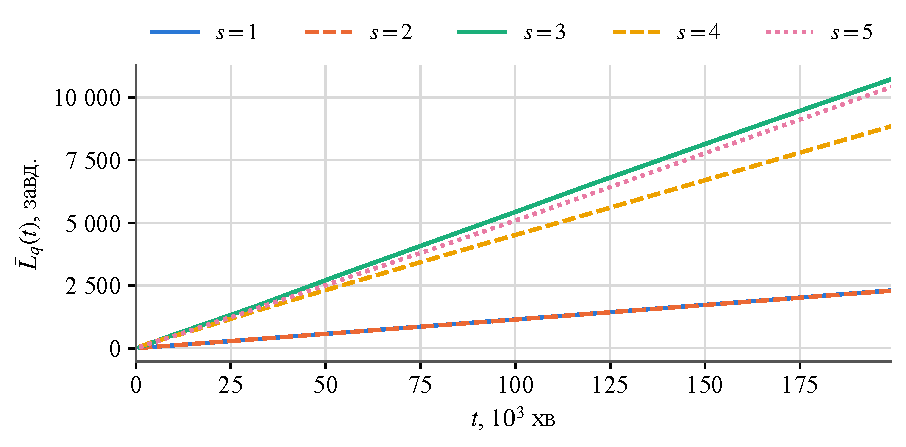
\includegraphics{media/exp-unstable}
  \caption{Середня кількість завдань у черзі на інтервалі $[0;\,t]$ за інтенсивностей з умови
    задачі ($\gamma = 1$, $\lambda_\Sigma = 0{,}33$~завд./хв, середнє за 5~прогонами)}
  \label{fig:exp-unstable}
\end{figure}

Умова $\gamma < 0{,}85$ з формули~\eqref{eq:rho} лише необхідна, тому фактичну межу визначено
прогонами за $\gamma = 0{,}75$ і~0,8 (таблиця~\ref{tab:exp-boundary}). За $\gamma = 0{,}75$ усі
стратегії стійкі: середня черга від часу не залежить, а $U = \rho = 0{,}88$. За $\gamma = 0{,}8$
($\rho = 0{,}94$) черга стратегій 1--2 зростає пропорційно часу, а $U < \rho$: завдання~C з
найнижчим пріоритетом стартує лише тоді, коли вільні обидві одиниці памʼяті й немає завдань A
і~B, а поки воно чекає, вивільнена одиниця простоює, і ці втрати перевищують запас
$1 - \rho = 0{,}06$. У стратегіях 3--5 простій обмежено резервуванням (4~\% памʼяті), і черга
стабілізується.

% Згенеровано experiments/analysis.py — не редагувати вручну
\begin{kpitable}{|c|r|r|r|r|r|r|r|}{Середня кількість завдань у черзі $\bar L_q$ на інтервалі $[0;\,t]$, завд., (5~прогонів, $t$ -- у хв) і коефіцієнт використання памʼяті $U$ (10~прогонів, $T_{\text{мод}} = 3{,}5\cdot10^6$~хв, $T_{\text{п}} = 2\cdot10^4$~хв) за рівнів $\gamma$ понад план експерименту\label{tab:exp-boundary}}
  { & \multicolumn{3}{c|}{\textbf{$\gamma = 0{,}75$ ($\lambda_\Sigma = 0{,}2475$~завд./хв)}} & \multicolumn{4}{c|}{\textbf{$\gamma = 0{,}80$ ($\lambda_\Sigma = 0{,}264$~завд./хв)}} \\ \cline{2-8}
  \textbf{$s$} & \textbf{$t = 2\cdot10^6$} & \textbf{$t = 8\cdot10^6$} & \textbf{$U$} & \textbf{$t = 2\cdot10^6$} & \textbf{$t = 4\cdot10^6$} & \textbf{$t = 8\cdot10^6$} & \textbf{$U$}}
  1 & 11,8 & 11,6 & 0,881 & 796,5 & 1\,721,8 & 3\,675,4 & 0,930 \\ \hline
  2 & 11,5 & 11,3 & 0,882 & 989,9 & 1\,701,6 & 3\,125,5 & 0,932 \\ \hline
  3 & 27,7 & 28,5 & 0,882 & 156,0 & 139,5 & 137,0 & 0,940 \\ \hline
  4 & 25,0 & 24,6 & 0,880 & 111,1 & 103,1 & 106,4 & 0,940 \\ \hline
  5 & 28,3 & 29,4 & 0,882 & 153,3 & 151,1 & 147,8 & 0,940 \\ \hline
\end{kpitable}


План обмежено рівнем $\gamma = 0{,}7$ ($\rho = 0{,}82$), щоб усі стратегії досліджувати на всіх
рівнях за однакових умов: за $\gamma = 0{,}8$ відгуки стратегій 1--2 не стабілізуються, а за
$\gamma = 0{,}75$ для стратегії~1 критерій збіжності (підрозділ~\ref{sec:exp-warmup}) вимагає
$6{,}2\cdot10^6$~хв -- майже вдвічі більше за прийнятий час моделювання. За нижньої межі
$\gamma = 0{,}4$ ($\rho = 0{,}47$) черги майже не утворюються. Метод дослідження обрано за
характером фактора~\cite{stetsenko-kursova}: вплив якісного фактора~$s$ перевірено дисперсійним
аналізом, а залежність відгуків від кількісного фактора~$\gamma$ описано рівняннями регресії.
Дані для обох методів дає повний план $5 \times 7$ з повторними прогонами.

Серії прогонів виконує клас \texttt{ExperimentRunner} із
записом результатів у файли CSV. Seed кожного прогону обчислюється за номером серії, точки плану
й прогону, тож прогони незалежні (і виконуються паралельно), а повторний запуск дає ті самі
результати:
\codeinput[firstline=232, lastline=234, gobble=4]{../sim/src/main/java/ua/kpi/km/b14/experiment/ExperimentRunner.java}
Статистичну обробку і таблиці розділу з файлів CSV виконує скрипт \texttt{analysis.py}
(SciPy~\cite{scipy}); лістинги -- у додатку~В.

\subsection{Перехідний період і час моделювання}\label{sec:exp-warmup}

Імітація починається з порожньої системи, тож відгуки на початку прогону занижені; їх
виключено зі статистики, яку збирають від моменту $T_{\text{п}}$ (таблиця~\ref{tab:kernel-mods}).
Тривалість перехідного періоду визначено за поточною довжиною черги $L_q^*(t)$, усередненою за
ансамблем із 50~прогонів у найбільш навантаженій точці $\gamma = 0{,}7$
(рисунок~\ref{fig:exp-warmup}, ковзне середнє за 2000~хв): вона виходить на сталий рівень за
$(2\ldots5)\cdot10^3$~хв. Оскільки помилка в більший бік не погіршує точності~\cite{stetsenko-kursova},
прийнято $T_{\text{п}} = 2\cdot10^4$~хв -- щонайменше з чотирикратним запасом, що становить лише 0,6~\% $T_{\text{мод}}$.

\begin{figure}
  \centering
  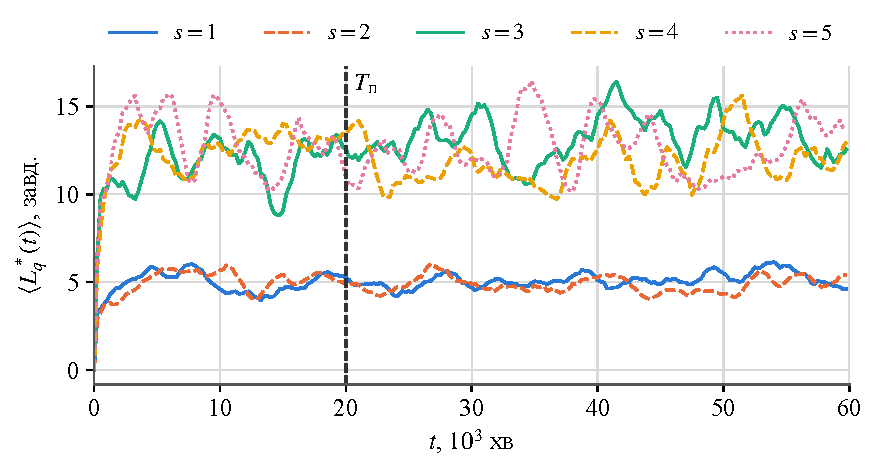
\includegraphics{media/exp-warmup}
  \caption{Поточна кількість завдань у черзі, усереднена за 50~прогонами ($\gamma = 0{,}7$)}
  \label{fig:exp-warmup}
\end{figure}

Час моделювання визначено за критерієм посібника~\cite{stetsenko-kursova}: це момент~$T$, після
якого середні значення відгуку на $[0;\,t]$, обчислені за формулою~\eqref{eq:time-means}, у пробних прогонах
відрізняються менше ніж на задану точність:
\begin{equation}\label{eq:criterion}
  T:\ \forall t \ge T,\ \forall i, j\quad \left|\bar y_i(t) - \bar y_j(t)\right| < \varepsilon,
\end{equation}
де $\bar y_i(t)$ -- середнє відгуку в $i$-му прогоні на $[0;\,t]$, $\varepsilon = 0{,}1\bar y$ --
задана точність (10~\% сталого значення).

Для кожної стратегії за $\gamma = 0{,}4$ і~0,7 виконано по 5~прогонів тривалістю
$5\cdot10^6$~хв (середні записано кожні $2{,}5\cdot10^4$~хв); значення~$T$ наведено в
таблиці~\ref{tab:exp-criterion}, приклад траєкторій -- на рисунку~\ref{fig:exp-criterion}: середні
окремих прогонів сходяться до одного рівня, тобто відгуки з часом стабілізуються. Що більше
навантаження, то довше відгуки збігаються (за $\gamma = 0{,}4$ достатньо $T \le 5{,}5\cdot10^5$~хв, за
$\gamma = 0{,}7$ потрібно до $3{,}3\cdot10^6$~хв), бо довгі черги повільно «забувають» свій стан;
найповільніше збігається~$L_q$, а $W$ містить сталу складову (час виконання) і збігається швидше. Для всіх точок плану прийнято $T_{\text{мод}} = 3{,}5\cdot10^6$~хв, що задовольняє
критерій~\eqref{eq:criterion} і в найгіршій точці ($T = 3{,}3\cdot10^6$~хв); статистику збирають на інтервалі
$[2\cdot10^4;\,3{,}5\cdot10^6]$~хв. Такий прогін за $\gamma = 0{,}7$ (близько
$8\cdot10^5$ надходжень) триває менше секунди.

% Згенеровано experiments/analysis.py — не редагувати вручну
\begin{kpitable}{|c|r|r|r|r|r|r|}{Найменший час моделювання за критерієм~\eqref{eq:criterion} ($\varepsilon = 10$~\% сталого значення, 5 прогонів), $10^6$~хв\label{tab:exp-criterion}}
  { & \multicolumn{3}{c|}{\textbf{$\gamma = 0{,}4$}} & \multicolumn{3}{c|}{\textbf{$\gamma = 0{,}7$}} \\ \cline{2-7}
  \textbf{$s$} & \textbf{$W$} & \textbf{$L_q$} & \textbf{$W_q$} & \textbf{$W$} & \textbf{$L_q$} & \textbf{$W_q$}}
  1 & 0,05 & 0,55 & 0,55 & 1,62 & 3,30 & 3,27 \\ \hline
  2 & 0,03 & 0,23 & 0,07 & 1,98 & 2,85 & 2,60 \\ \hline
  3 & 0,15 & 0,53 & 0,53 & 0,90 & 1,10 & 1,07 \\ \hline
  4 & 0,28 & 0,35 & 0,35 & 0,78 & 3,20 & 1,07 \\ \hline
  5 & 0,12 & 0,17 & 0,17 & 2,65 & 2,80 & 2,80 \\ \hline
\end{kpitable}


\begin{figure}
  \centering
  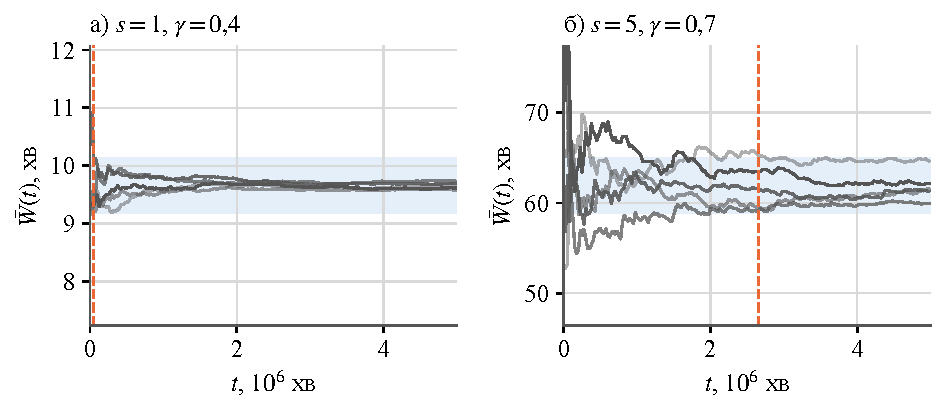
\includegraphics{media/exp-criterion}
  \caption{Середній час перебування на інтервалі $[0;\,t]$ у пʼяти прогонах ($T_{\text{п}} = 0$;
    смуга -- $\bar y \pm \varepsilon/2$, $\varepsilon = 10$~\%; штрихова лінія -- момент~$T$
    за критерієм~\eqref{eq:criterion})}
  \label{fig:exp-criterion}
\end{figure}

\subsection{Кількість прогонів і точність результатів}\label{sec:exp-runs}

Результат експерименту -- середнє відгуку за $p$ незалежними прогонами. Розкид оцінено
серією по 100~прогонів кожної стратегії за $\gamma = 0{,}7$, де він найбільший.
Центральну граничну теорему для визначення~$p$ можна застосувати лише за розподілу відгуку,
близького до нормального~\cite{stetsenko-kursova}; нормальність перевірено за критерієм згоди $\chi^2$~\cite{stetsenko-modeling} (10~рівноймовірних
інтервалів, 7~ступенів вільності, $\chi^2_{\text{кр}} = 14{,}07$ за рівня значущості 0,05).

Для стратегій 2--5 гіпотезу про нормальний закон не відхилено ($\chi^2 = 1{,}8\ldots14{,}0$), а
для стратегії~1 відхилено за всіма трьома відгуками ($\chi^2 = 14{,}8\ldots16{,}6$,
таблиця~\ref{tab:exp-pilot}; гістограма на рисунку~\ref{fig:exp-hist},~а несиметрична й має
кілька вершин). Отже, нормальність відгуку гарантувати не можна, і кількість прогонів визначено
за наслідком нерівності Чебишова~\cite{stetsenko-kursova}:
\begin{equation}\label{eq:chebyshev}
  p = \frac{\sigma^2}{\varepsilon^2\,(1-\beta)},
\end{equation}
де $\sigma$ -- стандартне відхилення відгуку в серії, $\varepsilon = 0{,}02\bar y$ --
задана точність результату (2~\% середнього), $\beta = 0{,}95$ -- довірча ймовірність.

\begin{figure}
  \centering
  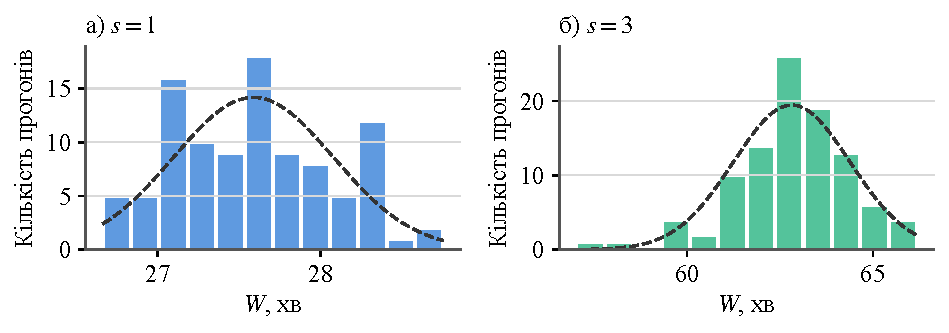
\includegraphics{media/exp-hist}
  \caption{Гістограми середнього часу перебування за 100~прогонами ($\gamma = 0{,}7$,
    $T_{\text{мод}} = 3{,}5\cdot10^6$~хв, $T_{\text{п}} = 2\cdot10^4$~хв); штрихова лінія --
    нормальний закон з вибірковими параметрами}
  \label{fig:exp-hist}
\end{figure}

% Згенеровано experiments/analysis.py — не редагувати вручну
\begin{kpitable}{|c|r|r|r|r|r|r|r|r|r|}{Розкид відгуків, критерій $\chi^2$ і потрібна кількість прогонів ($\gamma = 0{,}7$, 100 прогонів, $T_{\text{мод}} = 3{,}5\cdot10^6$~хв, $T_{\text{п}} = 2\cdot10^4$~хв, $\varepsilon = 2$~\% середнього, $\beta = 0{,}95$, $\chi^2_{\text{кр}} = 14{,}07$)\label{tab:exp-pilot}}
  { & \multicolumn{3}{c|}{\textbf{$\sigma/\bar y$, \%}} & \multicolumn{3}{c|}{\textbf{$\chi^2$}} & \multicolumn{3}{c|}{\textbf{$p$ за~\eqref{eq:chebyshev}}} \\ \cline{2-10}
  \textbf{$s$} & \textbf{$W$} & \textbf{$L_q$} & \textbf{$W_q$} & \textbf{$W$} & \textbf{$L_q$} & \textbf{$W_q$} & \textbf{$W$} & \textbf{$L_q$} & \textbf{$W_q$}}
  1 & 1,8 & 2,2 & 2,2 & 16,6 & 16,4 & 14,8 & 16 & 25 & 24 \\ \hline
  2 & 1,8 & 2,2 & 2,2 & 9,8 & 10,6 & 14,0 & 16 & 25 & 24 \\ \hline
  3 & 2,5 & 2,8 & 2,7 & 6,2 & 5,0 & 5,8 & 32 & 39 & 37 \\ \hline
  4 & 2,2 & 2,5 & 2,5 & 7,8 & 6,4 & 6,6 & 26 & 32 & 31 \\ \hline
  5 & 2,9 & 3,2 & 3,2 & 2,6 & 3,8 & 1,8 & 43 & 52 & 50 \\ \hline
\end{kpitable}


Найбільшу кількість прогонів -- 52 -- потребує $L_q$ для стратегії~5 (за центральною граничною
теоремою було б не більше 10), тому прийнято $p = 60$ прогонів у кожній точці плану. За менших
$\gamma$ розкид менший: за результатами факторного експерименту стандартне відхилення відгуку між
прогонами становить 0,4--2,8~\% середнього, точність, гарантована
нерівністю Чебишова для 60~прогонів, $\varepsilon = \sigma/\sqrt{p(1-\beta)}$, не гірша за 1,63~\%
середнього в усіх 35~точках, а половина довірчого інтервалу за розподілом Стьюдента -- не
більша за 0,73~\%.

Точності $\varepsilon = 10$~\% у критерії~\eqref{eq:criterion} і 2~\% у
формулі~\eqref{eq:chebyshev} мають різне призначення: перша визначає тривалість прогону, за якої
його середнє перестає залежати від часу, друга -- точність результату, яку забезпечує
усереднення $p$ прогонів. За $T_{\text{мод}}$ розмах середніх пʼяти прогонів становить до 9,5~\%
($L_q$, $s = 1$, $\gamma = 0{,}7$), стандартне відхилення між прогонами серії --
1,8--3,2~\% середнього, а усереднення 60~прогонів зменшує його в $\sqrt{60} \approx 7{,}7$~раза.
З $\varepsilon = 2$~\% критерій~\eqref{eq:criterion} не виконується в межах
$5\cdot10^6$~хв у 23 з 30~випадків, і одному прогону знадобилося б близько $8\cdot10^7$~хв
(розмах середніх спадає як $1/\sqrt{t}$), тоді як 60~прогонів охоплюють у точці
$2{,}1\cdot10^8$~хв модельного часу.

\subsection{Результати факторного експерименту}\label{sec:exp-results}

Повний факторний план $5 \times 7$ за $p = 60$ містить 2100~прогонів ($1{,}3\cdot10^9$
завдань, що пройшли через систему) і виконується близько 40~с. Залежність $W$
від~$\gamma$ наведено на рисунку~\ref{fig:exp-w} (точки -- експеримент,
лінії -- рівняння регресії з підрозділу~\ref{sec:exp-regression}; довірчі інтервали менші за
маркери), залежність $L_q$ -- на рисунку~\ref{fig:exp-lq}, а $W_q$ має той самий вигляд, що й~$W$; показники за типами завдань наведено в
таблиці~\ref{tab:exp-bytype} додатка~В.

\begin{figure}
  \centering
  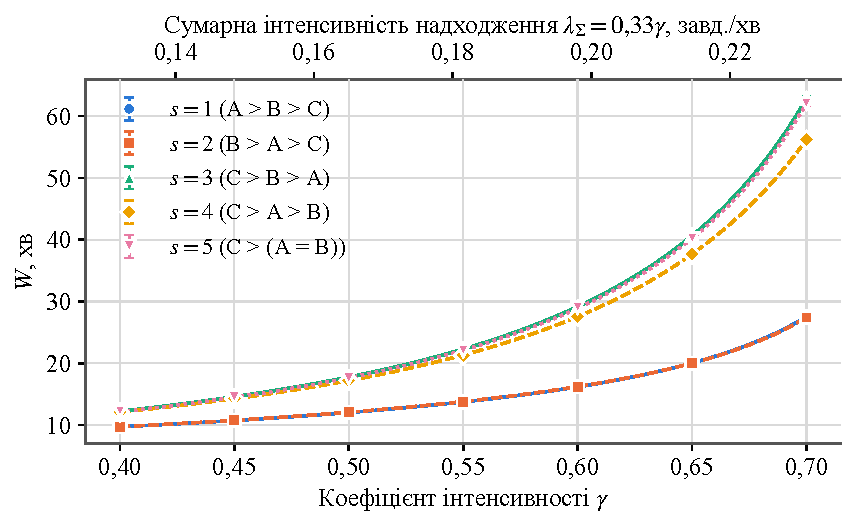
\includegraphics{media/exp-w}
  \caption{Залежність середнього часу перебування в системі від коефіцієнта інтенсивності
    ($T_{\text{мод}} = 3{,}5\cdot10^6$~хв, $T_{\text{п}} = 2\cdot10^4$~хв, 60~прогонів)}
  \label{fig:exp-w}
\end{figure}

Стратегії утворюють дві чітко розділені групи. Стратегії 1 і~2, у яких завдання~C мають
найнижчий пріоритет, дають найменші значення всіх трьох відгуків, і перевага зростає з
навантаженням: $W$ менший на 20--21~\% за $\gamma = 0{,}4$ і у 2,0--2,3 раза за $\gamma = 0{,}7$.
Короткі завдання A і~B (82~\% потоку) тут не чекають довгих завдань~C, а у стратегіях 3--5
кожне завдання~C блокує старт A і~B до звільнення всієї памʼяті (за $\gamma = 0{,}7$ через
резервування простоює 3,5~\% памʼяті). Усередині груп відмінності значно менші: стратегії 1 і~2 практично однакові, бо часи
виконання A і~B близькі, а серед 3--5 найкраща стратегія~4 (C~$>$~A~$>$~B), у якій вищий
пріоритет має найчисельніший потік коротких завдань~A. Ціна виграшу -- перерозподіл очікування
між типами: за $\gamma = 0{,}7$ завдання~C у стратегіях 1--2 перебувають у системі 99--101~хв
проти 22~хв у стратегіях 3--5, у стратегії~4 так само страждають завдання~B ($W_B = 137$~хв), а у
стратегії~3 -- завдання~A ($W_A = 88$~хв).

\begin{figure}
  \centering
  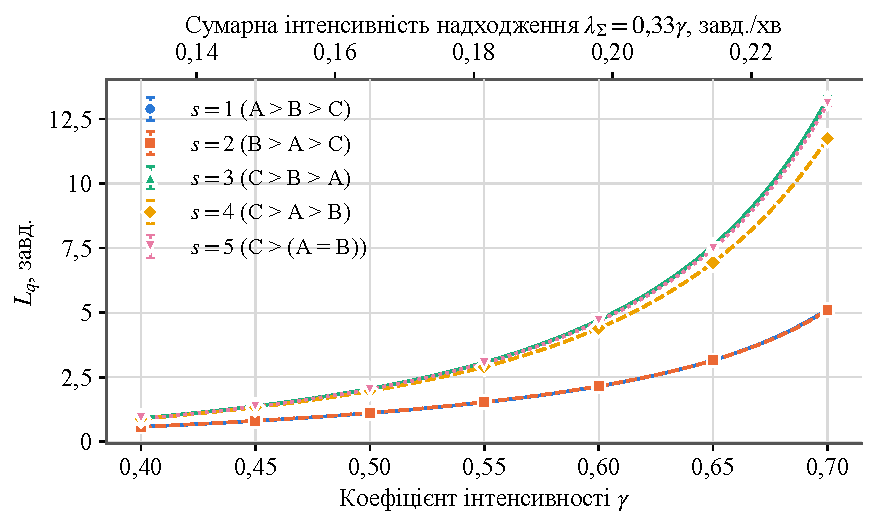
\includegraphics{media/exp-lq}
  \caption{Залежність середньої кількості завдань у черзі від коефіцієнта інтенсивності
    ($T_{\text{мод}} = 3{,}5\cdot10^6$~хв, $T_{\text{п}} = 2\cdot10^4$~хв, 60~прогонів)}
  \label{fig:exp-lq}
\end{figure}

Середні значення $W$ і $L_q$ та половини довірчих інтервалів наведено в
таблицях~\ref{tab:exp-w} і~\ref{tab:exp-lq}.

% Згенеровано experiments/analysis.py — не редагувати вручну
\begingroup\setlength{\tabcolsep}{2.5pt}
\begin{kpitable}{|c|c|r|r|r|r|r|}{Середнє значення $W$, хв, і половина довірчого інтервалу ($\beta = 0{,}95$, 60 прогонів, $T_{\text{мод}} = 3{,}5\cdot10^6$~хв, $T_{\text{п}} = 2\cdot10^4$~хв)\label{tab:exp-w}}
  {\textbf{$\gamma$} & \textbf{\begin{tabular}{@{}c@{}}$\lambda_\Sigma$,\\ завд./хв\end{tabular}} & \textbf{$s = 1$} & \textbf{$s = 2$} & \textbf{$s = 3$} & \textbf{$s = 4$} & \textbf{$s = 5$}}
  0,40 & 0,132 & 9,71$\pm$0,01 & 9,73$\pm$0,01 & 12,26$\pm$0,02 & 12,09$\pm$0,03 & 12,20$\pm$0,02 \\ \hline
  0,45 & 0,1485 & 10,73$\pm$0,02 & 10,76$\pm$0,01 & 14,56$\pm$0,03 & 14,27$\pm$0,03 & 14,48$\pm$0,04 \\ \hline
  0,50 & 0,165 & 12,02$\pm$0,02 & 12,07$\pm$0,02 & 17,75$\pm$0,05 & 17,20$\pm$0,05 & 17,57$\pm$0,05 \\ \hline
  0,55 & 0,1815 & 13,73$\pm$0,02 & 13,79$\pm$0,03 & 22,26$\pm$0,07 & 21,30$\pm$0,06 & 22,04$\pm$0,06 \\ \hline
  0,60 & 0,198 & 16,18$\pm$0,04 & 16,22$\pm$0,04 & 29,08$\pm$0,12 & 27,55$\pm$0,11 & 29,00$\pm$0,11 \\ \hline
  0,65 & 0,2145 & 20,02$\pm$0,06 & 20,01$\pm$0,06 & 40,72$\pm$0,23 & 37,67$\pm$0,16 & 40,17$\pm$0,19 \\ \hline
  0,70 & 0,231 & 27,53$\pm$0,14 & 27,40$\pm$0,13 & 62,82$\pm$0,41 & 56,20$\pm$0,28 & 62,04$\pm$0,40 \\ \hline
\end{kpitable}
\endgroup

% Згенеровано experiments/analysis.py — не редагувати вручну
\begingroup\setlength{\tabcolsep}{2.5pt}
\begin{kpitable}{|c|c|r|r|r|r|r|}{Середнє значення $L_q$, завд., і половина довірчого інтервалу ($\beta = 0{,}95$, 60 прогонів, $T_{\text{мод}} = 3{,}5\cdot10^6$~хв, $T_{\text{п}} = 2\cdot10^4$~хв)\label{tab:exp-lq}}
  {\textbf{$\gamma$} & \textbf{\begin{tabular}{@{}c@{}}$\lambda_\Sigma$,\\ завд./хв\end{tabular}} & \textbf{$s = 1$} & \textbf{$s = 2$} & \textbf{$s = 3$} & \textbf{$s = 4$} & \textbf{$s = 5$}}
  0,40 & 0,132 & 0,582$\pm$0,001 & 0,584$\pm$0,002 & 0,917$\pm$0,003 & 0,895$\pm$0,003 & 0,910$\pm$0,003 \\ \hline
  0,45 & 0,1485 & 0,806$\pm$0,003 & 0,811$\pm$0,002 & 1,374$\pm$0,005 & 1,332$\pm$0,005 & 1,362$\pm$0,005 \\ \hline
  0,50 & 0,165 & 1,109$\pm$0,003 & 1,118$\pm$0,003 & 2,053$\pm$0,008 & 1,964$\pm$0,008 & 2,025$\pm$0,008 \\ \hline
  0,55 & 0,1815 & 1,529$\pm$0,004 & 1,540$\pm$0,005 & 3,08$\pm$0,01 & 2,90$\pm$0,01 & 3,04$\pm$0,01 \\ \hline
  0,60 & 0,198 & 2,153$\pm$0,007 & 2,162$\pm$0,007 & 4,71$\pm$0,02 & 4,41$\pm$0,02 & 4,69$\pm$0,02 \\ \hline
  0,65 & 0,2145 & 3,16$\pm$0,01 & 3,15$\pm$0,01 & 7,60$\pm$0,05 & 6,94$\pm$0,03 & 7,48$\pm$0,04 \\ \hline
  0,70 & 0,231 & 5,14$\pm$0,03 & 5,11$\pm$0,03 & 13,29$\pm$0,10 & 11,75$\pm$0,06 & 13,10$\pm$0,09 \\ \hline
\end{kpitable}
\endgroup


Значення $W_q$ наведено в таблиці~\ref{tab:exp-wq}.

% Згенеровано experiments/analysis.py — не редагувати вручну
\begingroup\setlength{\tabcolsep}{2.5pt}
\begin{kpitable}{|c|c|r|r|r|r|r|}{Середнє значення $W_q$, хв, і половина довірчого інтервалу ($\beta = 0{,}95$, 60 прогонів, $T_{\text{мод}} = 3{,}5\cdot10^6$~хв, $T_{\text{п}} = 2\cdot10^4$~хв)\label{tab:exp-wq}}
  {\textbf{$\gamma$} & \textbf{\begin{tabular}{@{}c@{}}$\lambda_\Sigma$,\\ завд./хв\end{tabular}} & \textbf{$s = 1$} & \textbf{$s = 2$} & \textbf{$s = 3$} & \textbf{$s = 4$} & \textbf{$s = 5$}}
  0,40 & 0,132 & 4,41$\pm$0,01 & 4,42$\pm$0,01 & 6,95$\pm$0,02 & 6,78$\pm$0,02 & 6,90$\pm$0,02 \\ \hline
  0,45 & 0,1485 & 5,43$\pm$0,02 & 5,46$\pm$0,01 & 9,25$\pm$0,03 & 8,97$\pm$0,03 & 9,17$\pm$0,03 \\ \hline
  0,50 & 0,165 & 6,72$\pm$0,02 & 6,77$\pm$0,02 & 12,44$\pm$0,05 & 11,90$\pm$0,05 & 12,27$\pm$0,05 \\ \hline
  0,55 & 0,1815 & 8,42$\pm$0,02 & 8,48$\pm$0,03 & 16,96$\pm$0,07 & 16,00$\pm$0,06 & 16,74$\pm$0,06 \\ \hline
  0,60 & 0,198 & 10,87$\pm$0,04 & 10,92$\pm$0,04 & 23,78$\pm$0,12 & 22,25$\pm$0,10 & 23,70$\pm$0,11 \\ \hline
  0,65 & 0,2145 & 14,72$\pm$0,06 & 14,70$\pm$0,06 & 35,42$\pm$0,23 & 32,36$\pm$0,16 & 34,87$\pm$0,19 \\ \hline
  0,70 & 0,231 & 22,23$\pm$0,14 & 22,10$\pm$0,13 & 57,52$\pm$0,41 & 50,90$\pm$0,28 & 56,73$\pm$0,40 \\ \hline
\end{kpitable}
\endgroup


Вплив складу потоку перевірено серією, у якій змінюється лише потік завдань~C:
$\lambda_C = \gamma_C\cdot0{,}6\lambda_C^0$, $\gamma_C \in \{0{,}5;\,1;\,1{,}25\}$ за $\lambda_A$
і~$\lambda_B$ рівня $\gamma = 0{,}6$, для найкращих стратегій обох груп -- 1 і~4
(таблиця~\ref{tab:exp-flows}). За $\gamma_C = 1{,}25$ навантаження $\rho = 0{,}795$ не більше,
ніж у плані, тож $T_{\text{п}}$, $T_{\text{мод}}$ і $p = 60$ ті самі (точність не гірша за 1,30~\%);
точка $\gamma_C = 1$ збігається з точкою плану $\gamma = 0{,}6$ (різниця $W$ -- до 0,25~\%).

% Згенеровано experiments/analysis.py — не редагувати вручну
\begin{kpitable}{|c|c|c|c|r|r|r|r|}{Відгуки за зміни лише потоку завдань~C ($\lambda_A = 0{,}12$, $\lambda_B = 0{,}042$~завд./хв, 60~прогонів, $T_{\text{мод}} = 3{,}5\cdot10^6$~хв, $T_{\text{п}} = 2\cdot10^4$~хв)\label{tab:exp-flows}}
  {\textbf{$\gamma_C$} & \textbf{$\lambda_C$, завд./хв} & \textbf{$\rho$} & \textbf{$s$} & \textbf{$W$, хв} & \textbf{$L_q$, завд.} & \textbf{$W_q$, хв} & \textbf{$W_C$, хв}}
  0,5 & 0,018 & 0,525 & 1 & 8,81 & 0,72 & 3,97 & 22,69 \\ \hline
  0,5 & 0,018 & 0,525 & 4 & 11,14 & 1,14 & 6,31 & 15,28 \\ \hline
  1,0 & 0,036 & 0,705 & 1 & 16,16 & 2,15 & 10,86 & 45,18 \\ \hline
  1,0 & 0,036 & 0,705 & 4 & 27,62 & 4,42 & 22,32 & 19,46 \\ \hline
  1,25 & 0,045 & 0,795 & 1 & 25,96 & 4,23 & 20,45 & 80,08 \\ \hline
  1,25 & 0,045 & 0,795 & 4 & 50,45 & 9,30 & 44,94 & 22,57 \\ \hline
\end{kpitable}


Стратегія~1 лишається кращою за всіма відгуками за кожного~$\gamma_C$ ($W$ у стратегії~4 більший
у 1,26--1,94~раза), тож найкраща стратегія від співвідношення потоків не залежить. Проте
перерозподіл очікування посилюється: у стратегії~1 $W_C$ зростає в 3,5~раза, а у стратегії~4
завдання~B за $\gamma_C = 1{,}25$ перебувають у системі 112~хв.

\subsection{Дисперсійний аналіз впливу стратегії упорядкування}\label{sec:exp-anova}

Дисперсійний аналіз і перевірка рівнянь регресії припускають однаковий розкид відгуку між
прогонами в усіх точках плану, тобто відтворюваність експерименту. Її перевірено за критерієм
Кохрена~\cite{stetsenko-modeling}:
\begin{equation}\label{eq:cochran}
  G = \frac{\max_j s_j^2}{\sum_{j=1}^{N} s_j^2}, \qquad
  s_j^2 = \frac{1}{p-1}\sum_{k=1}^{p}\left(y_{jk} - \bar y_j\right)^2,
\end{equation}
де $y_{jk}$ і $\bar y_j$ -- відгук у $k$-му прогоні й середнє $j$-ї точки плану, $N = 35$ --
кількість точок. Дисперсії однорідні, якщо $G < G_{\text{кр}}$ (таблиця~\ref{tab:exp-cochran}); для $\alpha = 0{,}05$, $N = 35$ і
$p - 1 = 59$ ступенів вільності $G_{\text{кр}} = 0{,}046$.

% Згенеровано experiments/analysis.py — не редагувати вручну
\begingroup\setlength{\tabcolsep}{2pt}
\begin{kpitable}{|c|c|c|c|c|c|}{Перевірка відтворюваності за критерієм Кохрена ($\alpha = 0{,}05$; повний план -- 35~точок по 60~прогонів)\label{tab:exp-cochran}}
  {\textbf{Відгук} & \textbf{Повний план} & \textbf{$\gamma \in \{0{,}40;\,0{,}45\}$} & \textbf{$\gamma \in \{0{,}65;\,0{,}70\}$} & \textbf{Один рівень $\gamma$} & \textbf{$p = 20$}}
  $W$ & 0,271 & 0,211 & 0,304 & 0,310--0,427 & 0,305 \\ \hline
  $L_q$ & 0,294 & 0,231 & 0,318 & 0,301--0,426 & 0,326 \\ \hline
  $W_q$ & 0,273 & 0,216 & 0,305 & 0,313--0,428 & 0,308 \\ \hline
  $G_{\text{кр}}$ & 0,046 & 0,150 & 0,150 & 0,282 & 0,063 \\ \hline
\end{kpitable}
\endgroup


Для всіх відгуків $G$ у 6~разів більший за критичне значення:
дисперсії неоднорідні, найбільша з них -- у точці $s = 3$, $\gamma = 0{,}7$, а відношення
найбільшої дисперсії до найменшої сягає 1395--5428. Рекомендовані для невідтворюваного
експерименту засоби~\cite{stetsenko-modeling} -- звуження інтервалу варіювання і збільшення
кількості прогонів -- однорідності не дають: $G > G_{\text{кр}}$ і для двох сусідніх рівнів~$\gamma$,
і для кожного рівня окремо, де дисперсії пʼяти стратегій різняться в 5--15~разів, а за
$p = 10$, 20, 40, 60 критерій $G$ спадає від 0,41--0,44 лише до 0,27--0,29 (при $G_{\text{кр}}$ від
0,083 до 0,046). Отже, розкид залежить і від навантаження, і від стратегії; неоднорідність є
властивістю системи й без відмови від мети моделювання не усувається, тому далі показано, що
висновки дисперсійного аналізу від неї не залежать.

Різниця між стратегіями зростає з навантаженням (рисунки~\ref{fig:exp-w} і~\ref{fig:exp-lq}),
тому вплив стратегії перевірено однофакторним дисперсійним аналізом~\cite{stetsenko-kursova}
окремо на кожному рівні~$\gamma$. Для рівня з $q = 5$ стратегіями і $p = 60$ прогонами кожної
факторна і залишкова дисперсії
\begin{equation}\label{eq:anova-ss}
  D_F = \frac{p}{q-1}\sum_{a=1}^{q}\left(\bar y_a - \bar y\right)^2, \qquad
  D_R = \frac{1}{q(p-1)}\sum_{a=1}^{q}\sum_{k=1}^{p}\left(y_{ak} - \bar y_a\right)^2,
\end{equation}
де $y_{ak}$ -- відгук у $k$-му прогоні за стратегії~$a$, $\bar y_a$ -- середнє за стратегією,
$\bar y$ -- загальне середнє рівня. Вплив стратегії значущий, якщо відношення дисперсій~\eqref{eq:anova-ss} $F = D_F/D_R > F_{\text{кр}}$ --
квантиля розподілу Фішера рівня $1-\alpha$ зі ступенями вільності $q-1$ і $q(p-1)$,
$\alpha = 0{,}05$; результати наведено в таблиці~\ref{tab:exp-anova1}.

% Згенеровано experiments/analysis.py — не редагувати вручну
\begin{kpitable}{|c|r|r|r|c|}{Значення критерію Фішера для впливу стратегії на кожному рівні $\gamma$ ($\alpha = 0{,}05$)\label{tab:exp-anova1}}
  {\textbf{$\gamma$} & \textbf{$F$ для $W$} & \textbf{$F$ для $L_q$} & \textbf{$F$ для $W_q$} & \textbf{$F_{\text{кр}}$}}
  0,40 & 17\,215,7 & 18\,463,8 & 19\,858,6 & 2,40 \\ \hline
  0,45 & 22\,081,0 & 22\,912,8 & 24\,450,2 & 2,40 \\ \hline
  0,50 & 21\,678,4 & 21\,829,3 & 23\,052,1 & 2,40 \\ \hline
  0,55 & 29\,747,1 & 29\,559,0 & 31\,116,8 & 2,40 \\ \hline
  0,60 & 23\,047,8 & 22\,848,9 & 23\,638,6 & 2,40 \\ \hline
  0,65 & 19\,216,5 & 18\,915,3 & 19\,461,2 & 2,40 \\ \hline
  0,70 & 15\,031,4 & 14\,791,5 & 15\,130,2 & 2,40 \\ \hline
\end{kpitable}


На всіх семи рівнях і для всіх відгуків $F \ge 14\,791$ при $F_{\text{кр}} = 2{,}40$, тобто
стратегія впливає на всі три відгуки за будь-якої інтенсивності з досліджуваного діапазону.
Вплив кількісного фактора~$\gamma$ оцінено регресійним аналізом
(підрозділ~\ref{sec:exp-regression}).

Висновки стійкі до неоднорідності дисперсій: у межах одного рівня~$\gamma$ дисперсії пʼяти
стратегій різняться лише в 5--15~разів (проти 1395--5428 у плані загалом), кількість прогонів
для всіх стратегій однакова, а $F$ перевищує критичне значення понад у 6000~разів.

Значущість впливу фактора ще не означає, що різні всі його рівні, тому близькі стратегії
порівняно попарно однофакторним аналізом із двома рівнями за~$W$
($F_{\text{кр}} = 3{,}92$). Різниці між стратегіями 1 і~2 (до 0,47~\%,
на чотирьох рівнях~$\gamma$ незначуща) і між 3 і~5 (до 1,35~\%, хоча значуща на шести рівнях)
менші за задану точність 2~\%, тож ці пари практично рівноцінні. Перевага стратегії~4 над 5 і~3 значуща на
всіх рівнях ($F \ge 40{,}1$) і зростає від 0,9--1,4~\% за $\gamma = 0{,}4$ до 10,4--11,8~\% за
$\gamma = 0{,}7$.

\subsection{Регресійний аналіз залежності відгуків від інтенсивності}\label{sec:exp-regression}

Залежність відгуків від~$\gamma$ описано рівняннями регресії, лінійними за
параметрами~\cite{stetsenko-kursova}. Черга зростає пропорційно $1/(1-\rho)$, а для завдань
нижчого пріоритету -- ще швидше, тому функцією фактора обрано
$z = 1/(1 - \gamma\rho^0)$, $z \in [1{,}89;\,5{,}63]$, і за рекомендацією
посібника~\cite{stetsenko-kursova} нормалізовано її до інтервалу $[-1;\,1]$:
\begin{equation}\label{eq:normalization}
  x = \frac{z - z_0}{\Delta z}, \qquad z_0 = \frac{z_{\max} + z_{\min}}{2} = 3{,}760, \qquad
  \Delta z = \frac{z_{\max} - z_{\min}}{2} = 1{,}874.
\end{equation}
Повною моделлю прийнято поліном третього степеня від~$x$ за формулою~\eqref{eq:normalization}:
\begin{equation}\label{eq:regression}
  y = b_0 + b_1 x + b_2 x^2 + b_3 x^3.
\end{equation}
Коефіцієнти знайдено методом найменших квадратів $b = (X^{\mathrm T}X)^{-1}X^{\mathrm T}Y$ за
сімома середніми $\bar y_j$ кожної стратегії і перевірено за процедурою регресійного
аналізу~\cite{stetsenko-modeling}. Коефіцієнт $b_i$ значущий за критерієм Стьюдента, якщо
\begin{equation}\label{eq:student}
  t_i = \frac{|b_i|}{s_{b_i}} > t_{\text{кр}}, \qquad
  s_{b_i}^2 = \frac{c_{ii}\,s^2_{\text{відтв}}}{p}, \qquad
  s^2_{\text{відтв}} = \frac{1}{N}\sum_{j=1}^{N} s_j^2,
\end{equation}
де $c_{ii}$ -- діагональний елемент матриці $(X^{\mathrm T}X)^{-1}$, $s^2_{\text{відтв}}$ --
дисперсія відтворюваності (середня з дисперсій~\eqref{eq:cochran} $N = 7$ точок), $t_{\text{кр}} =
1{,}97$ -- квантиль розподілу Стьюдента рівня $1 - \alpha/2$ для $N(p-1) = 413$ ступенів вільності.
Незначущі доданки відкидають і перераховують коефіцієнти. Рівняння з $d$ коефіцієнтами
адекватне за критерієм Фішера, якщо
\begin{equation}\label{eq:fisher}
  F = \frac{s^2_{\text{ад}}}{s^2_{\text{відтв}}} < F_{\text{кр}}, \qquad
  s^2_{\text{ад}} = \frac{p}{N-d}\sum_{j=1}^{N}\left(\bar y_j - \hat y_j\right)^2,
\end{equation}
де $\hat y_j$ -- значення за рівнянням регресії, $F_{\text{кр}}$ -- квантиль розподілу Фішера
рівня $1-\alpha$ зі ступенями вільності $N - d$ і $N(p-1)$.

За формулою~\eqref{eq:student} коефіцієнти $b_0$, $b_1$, $b_2$ значущі в усіх 15~рівняннях
($t_i \ge 24{,}9$), а $b_3$ незначущий для $W$ і~$W_q$ у стратегіях 3 і~5 ($t_3 = 0{,}5\ldots1{,}1$),
тож для них доданок $x^3$ відкинуто й рівняння квадратичне; в інших 11~рівняннях
$t_3 = 2{,}4\ldots7{,}5$. За формулою~\eqref{eq:fisher} усі 15~отриманих рівнянь адекватні:
$F = 0{,}05\ldots1{,}25$ при $F_{\text{кр}} = 2{,}39$ ($d = 3$) і 2,63 ($d = 4$). Оскільки дисперсії точок неоднорідні, $s^2_{\text{відтв}}$ -- лише середня дисперсія, і висновок
про адекватність наближений; його підтверджує найбільша відносна похибка рівнянь
$\delta_{\max} = \max_j |\bar y_j - \hat y_j|/\bar y_j \le 1{,}23$~\%, менша за точність
експерименту 2~\%, та індекс кореляції
$R = \sqrt{1 - \sum_j (\bar y_j - \hat y_j)^2 / \sum_j (\bar y_j - \bar y)^2} \ge 0{,}99999$ ($\bar y$ -- середнє
з~$\bar y_j$). Коефіцієнти наведено в таблиці~\ref{tab:exp-regression} додатка~В. Простіші
види залежності, перевірені для порівняння, -- квадратичний поліном від~$z$ і поліноми від
самого~$\gamma$ -- для частини рівнянь неадекватні або мають похибку понад 2~\%.

Завдяки нормалізації коефіцієнти порівнянні ($b_0$ -- відгук у центрі діапазону,
$\gamma \approx 0{,}62$), наприклад, $W_{s=1} = 17{,}82 + 8{,}50x + 0{,}80x^2 + 0{,}42x^3$~хв і
$W_{s=4} = 31{,}88 + 22{,}40x + 2{,}27x^2 - 0{,}35x^3$~хв.
Переважає лінійний вплив~$z$ ($b_1$ у 5--12~разів більший за $|b_2|$), а відгуки стратегій
3--5 чутливіші до навантаження: $b_1$ у них у 2,5--3,0, а $b_2$ у 2,8--4,9~раза більші, ніж у 1--2.
Отже, рівняння~\eqref{eq:regression} адекватно описують залежність відгуків від інтенсивності
надходження в діапазоні $\gamma \in [0{,}4;\,0{,}7]$ і можуть замінити імітацію для наближеної
оцінки відгуків усередині цього діапазону.

\subsection{Висновки до розділу}

За інтенсивностей з умови задачі черги зростають необмежено, тому експерименти проведено за
$\gamma \in [0{,}4;\,0{,}7]$ ($T_{\text{п}} = 2\cdot10^4$~хв, $T_{\text{мод}} = 3{,}5\cdot10^6$~хв,
60~прогонів у точці, точність 2~\%); за $\gamma = 0{,}8$ першими втрачають стійкість стратегії 1--2.
Попри неоднорідність дисперсій (критерій Кохрена) дисперсійний аналіз надійно показав значущий
вплив стратегії на всі три відгуки за кожного рівня інтенсивності, причому різниця між
стратегіями зростає з~$\gamma$. Рівноцінні стратегії 1 і~2
(C -- з найнижчим пріоритетом) дають найменші значення відгуків (середній час перебування в
1,25 раза менший за $\gamma = 0{,}4$ і у 2,0--2,3 раза за $\gamma = 0{,}7$, ніж у стратегій 3--5)
коштом завдань~C; серед стратегій із пріоритетом~C найкраща стратегія~4. Зміна лише потоку~C
вибору не змінила. Залежність відгуків від інтенсивності описано адекватними рівняннями регресії
від нормалізованого фактора $1/(1-\rho)$ з похибкою до 1,2~\%.

\section{Інтерпретація результатів моделювання, формулювання висновків та пропозицій}

\subsection{Інтерпретація результатів моделювання}

Верифікована модель (розділ~3) відтворює правила системи за припущення $M = 2$ і в окремих
випадках збігається з аналітичним розвʼязком; фактори -- названі метою моделювання стратегія й
інтенсивність надходження. За потоку з умови памʼяті бракує 17,5~\% і черга зростає необмежено
(рисунок~\ref{fig:exp-unstable}), тому інтенсивності зменшено коефіцієнтом~$\gamma$, а для
заданого потоку потрібна зміна ресурсу. Уже за $\gamma = 0{,}8$ стійкість втрачають стратегії 1--2: поки завдання~C чекає обох
одиниць памʼяті, вивільнена одиниця простоює.

Вплив стратегії зростає з навантаженням: за $\gamma = 0{,}4$ середній час перебування в різних
стратегіях відрізняється на чверть, а за $\gamma = 0{,}7$ -- більш ніж удвічі, бо за коротких черг
порядок обслуговування мало що змінює, а за довгих визначає, хто чекає. Стратегії 1 і~2 (C -- з
найнижчим пріоритетом) дають найменші загальні відгуки: короткі завдання A і~B, що становлять
більшість потоку, не чекають на довгі завдання~C, а коли коротке завдання випереджає довге,
сумарне очікування зменшується; у стратегіях 3--5, навпаки, кожне завдання~C зупиняє старт A і~B
до звільнення всієї памʼяті. Стратегії 1 і~2 рівноцінні, як і
3 та~5; серед стратегій з пріоритетом~C найкраща~4 (вищий пріоритет має найчисельніший потік~A).

Упорядкування не скорочує очікування, а перерозподіляє його: перевага стратегій 1--2
досягається коштом завдань~C, а в стратегіях 3--5 найдовше чекає тип із найнижчим пріоритетом
(таблиця~\ref{tab:exp-bytype}). Тому рекомендації такі:
\begin{itemize}
  \item за загальними показниками -- стратегія 1 або~2 за потоку до трьох чвертей заданого
    (досліджено до $\gamma = 0{,}7$; за 0,75 ще стійкі, таблиця~\ref{tab:exp-boundary});
  \item якщо обмежено час відповіді для завдань~C -- стратегія~4 (ціною очікування завдань~B).
\end{itemize}

\subsection{Пропозиція щодо поліпшення системи та її пробний запуск}\label{sec:improvement}

Пропонується збільшити обсяг оперативної памʼяті з двох до трьох умовних одиниць ($M = 3$) за
тих самих потреб завдань ($v_A = v_B = 1$, \mbox{$v_C = 2$}). За умовою задачі завдання~C монополізує
систему «виходячи з наявності оперативної памʼяті», тобто тому, що займає її всю ($v_C = M$).
Отже, це зміна ресурсу, а не пріоритетів чи потреб завдань; монополізація зникає як наслідок --
C займає дві одиниці з трьох і може виконуватися з одним A чи~B, а A і~B -- утрьох; за
формулою~\eqref{eq:rho} $\rho = 2{,}35/3 = 0{,}78 < 1$.

У мережі Петрі (рисунок~\ref{fig:limc}) позиція Mem отримує $m = 3$, а нова позиція LimC
(ліміт резервування, $m = v_C = 2$) не дає переходу ResC у стратегіях 3--5 зарезервувати всі
три вільні одиниці, з яких одна після старту~C залишалася б у RC. Оскільки $2v_C > M$,
одночасно резервується або виконується не більше одного завдання~C: поки одне C виконується,
вільну одиницю можуть зайняти A чи~B, але старт наступного~C не відкладається -- завершення
першого одразу звільняє для нього дві одиниці.

\begin{figure}
  \centering
  % Рисунок 5.1 — фрагмент мережі рисунка 2.1 після змін пропозиції розділу 5 (M = 3, позиція LimC);
% стиль — як у fig-petri.tex. Код: B14Net (позиція LimC створюється лише за M > v_C).
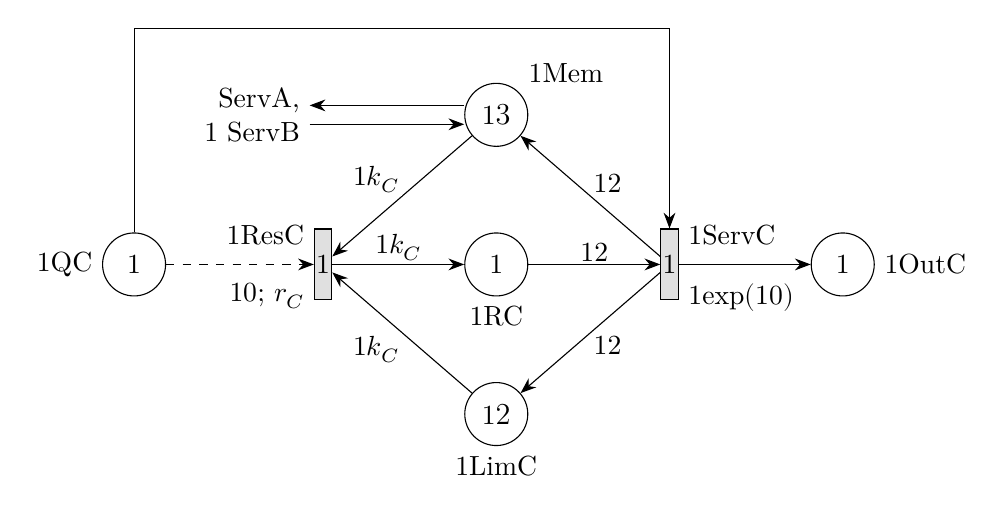
\begin{tikzpicture}[
    font=\setstretch{1}\fontsize{11}{13}\selectfont, >={Stealth[length=2mm]},
    pl/.style={draw, circle, minimum size=8mm, inner sep=0pt},
    tr/.style={draw, fill=black!12, rectangle, minimum width=2.2mm, minimum height=9mm, inner sep=0pt},
    arc/.style={->},
    rd/.style={->, dashed},
    nm/.style={font=\setstretch{1}\fontsize{10}{12}\selectfont},
    par/.style={font=\setstretch{1}\fontsize{10}{12}\selectfont, align=center},
    w/.style={font=\setstretch{1}\fontsize{10}{12}\selectfont, fill=white, inner sep=1pt},
  ]
  \node[pl, label={[nm]left:QC}] (QC) at (0,0) {};
  \node[tr, label={[nm]above left:ResC}, label={[par]below left:$0$; $r_C$}] (ResC) at (2.4,0) {};
  \node[pl, label={[nm]below:RC}] (RC) at (4.6,0) {};
  \node[tr, label={[nm]above right:ServC}, label={[par]below right:$\exp(10)$}] (ServC) at (6.8,0) {};
  \node[pl, label={[nm]right:OutC}] (OutC) at (9.0,0) {};
  \node[pl, label={[nm]above right:Mem}] (Mem) at (4.6,1.9) {3};
  \node[pl, label={[nm]below:LimC}] (LimC) at (4.6,-1.9) {2};
  \node[nm, align=right] (AB) at (1.5,1.9) {ServA,\\ ServB};
  % Дуги
  \draw[rd] (QC) -- (ResC);
  \draw[arc] (QC.north) |- (2.4,3.0) -| (ServC.north);
  \draw[arc] (Mem) -- node[w, above left] {$k_C$} (ResC);
  \draw[arc] (LimC) -- node[w, below left] {$k_C$} (ResC);
  \draw[arc] (ResC) -- node[w, above] {$k_C$} (RC);
  \draw[arc] (RC) -- node[w, above] {2} (ServC);
  \draw[arc] (ServC) -- node[w, above right] {2} (Mem);
  \draw[arc] (ServC) -- node[w, below right] {2} (LimC);
  \draw[arc] (ServC) -- (OutC);
  \draw[arc] ([yshift=1.2mm]Mem.west) -- ([yshift=1.2mm]AB.east);
  \draw[arc] ([yshift=-1.2mm]AB.east) -- ([yshift=-1.2mm]Mem.west);
\end{tikzpicture}

  \caption{Фрагмент мережі Петрі системи з памʼяттю $M = 3$ (решта мережі -- як на
    рисунку~\ref{fig:petri})}
  \label{fig:limc}
\end{figure}

Порівняно з початковою версією \texttt{B14Net} (підрозділ~\ref{sec:structure}) додано позицію
LimC (лише за $M > v_C$, тож за $M = 2$ результати розділу~4 ті самі) і її дуги до ResC та від
ServC; інваріанти~\eqref{eq:mem-invariant} і $m_{\text{LimC}} + m_{\text{RC}} + k_C\,n_{\text{ResC}} +
2\,n_{\text{ServC}} = 2$ у тестових прогонах не порушено:
\codeinput[firstline=61, lastline=61, gobble=8]{../sim/src/main/java/ua/kpi/km/b14/model/B14Net.java}
\medskip
\codeinput[firstline=66, lastline=68, gobble=8]{../sim/src/main/java/ua/kpi/km/b14/model/B14Net.java}
\medskip
\codeinput[firstline=81, lastline=83, gobble=8]{../sim/src/main/java/ua/kpi/km/b14/model/B14Net.java}

Пробний запуск виконано за умов розділу~4 для $s = 1\ldots5$ і $\gamma = 0{,}4\ldots1{,}0$
(за $\rho \le 0{,}78 < 0{,}82$ їх достатньо: критерій~\eqref{eq:criterion} дає $1{,}43\cdot10^6$~хв,
точність -- до 0,98~\%). За потоку з умови задачі система з $M = 3$ стійка за будь-якої стратегії
(рисунок~\ref{fig:imp-w}, таблиця~\ref{tab:imp-base}), а за $\gamma = 0{,}7$ усі відгуки
зменшуються на 70--94~\%, різниця стратегій -- з 2,3~раза до 6,5~\% (таблиця~\ref{tab:imp-compare}).

\begin{figure}
  \centering
  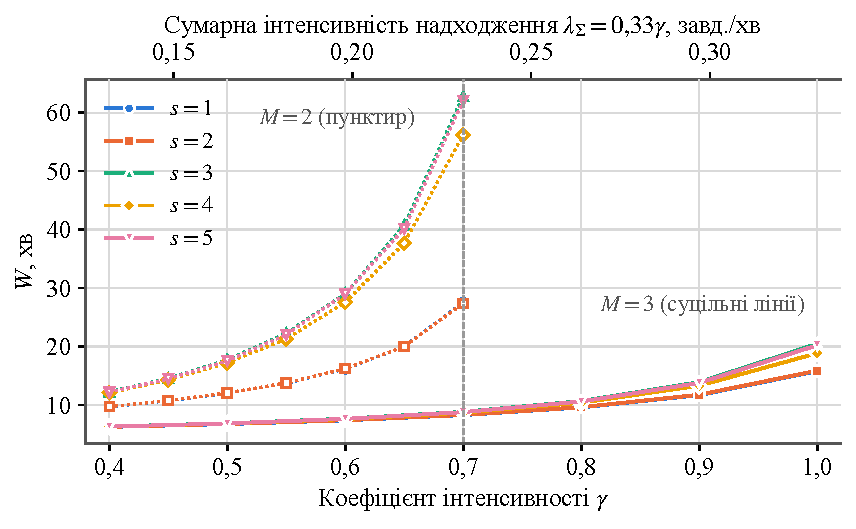
\includegraphics[width=0.7\textwidth]{media/imp-w}
  \caption{Середній час перебування в системі з памʼяттю $M = 2$ і $M = 3$
    ($T_{\text{мод}} = 3{,}5\cdot10^6$~хв, $T_{\text{п}} = 2\cdot10^4$~хв, 60~прогонів; штрихова
    вертикаль -- межа діапазону за $M = 2$)}
  \label{fig:imp-w}
\end{figure}

% Згенеровано experiments/analysis.py — не редагувати вручну
\begin{kpitable}{|c|r|r|r|r|r|r|r|}{Відгуки системи з памʼяттю $M = 3$ за інтенсивностей з умови задачі ($\gamma = 1$, 60 прогонів, $T_{\text{мод}} = 3{,}5\cdot10^6$~хв, $T_{\text{п}} = 2\cdot10^4$~хв)\label{tab:imp-base}}
  {\textbf{$s$} & \textbf{$W$, хв} & \textbf{$L_q$, завд.} & \textbf{$W_q$, хв} & \textbf{$W_A$, хв} & \textbf{$W_B$, хв} & \textbf{$W_C$, хв} & \textbf{$U$}}
  1 & 15,80 $\pm$ 0,04 & 3,46 $\pm$ 0,01 & 10,50 $\pm$ 0,04 & 6,4 & 9,3 & 54,9 & 0,783 \\ \hline
  2 & 15,89 $\pm$ 0,05 & 3,49 $\pm$ 0,02 & 10,58 $\pm$ 0,05 & 7,4 & 6,8 & 54,8 & 0,783 \\ \hline
  3 & 20,46 $\pm$ 0,06 & 5,00 $\pm$ 0,02 & 15,16 $\pm$ 0,06 & 22,9 & 8,3 & 26,5 & 0,784 \\ \hline
  4 & 18,87 $\pm$ 0,06 & 4,48 $\pm$ 0,02 & 13,57 $\pm$ 0,06 & 10,2 & 37,0 & 26,5 & 0,783 \\ \hline
  5 & 20,23 $\pm$ 0,06 & 4,93 $\pm$ 0,02 & 14,92 $\pm$ 0,06 & 21,2 & 12,2 & 26,5 & 0,783 \\ \hline
\end{kpitable}


% Згенеровано experiments/analysis.py — не редагувати вручну
\begin{kpitable}{|c|r|r|r|r|r|r|r|r|r|}{Порівняння відгуків за обсягу памʼяті $M = 2$ і $M = 3$ ($\gamma = 0{,}7$, 60 прогонів, $T_{\text{мод}} = 3{,}5\cdot10^6$~хв, $T_{\text{п}} = 2\cdot10^4$~хв)\label{tab:imp-compare}}
  { & \multicolumn{3}{c|}{\textbf{$W$, хв}} & \multicolumn{3}{c|}{\textbf{$L_q$, завд.}} & \multicolumn{3}{c|}{\textbf{$W_q$, хв}} \\ \cline{2-10}
  \textbf{$s$} & \textbf{$M = 2$} & \textbf{$M = 3$} & \textbf{$\Delta$, \%} & \textbf{$M = 2$} & \textbf{$M = 3$} & \textbf{$\Delta$, \%} & \textbf{$M = 2$} & \textbf{$M = 3$} & \textbf{$\Delta$, \%}}
  1 & 27,53 & 8,29 & $-$70 & 5,14 & 0,69 & $-$87 & 22,23 & 2,99 & $-$87 \\ \hline
  2 & 27,40 & 8,31 & $-$70 & 5,11 & 0,69 & $-$86 & 22,10 & 3,01 & $-$86 \\ \hline
  3 & 62,82 & 8,83 & $-$86 & 13,29 & 0,81 & $-$94 & 57,52 & 3,53 & $-$94 \\ \hline
  4 & 56,20 & 8,70 & $-$85 & 11,75 & 0,78 & $-$93 & 50,90 & 3,40 & $-$93 \\ \hline
  5 & 62,04 & 8,79 & $-$86 & 13,10 & 0,81 & $-$94 & 56,73 & 3,49 & $-$94 \\ \hline
\end{kpitable}


Погіршення відгуків порівняно з $M = 2$ не виявлено (за $\gamma \le 0{,}7$ коротше перебувають
завдання всіх типів). Ціна зміни -- памʼять більша на 50~\% (за $\gamma = 0{,}7$ використання
падає з 0,82 до 0,55) і відмова від монопольного виконання~C; за потоку з умови задачі найдовше
знову чекає тип із найнижчим пріоритетом -- завдання~C у стратегіях 1--2 ($W_{q,C} = 45$~хв
проти 16,5~хв у 3--5) і завдання~B у стратегії~4 ($W_{q,B} = 32$~хв). Висновки щодо вибору
стратегії зберігаються й для системи з $M = 3$: за потоку з умови задачі стратегії 1--2 дають
середній час перебування на 16--23~\% менший, ніж стратегії 3--5 (таблиця~\ref{tab:imp-base}). Дешевша альтернатива -- стратегія 1 або~2 без зміни ресурсу -- за $\gamma = 0{,}7$ скорочує час
перебування у 2,0--2,3~раза, але не дає стійкості за потоку з умови; памʼять -- ще в 3,3~раза. Отже, за потоку, близького до заданого ($\gamma > 0{,}75$), збільшення памʼяті доцільне: лише
воно з розглянутих змін забезпечує роботу системи, а зі стратегією 1 або~2 дає найменший
середній час перебування (15,8~хв). За меншого потоку достатньо вибрати стратегію 1 або~2.

\subsection{Висновки до розділу}

Упорядкування перерозподіляє очікування: стратегії 1 і~2 найкращі загалом, якщо потік не
перевищує трьох чвертей заданого, стратегія~4 -- для завдань~C. Памʼять у три одиниці робить
систему стійкою за потоку з умови задачі й доцільна для нього.

\structural{ВИСНОВКИ}

У курсовій роботі розроблено імітаційну модель інформаційної системи, яка обробляє завдання
трьох типів, що конкурують за оперативну памʼять, з пʼятьма стратегіями пріоритетного
упорядкування черги. Систему формалізовано стохастичною мережею Петрі з 11~позицій і
7~переходів: обмеження на одночасне виконання завдань відтворено позицією памʼяті й кратністю
дуг, стратегії -- пріоритетами та ймовірностями запуску переходів, правило резервування памʼяті
для завдань вищого пріоритету -- переходом резервування з інформаційною дугою. Алгоритм імітації
реалізовано мовою Java на основі ядра PetriObjModelPaint, класи якого використано без змін, а
потрібні модифікації (відтворюваність прогонів, збір статистики після перехідного періоду,
лічильники подій) внесено в класах-нащадках.

Модель відтворює умову задачі з такими припущеннями: надходження завдань -- пуассонівські
потоки; одночасно виконуються не більше двох завдань A і~B; обслуговування без переривання; пріоритет діє на всю чергу, тож завдання нижчого
пріоритету не обходить завдання вищого пріоритету, що чекає памʼяті; за рівних пріоритетів A і~B
вибір між ними випадковий; памʼять -- єдиний обмежений ресурс, а затримки диспетчеризації
нехтовно малі. Інтенсивності надходження з умови задачі не вдалося дослідити в сталому режимі:
система за них перевантажена ($\rho = 1{,}175$), тому мету моделювання досягнуто в області
стійкості -- за спільного зменшення інтенсивностей коефіцієнтом $\gamma \in [0{,}4;\,0{,}7]$, а
нестійкість за $\gamma = 1$ показано окремо; за $\gamma = 0{,}8$ першими втрачають стійкість
стратегії з найнижчим пріоритетом завдань~C.

Верифікація підтвердила коректність моделі: за $4{,}8\cdot10^8$ подій не порушено ні
інваріант памʼяті, ні правила упорядкування; відгуки змінюються в очікуваному напрямі за зміни
кожної вхідної змінної, а для систем M/M/1 і M/M/2 збігаються з аналітичними (до 2~\%). Експериментальне дослідження (перехідний період
$2\cdot10^4$~хв, час моделювання $3{,}5\cdot10^6$~хв, 60~прогонів у точці, точність 2~\% з
довірчою ймовірністю 0,95, 2100~прогонів факторного плану) показало значущий вплив стратегії на
всі три відгуки за кожної інтенсивності. Стратегії A~$>$~B~$>$~C і B~$>$~A~$>$~C
рівноцінні між собою й найкращі за всіма відгуками: середній час перебування в них у
1,25~раза менший за $\gamma = 0{,}4$ і у 2,0--2,3~раза менший за $\gamma = 0{,}7$, ніж у
стратегіях з пріоритетом~C. Ціна цього -- довге перебування завдань~C (за $\gamma = 0{,}7$ до 101~хв проти 22~хв).
Серед стратегій з пріоритетом~C найкраща C~$>$~A~$>$~B. Залежність відгуків від інтенсивності
описано адекватними за критерієм Фішера рівняннями регресії від нормалізованого фактора
$1/(1-\rho)$ з відносною похибкою не більше 1,2~\%.

Запропоновано збільшити памʼять системи з двох до трьох умовних одиниць -- зміну ресурсу, що
знімає монополізацію завдань~C як наслідок. Пробний запуск
показав, що за потоку з умови задачі система стійка із середнім часом
перебування 15,8--20,5~хв, а за $\gamma = 0{,}7$ час перебування скорочується на 70--86~\%,
черга й очікування -- на 86--94~\%; вибір стратегії стійкості не дає, тож за
потоку, близького до заданого, пропозиція доцільна. Отже, мету моделювання
досягнуто: отримано кількісні рекомендації щодо вибору стратегії та ресурсу.

Імітаційний метод дав змогу дослідити систему, для якої через монополізацію ресурсу й
резервування памʼяті аналітичний розвʼязок отримати складно, і кількісно оцінити пропозицію до
її впровадження. Формалізм стохастичної мережі Петрі виявився зручним для цієї задачі: усі
правила системи задано стандартними елементами мережі (кратністю дуг, пріоритетами,
ймовірностями запуску, інформаційною дугою) без спеціальних алгоритмів, а універсальний алгоритм
імітації мережі не залежить від конкретної системи. Найскладнішим було відтворити правило
резервування, бо пріоритети переходів діють лише на одночасно готові події.
Переваги програми -- відтворюваність кожного прогону за seed і висока швидкість: прогін
тривалістю $3{,}5\cdot10^6$~хв виконується менш ніж за секунду.

Подальше дослідження системи доцільно спрямувати на варіювання інтенсивності окремих типів
завдань у ширшому діапазоні, на гібридні стратегії, у яких пріоритет завдання~C зростає з
довжиною його черги, і на вибір обсягу памʼяті за критерієм вартості.

% ДСТУ 8302:2015, за порядком першої згадки. До трьох авторів -- опис із заголовка (перший автор),
% чотири й більше -- з назви, «/ … et al.». Електронні ресурси -- URL і «(дата звернення: …)». Без джерел мовою держави-агресора.
% Склад (вимоги лектора): 1–3 підручники з моделювання, ~1 зі статистики, 1 з ПЗ імітаційного
% моделювання, 1 документація мови програмування (+ документація засобів розробки: Maven, JUnit).
\begin{thebibliography}{99}
\bibitem{stetsenko-kursova} Стеценко І.~В. Моделювання систем. Курсова робота : рек. до виконання курсов. роботи :
  навч. посіб. для здобувачів ступеня бакалавра за освіт. програмою «Інженерія програмного забезпечення
  інформаційних систем» спец. 121 Інженерія програмного забезпечення / І.~В.~Стеценко, О.~Ю.~Дифучина,
  А.~Ю.~Дифучин ; КПІ ім. Ігоря Сікорського. Київ~: КПІ ім. Ігоря Сікорського, 2024. 109~с.
  URL: https://ela.kpi.ua/items/907b5d1f-ca48-4165-a67e-e790ac6fbec5 (дата звернення: 15.11.2026).
\bibitem{stetsenko-modeling} Стеценко І.~В. Моделювання систем : навч. посіб. Черкаси~: ЧДТУ, 2010. 399~с.
\bibitem{java-jls} The Java Language Specification. Java SE 23 Edition / J.~Gosling et al. Oracle, 2024.
  URL: https://docs.oracle.com/javase/specs/jls/se23/html/index.html (дата звернення: 17.11.2026).
\bibitem{petriobjmodelpaint} Стеценко І.~В. PetriObjModelPaint : графічний редактор і симулятор мереж Петрі
  та Петрі-обʼєктних моделей : вихідний код програми. GitHub, 2026.
  URL: https://github.com/StetsenkoInna/PetriObjModelPaint (дата звернення: 16.11.2026).
\bibitem{maven} Apache Maven Project : documentation. The Apache Software Foundation.
  URL: https://maven.apache.org/guides/index.html (дата звернення: 17.11.2026).
\bibitem{junit} JUnit 5 User Guide. Version 5.11.4 / S.~Bechtold et al. JUnit Team, 2024.
  URL: https://junit.org/junit5/docs/5.11.4/user-guide/ (дата звернення: 17.11.2026).
\bibitem{kleinrock} Kleinrock L. Queueing Systems. Vol.~1 : Theory. New York~: Wiley, 1975. 417~p.
\bibitem{scipy} SciPy 1.0 : fundamental algorithms for scientific computing in Python / P.~Virtanen et al.
  \textit{Nature Methods}. 2020. Vol.~17, No.~3. P.~261--272. DOI: 10.1038/s41592-019-0686-2.
\bibitem{java-api} Java Platform, Standard Edition 23 : API Specification. Oracle, 2024.
  URL: https://docs.oracle.com/en/java/javase/23/docs/api/ (дата звернення: 17.11.2026).
\end{thebibliography}


% Лістинги додатків -- 8 пт і типові відступи класу
\fvset{fontsize=\setstretch{1}\fontsize{8}{9}\selectfont, listparameters={}}
\appendices
\appendix{Лістинг алгоритму імітації}
Програма (Java~23) підключає незмінене ядро \texttt{petri-math} 2.6.0
(PetriObjModelPaint~\cite{petriobjmodelpaint}) як залежність. Пакет \texttt{ua.kpi.km.b14.petri} --
розширення ядра, пакет \texttt{ua.kpi.km.b14.model} -- модель системи B14. Допоміжні класи (інтерфейс спостерігача \texttt{SimulationListener}, параметри прогону \texttt{RunSettings}, записи результатів
\texttt{TypeMetrics} і \texttt{SimulationResult}, запис файлів, запуск із командного рядка) не
наведено; повний код програми і скрипта аналізу (каталоги \texttt{sim/} і \texttt{experiments/})
розміщено в репозиторії GitHub \repourl.
\javafile{petri/Delay.java}
\javafile{petri/StochasticTransition.java}
\javafile{petri/ConflictResolver.java}
\javafile{petri/PetriSimulator.java}
\javafile{petri/PetriNetBuilder.java}
\javafile{model/TaskType.java}
\javafile{model/Strategy.java}
\javafile{model/ModelParameters.java}
\javafile{model/B14Net.java}
\javafile{model/OutputCalculator.java}
\javafile{model/B14Simulation.java}

\appendix{Фрагмент протоколу подій}
Протокол сформовано командою \texttt{verify} ($\gamma = 0{,}6$, seed 20261118, файли
\texttt{experiments/verification/protocol\_s3.txt} і \texttt{protocol\_s1.txt}). Стовпці: момент
часу; переходи, з яких вийшли маркери; переходи, у які увійшли маркери (у порядку запуску); стан
після події -- кількість маркерів у позиціях QA, QB, QC, Mem, RC і кількість активних каналів
переходів ServA, ServB, ServC.

\medskip\noindent\textbf{Стратегія 3 (C $>$ B $>$ A), $t \in [0;\,96]$~хв}
\codeinput[firstline=1, lastline=50]{../experiments/verification/protocol_s3.txt}

\medskip\noindent\textbf{Стратегія 1 (A $>$ B $>$ C), $t \in [0;\,38]$~хв}
\codeinput[firstline=1, lastline=23]{../experiments/verification/protocol_s1.txt}

\appendix{Лістинг програми верифікації та експериментального дослідження}
Пакети \texttt{verification} і \texttt{experiment}, статистична частина скрипта
\texttt{experiments/analysis.py}, повні результати верифікації (підрозділ~\ref{sec:verification}),
коефіцієнти регресії й відгуки за типами завдань. Класи \texttt{EventProtocol},
\texttt{ConfidenceInterval}, пакети \texttt{io} і \texttt{app} не наведено (повний код і
результати прогонів -- у репозиторії \repourl).

\begin{kpitable}{|c|c|r|r|r|r|r|r|r|r|r|}{Відгуки моделі за зміни стратегії та коефіцієнта інтенсивності ($T_{\text{мод}} = 3{,}5\cdot10^6$~хв, $T_{\text{п}} = 2\cdot10^4$~хв, 10 прогонів)\label{tab:verif-variation-full}}
  {\textbf{$s$} & \textbf{$\gamma$} & \textbf{$L_q$,} & \textbf{$W_q$,} & \textbf{$W$,} &
   \textbf{$W_{q,A}$,} & \textbf{$W_{q,B}$,} & \textbf{$W_{q,C}$,} & \textbf{$U$} & \textbf{$\rho$} &
   \textbf{$\bar m_{\text{RC}}/M$} \\
   & & \textbf{завд.} & \textbf{хв} & \textbf{хв} & \textbf{хв} & \textbf{хв} & \textbf{хв} & & & }
  1 & 0,4 & 0,58 & 4,40 & 9,70 & 2,88 & 3,55 & 10,47 & 0,470 & 0,470 & 0,000 \\ \hline
  1 & 0,5 & 1,10 & 6,68 & 11,97 & 3,81 & 5,04 & 18,16 & 0,586 & 0,588 & 0,000 \\ \hline
  1 & 0,6 & 2,15 & 10,85 & 16,15 & 4,89 & 7,10 & 35,12 & 0,705 & 0,705 & 0,000 \\ \hline
  1 & 0,7 & 5,21 & 22,55 & 27,86 & 6,10 & 9,69 & 92,34 & 0,823 & 0,823 & 0,000 \\ \hline
  2 & 0,4 & 0,58 & 4,42 & 9,71 & 3,23 & 2,68 & 10,40 & 0,469 & 0,470 & 0,000 \\ \hline
  2 & 0,5 & 1,12 & 6,77 & 12,07 & 4,50 & 3,47 & 18,19 & 0,588 & 0,588 & 0,000 \\ \hline
  2 & 0,6 & 2,16 & 10,91 & 16,22 & 6,06 & 4,28 & 34,83 & 0,705 & 0,705 & 0,000 \\ \hline
  2 & 0,7 & 5,05 & 21,86 & 27,16 & 8,01 & 5,13 & 87,57 & 0,822 & 0,823 & 0,000 \\ \hline
  3 & 0,4 & 0,92 & 6,94 & 12,24 & 7,84 & 5,65 & 5,44 & 0,471 & 0,470 & 0,016 \\ \hline
  3 & 0,5 & 2,03 & 12,32 & 17,62 & 15,03 & 8,91 & 7,25 & 0,587 & 0,588 & 0,022 \\ \hline
  3 & 0,6 & 4,76 & 24,02 & 29,32 & 31,90 & 13,92 & 9,47 & 0,705 & 0,705 & 0,029 \\ \hline
  3 & 0,7 & 13,24 & 57,27 & 62,58 & 83,29 & 21,69 & 12,03 & 0,824 & 0,823 & 0,035 \\ \hline
  4 & 0,4 & 0,91 & 6,88 & 12,18 & 6,50 & 9,12 & 5,50 & 0,471 & 0,470 & 0,016 \\ \hline
  4 & 0,5 & 1,96 & 11,90 & 17,20 & 10,92 & 18,66 & 7,28 & 0,588 & 0,588 & 0,023 \\ \hline
  4 & 0,6 & 4,42 & 22,34 & 27,64 & 18,84 & 43,36 & 9,47 & 0,705 & 0,705 & 0,029 \\ \hline
  4 & 0,7 & 11,68 & 50,54 & 55,84 & 33,99 & 130,93 & 12,01 & 0,822 & 0,823 & 0,035 \\ \hline
  5 & 0,4 & 0,92 & 6,94 & 12,24 & 7,49 & 6,62 & 5,46 & 0,471 & 0,470 & 0,016 \\ \hline
  5 & 0,5 & 2,04 & 12,34 & 17,64 & 14,25 & 11,17 & 7,31 & 0,588 & 0,588 & 0,023 \\ \hline
  5 & 0,6 & 4,66 & 23,53 & 28,83 & 29,46 & 18,65 & 9,45 & 0,704 & 0,705 & 0,029 \\ \hline
  5 & 0,7 & 13,28 & 57,45 & 62,75 & 79,90 & 32,21 & 12,07 & 0,823 & 0,823 & 0,035 \\ \hline
\end{kpitable}

\javafile{verification/InvariantMonitor.java}
\javafile{verification/MmcQueue.java}
\javafile{verification/VerificationRunner.java}
\javafile{experiment/ResponseTrajectory.java}
\javafile{experiment/ExperimentRunner.java}

\par\medskip\noindent Фрагменти файлу \texttt{experiments/analysis.py} (Python, бібліотека
SciPy~\cite{scipy}):
\pyfrag{Критерій~\eqref{eq:criterion} вибору часу моделювання}{143}{151}
\pyfrag{Кількість прогонів за нерівністю Чебишова і критерій згоди $\chi^2$}{269}{290}
\pyfrag{Критерій Кохрена}{406}{417}
\pyfrag{Дисперсійний аналіз впливу стратегії на кожному рівні $\gamma$}{476}{496}
\pyfrag{Регресійний аналіз: метод найменших квадратів, критерії Стьюдента і Фішера}{540}{596}

% Згенеровано experiments/analysis.py — не редагувати вручну
\begin{kpitable}{|c|c|r|r|r|r|r|r|}{Коефіцієнти рівняння регресії~\eqref{eq:regression} для нормалізованого фактора~$x$ (-- доданок відкинуто), індекс кореляції та найбільша відносна похибка\label{tab:exp-regression}}
  {\textbf{Відгук} & \textbf{$s$} & \textbf{$b_0$} & \textbf{$b_1$} & \textbf{$b_2$} & \textbf{$b_3$} & \textbf{$R$} & \textbf{$\delta_{\max}$, \%}}
  $W$ & 1 & 17,822 & 8,495 & 0,801 & 0,415 & 1,00000 & 0,07 \\ \hline
  $W$ & 2 & 17,844 & 8,372 & 0,722 & 0,465 & 1,00000 & 0,05 \\ \hline
  $W$ & 3 & 34,020 & 25,314 & 3,514 & -- & 1,00000 & 0,31 \\ \hline
  $W$ & 4 & 31,880 & 22,400 & 2,271 & $-$0,349 & 1,00000 & 0,13 \\ \hline
  $W$ & 5 & 33,691 & 24,945 & 3,403 & -- & 0,99999 & 0,40 \\ \hline
  $L_q$ & 1 & 2,578 & 2,231 & 0,279 & 0,047 & 1,00000 & 0,55 \\ \hline
  $L_q$ & 2 & 2,582 & 2,208 & 0,261 & 0,055 & 1,00000 & 0,66 \\ \hline
  $L_q$ & 3 & 5,922 & 6,350 & 1,180 & $-$0,162 & 1,00000 & 0,44 \\ \hline
  $L_q$ & 4 & 5,476 & 5,630 & 0,847 & $-$0,199 & 1,00000 & 0,31 \\ \hline
  $L_q$ & 5 & 5,849 & 6,231 & 1,152 & $-$0,129 & 0,99999 & 1,23 \\ \hline
  $W_q$ & 1 & 12,519 & 8,494 & 0,801 & 0,416 & 1,00000 & 0,11 \\ \hline
  $W_q$ & 2 & 12,541 & 8,371 & 0,723 & 0,468 & 1,00000 & 0,09 \\ \hline
  $W_q$ & 3 & 28,717 & 25,315 & 3,513 & -- & 1,00000 & 0,54 \\ \hline
  $W_q$ & 4 & 26,577 & 22,399 & 2,270 & $-$0,347 & 1,00000 & 0,17 \\ \hline
  $W_q$ & 5 & 28,387 & 24,944 & 3,404 & -- & 0,99999 & 0,71 \\ \hline
\end{kpitable}

% Згенеровано experiments/analysis.py — не редагувати вручну
\begin{kpitable}{|c|c|r|r|r|r|r|r|r|r|}{Відгуки за типами завдань (середнє за 60 прогонами, $T_{\text{мод}} = 3{,}5\cdot10^6$~хв, $T_{\text{п}} = 2\cdot10^4$~хв)\label{tab:exp-bytype}}
  {\textbf{$s$} & \textbf{$\gamma$} & \textbf{$W_A$, хв} & \textbf{$W_B$, хв} & \textbf{$W_C$, хв} & \textbf{$W_{q,A}$, хв} & \textbf{$W_{q,B}$, хв} & \textbf{$W_{q,C}$, хв} & \textbf{$U$} & \textbf{$\bar m_{\text{RC}}/M$}}
  1 & 0,40 & 6,89 & 8,54 & 20,49 & 2,89 & 3,54 & 10,48 & 0,470 & 0,000 \\ \hline
  1 & 0,45 & 7,34 & 9,26 & 23,76 & 3,34 & 4,26 & 13,76 & 0,529 & 0,000 \\ \hline
  1 & 0,50 & 7,82 & 10,07 & 28,30 & 3,82 & 5,07 & 18,30 & 0,587 & 0,000 \\ \hline
  1 & 0,55 & 8,34 & 11,01 & 34,85 & 4,34 & 6,01 & 24,85 & 0,646 & 0,000 \\ \hline
  1 & 0,60 & 8,89 & 12,08 & 45,25 & 4,89 & 7,08 & 35,25 & 0,705 & 0,000 \\ \hline
  1 & 0,65 & 9,47 & 13,29 & 63,04 & 5,46 & 8,29 & 53,04 & 0,764 & 0,000 \\ \hline
  1 & 0,70 & 10,07 & 14,67 & 100,73 & 6,07 & 9,67 & 90,73 & 0,823 & 0,000 \\ \hline
  2 & 0,40 & 7,24 & 7,70 & 20,40 & 3,24 & 2,70 & 10,40 & 0,470 & 0,000 \\ \hline
  2 & 0,45 & 7,84 & 8,07 & 23,66 & 3,84 & 3,07 & 13,67 & 0,529 & 0,000 \\ \hline
  2 & 0,50 & 8,51 & 8,47 & 28,16 & 4,51 & 3,47 & 18,16 & 0,588 & 0,000 \\ \hline
  2 & 0,55 & 9,25 & 8,87 & 34,64 & 5,25 & 3,87 & 24,64 & 0,646 & 0,000 \\ \hline
  2 & 0,60 & 10,07 & 9,28 & 44,81 & 6,07 & 4,28 & 34,81 & 0,705 & 0,000 \\ \hline
  2 & 0,65 & 10,99 & 9,71 & 62,06 & 6,99 & 4,71 & 52,05 & 0,764 & 0,000 \\ \hline
  2 & 0,70 & 12,02 & 10,15 & 98,80 & 8,02 & 5,15 & 88,80 & 0,823 & 0,000 \\ \hline
  3 & 0,40 & 11,85 & 10,68 & 15,46 & 7,85 & 5,68 & 5,45 & 0,470 & 0,016 \\ \hline
  3 & 0,45 & 14,86 & 12,16 & 16,34 & 10,86 & 7,16 & 6,34 & 0,529 & 0,019 \\ \hline
  3 & 0,50 & 19,19 & 14,00 & 17,32 & 15,19 & 9,00 & 7,31 & 0,588 & 0,022 \\ \hline
  3 & 0,55 & 25,56 & 16,20 & 18,34 & 21,56 & 11,20 & 8,34 & 0,646 & 0,026 \\ \hline
  3 & 0,60 & 35,54 & 18,89 & 19,45 & 31,54 & 13,89 & 9,45 & 0,705 & 0,029 \\ \hline
  3 & 0,65 & 53,17 & 22,33 & 20,68 & 49,17 & 17,33 & 10,68 & 0,764 & 0,032 \\ \hline
  3 & 0,70 & 87,76 & 26,62 & 22,01 & 83,76 & 21,62 & 12,01 & 0,823 & 0,035 \\ \hline
  4 & 0,40 & 10,41 & 13,99 & 15,46 & 6,41 & 8,99 & 5,45 & 0,470 & 0,016 \\ \hline
  4 & 0,45 & 12,39 & 17,88 & 16,35 & 8,39 & 12,88 & 6,34 & 0,529 & 0,019 \\ \hline
  4 & 0,50 & 14,92 & 23,65 & 17,31 & 10,92 & 18,65 & 7,31 & 0,587 & 0,023 \\ \hline
  4 & 0,55 & 18,23 & 32,62 & 18,32 & 14,23 & 27,61 & 8,32 & 0,646 & 0,026 \\ \hline
  4 & 0,60 & 22,80 & 48,06 & 19,46 & 18,80 & 43,06 & 9,46 & 0,705 & 0,029 \\ \hline
  4 & 0,65 & 29,15 & 76,57 & 20,69 & 25,15 & 71,57 & 10,69 & 0,764 & 0,032 \\ \hline
  4 & 0,70 & 38,19 & 136,96 & 22,02 & 34,19 & 131,96 & 12,02 & 0,822 & 0,035 \\ \hline
  5 & 0,40 & 11,44 & 11,56 & 15,45 & 7,44 & 6,57 & 5,45 & 0,470 & 0,016 \\ \hline
  5 & 0,45 & 14,23 & 13,58 & 16,34 & 10,23 & 8,58 & 6,35 & 0,529 & 0,019 \\ \hline
  5 & 0,50 & 18,17 & 16,10 & 17,29 & 14,17 & 11,10 & 7,29 & 0,587 & 0,022 \\ \hline
  5 & 0,55 & 24,10 & 19,35 & 18,33 & 20,10 & 14,35 & 8,33 & 0,646 & 0,026 \\ \hline
  5 & 0,60 & 33,69 & 23,76 & 19,49 & 29,69 & 18,75 & 9,48 & 0,705 & 0,029 \\ \hline
  5 & 0,65 & 49,81 & 29,33 & 20,68 & 45,81 & 24,33 & 10,68 & 0,764 & 0,032 \\ \hline
  5 & 0,70 & 82,78 & 37,08 & 22,03 & 78,78 & 32,08 & 12,03 & 0,823 & 0,035 \\ \hline
\end{kpitable}

\end{document}
